\chapter{Search for Supersymmetry and Dark Matter in Events with Dileptons and Missing Energy}
\label{sec:CandCanalysis}

%Beskriv prosessene her istedet for i teori og motiver hvordan partiklene er produsert. 

This chapter will introduce the search for new physics through various processes we explain, how the signal and background samples are produced, and how we perform a traditional so-called cut and count analysis when searching for new particles or phenomena in LHC data. We will show the results obtained by the ATLAS collaboration and compare them to results we otained following a similar strategy as in the publication. 



The processes we are interested in looking at in this thesis involve superpartners of leptons, gauge bosons, and the Higgs boson. Besides this, we will look at a dark matter particle candidate, which is predicted to be the lightest supersymmetric particle (LSP).  This thesis looks at proton-proton collisions with final state two leptons and missing transverse energy (MET/$E_T^{miss}$). The SUSY processes we are looking at are direct slepton production, chargino production with slepton/sneutrino-mediated-decays and with W-boson-mediated-decays. 


In figure \ref{fig:SlepSlepFeynman} below, we can see the direct slepton production as a production of two hypothetical sleptons which decay to the final state, comprising of two leptons and missing transverse energy (i.e. missing energy in the detector). The neutralinos, which are the MET in this process, are a mixture of the sparticles photino, zino, and higgsino and is also one of the dark matter candidates mentioned above.  
\begin{figure}[H]
    \centering
    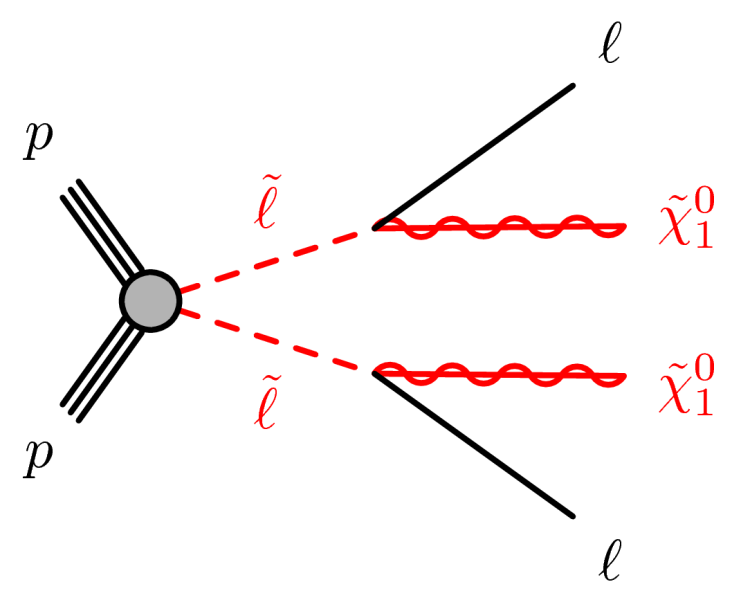
\includegraphics[width = 0.4\textwidth]{Figures/FeynmanDiagrams/SlepSlepFeynman.png}
    \caption{Direct slepton production $pp \rightarrow \tilde{l}^+ \tilde{l}^- \rightarrow l^+l^- + \tilde{\chi}_1^0 \tilde{\chi}_1^0$.}
    \label{fig:SlepSlepFeynman}
\end{figure}

In figure \ref{fig:SlepSnuFeynman} and \ref{fig:WWFeynman} we can see the chargino production with  slepton/sneutrino-mediated-decays and with W-boson-mediated-decays. Charginos are a mixture of the sparticles wino and the charged higgsino. These processes have the same final state as direct slepton production, but here the neutrinos are also a part of the MET, since we can't actually detect them in the detector. 
\begin{figure}[H]
    \centering
    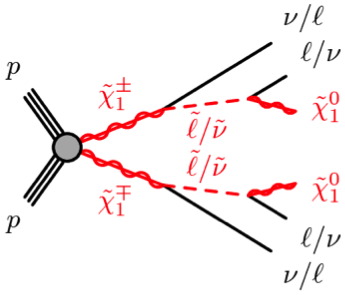
\includegraphics[width = 0.4\textwidth]{Figures/FeynmanDiagrams/SlepSnuFeynman.png}
    \caption{Chargino production with slepton/sneutrino-mediated-decays $pp \rightarrow \tilde{\chi}_1^+ \tilde{\chi}_1^- \rightarrow \tilde{l}^+ \tilde{l}^- /\tilde{\nu} \tilde{\nu} \rightarrow l^+l^- + \nu \Bar{\nu} + \tilde{\chi}_1^0 \tilde{\chi}_1^0$.}
    \label{fig:SlepSnuFeynman}
\end{figure}

\begin{figure}[H]
    \centering
    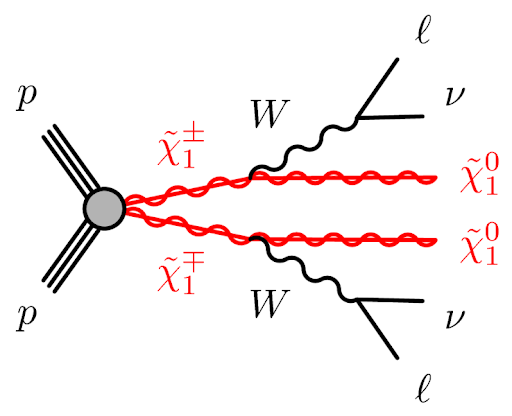
\includegraphics[width = 0.4\textwidth]{Figures/FeynmanDiagrams/WWFeynman.png}
    \caption{Chargino production with W-boson-mediated-decays $pp \rightarrow \tilde{\chi}_1^+ \tilde{\chi}_1^- \rightarrow W^+ W^- \rightarrow l^+l^- + \nu \Bar{\nu} + \tilde{\chi}_1^0 \tilde{\chi}_1^0$.}
    \label{fig:WWFeynman}
\end{figure}

The DM process we are looking at in this thesis is the mono-Z process shown in figure \ref{fig:monoZFeynman2}. Here we have a mediator V which decays into the DM particles $\chi$ and a W/Z that decays into two leptons. This gives us the same final state as we had for the SUSY processes.  

\begin{figure}[H]
    \centering
    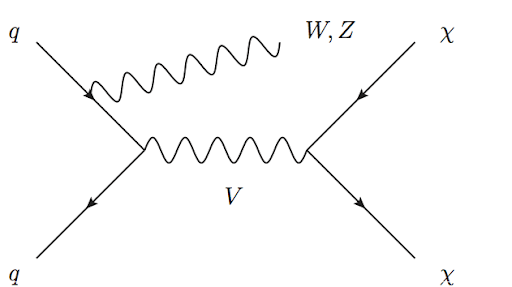
\includegraphics[width = 0.4\textwidth]{Figures/FeynmanDiagrams/monoZFeynman2.png}
    \caption{Mono-Z process $pp \rightarrow Z + MET \rightarrow l^+ l^- + MET$.}
    \label{fig:monoZFeynman2}
\end{figure}


\section{MC simulated events}

The data taken into consideration is from the ATLAS experiment at LHC between 2015-2018 (Run 2), further explained in chapter \ref{sec:LHCandATLAS}. But, we are also looking at some MC simulated background and signal which will be explained in this section. The explanations are taken from the publications from ATLAS, namely \cite{sleptonexclusion} for the SUSY signals and \cite{monoZexclusion} for the mono-Z signal. We present an overview of what signal samples that are used in table \ref{tab:directslepLOW} - \ref{tab:MonoZHigh} in section \ref{sec:sigsamptab}. 

The SUSY signal samples were generated from leading-order (LO) matrix elements with up to two extra partons using \textsc{MadGraph5\_aMC@NLO 2.6.1} \cite{48} interfaced to \textsc{Pythia 8.186} \cite{49}, with the A14 tune \cite{50}, for the modelling of the SUSY decay chain, parton showering, hadronisation and the description of the underlying event. Parton luminosities were provided by the NNPDF2.3LO PDF set \cite{51}. Jet–parton matching was performed following the CKKW-L prescription \cite{52}, with a matching scale set to one quarter of the mass of the pair-produced SUSY particles. Signal cross-sections were calculated to next-to-leading order (NLO) in $\alpha_s$ adding the resummation of soft gluon emission at next-to-leading-logarithm accuracy(NLO+NLL) \cite{53,54,55,56,57,58,59}. The nominal cross-sections and their uncertainties were taken from an envelope of cross-section predictions using different PDF sets and factorisation and renormalisation scales, as described in Ref. \cite{60}. 


To study the invisible Higgs boson decays, Monte Carlo events are produced for the SM ZH process with a subsequent Z boson decay into a dilepton pair and the H$\rightarrow$ZZ$\rightarrow \nu \nu \nu \nu$ decay (ZH$\rightarrow ll$+inv). The ZH signal processes from both the quark–antiquark (qqZH) and gluon–gluon (ggZH) initial states are modelled with \textsc{Powheg-Box v2} \cite{49Z, 50Z} using the CT10 \cite{51Z} parton distribution function (PDF) and interfaced to \textsc{Pythia8.186} \cite{52Z} for parton showering. The kinematic distributions of ZH$\rightarrow ll$ +inv events are described at next-to-leading-order (NLO) in QCD. Additionally, for the qqZH process, the MINLO \cite{53Z} method is applied to improve the gluon resummation calculation, and the $p_T^Z$ distribution is corrected to NLO electroweak (EW) accuracy with a reweighting approach detailed in Ref. \cite{3Z}. The SM ZH production cross-section is computed with next-to-next-to-leading-order (NNLO) QCD and NLO EW precision and found to be 884 fb \cite{3Z} with $m_H = 125$ GeV at 13 TeV. The DM signal is modelled with the leading-order \textsc{MadGraph5\_aMC@NLO} matrix element \cite{54Z} using NNPDF3.0 \cite{55Z} and showered with Pythia8.186. DM signal events with an axial-vector mediator and fermionic WIMPs are produced for different $m_{med}$ and $m_\chi$, both in a range from 10 to 1000 GeV.  As recommended in Ref. \cite{44Z}, the DM events are generated by choosing $g_q = 0.25$, $g_\chi = 1$, and a minimal mediator width. The AZNLO \cite{56Z} and A14 \cite{57Z} parameter sets are used to tune the \textsc{Pythia8.186} parton-shower for the simulation of the ZH $\rightarrow ll$+inv and DM signals, respectively.


The different backgrounds that we are considering are diboson, triboson, $t\Bar{t}$, single top, other top events ($t\Bar{t}$ events with a pair of leptons or boson(s)), Higgs, Drell-Yan, Z+jets and W+jets. The MC samples are simulated using different generators that are listed up in table \ref{tab:bkg_samples}. The goal is to separate these backgrounds from the signals we are looking at, which consist in the four different processes that we looked at earlier in this chapter. 

\begin{table}[H]
    \centering
    \begin{tabular}{l l l l} \toprule
        \textbf{Background sample} & \textbf{Generator} & \textbf{Parton shower} & \textbf{Normalisation}\\
        \midrule
        \midrule
        Diboson & \textsc{Sherpa2.2.2}\cite{sherpa2_1, sherpa1_2, sherpa1_3} & \textsc{Sherpa2.2.2} & NLO \cite{NLO}\\
        Triboson & \textsc{Sherpa2.2.2} & \textsc{Sherpa2.2.2} & NLO \\
        Z+jets & \textsc{Sherpa2.2.1} \cite{sherpa1_1, sherpa1_2, sherpa1_3} & \textsc{Sherpa2.2.1} & NNLO \cite{NNLO}\\
        W+jets & \textsc{Powheg-Box v2}\cite{49Z, 50Z} & \textsc{Pythia8.186} \cite{49} & NLO\\
        Drell-Yan & \textsc{Sherpa2.2.1} & \textsc{Sherpa2.2.1} & NNLO\\
        $t\Bar{t}$ & \textsc{Powheg-Box v2} & \textsc{Pythia8.186} & NNLO\\
        Single top & \textsc{Powheg-Box v2} & \textsc{Pythia8.186} & NLO\\
        topOther & \textsc{MG5\_aMC@NLO} \cite{48} & \textsc{Pythia8.186} & NLO\\
        Higgs & \textsc{Powheg-Box v2} & \textsc{Pyhtia8.186} & NLO\\
        \bottomrule
    \end{tabular}
    \caption{An overview of the different generators used to simulate the MC background samples.}
    \label{tab:bkg_samples}
\end{table}


Before we move on to how we perform the analysis, we also need to know how we are going to know that we see SUSY and DM particles in the detector. Since they never have been discovered, we have to lean on some hypotheses on how this is happening. As for all events in the detector, we have to reconstruct the events using their decays. The supersymmetric particles are expected to decay into cascades that will contain a LSP which will interact very weakly with the detector material which again will result in a big measured MET in the detector. The rest of the cascade will result in a final state with with leptons and/or jets. Together with the MET this gives us the final state we are looking for. For the mono-Z process we can measure the MET from the DM particles decayed from the unknown hypothetical mediator particle. Together with the leptons we get from the decay of the Z-boson, this gives us the same final state as for the SUSY processes.




































\begin{comment}

\begin{itemize}
    \item Bruker noe som eksisterer
    \item Tradisjonell måte ting har blitt gjort på
    \item begrenset av menneskets forståelse av prosessen vi ser på
    \item vi må bestemme alle kuttene som blir gjort
    \item Du må vite hva du skal se etter for å gjøre dette, altså trenger en teori/hypotese
    \item Tenk overgang til ML
    \item Valg må være begrunnet 
    \item Massesplitting. Cut and count er svak på lav massesplitting. Dette gjør ML bedre
\end{itemize}
\end{comment}








\section{The standard way: cut and count}
\label{sec:candc}

The first part of the analysis done in this thesis is a traditional cut and count analysis. \textit{Cut and count} is probably the most known method used in particle physics and has proved to be very useful in the discoveries we have done so far. Since the data become more and more massive and complex, and the processes we are looking at more and more complicated, we also need to develop further and improve the way we perform the analysis. In this thesis, we are mainly going to focus on machine learning algorithms. Therefore we have not tried to improve this standard way to analyze data and have based the cut and count on already published analyses from ATLAS \cite{sleptonexclusion, monoZexclusion}. 

In cut and count, we select events sensitive to new physics, by reducing as much as possible any SM background processes which could mimic the signal. After applying several cuts, the selection of events we are left with form the so-called \textit{signal region}. We then see whether the expected signal is significantly separated from the expected Standard Model (SM) background in this region. We can calculate an expected significance $Z$, which will be explained in section \ref{sec:significance} later in the thesis, to check if we can expect to claim a discovery in this region if a particular signal model turns out to be realized in nature. If we are lucky and have cut away enough background and kept sufficient signal, we can check if the observed events in data are compatible with the signal+background hypothesis or if they match the background-only hypothesis (i.e. no signal) instead. Let us consider the case where the data differ from the background and tends to follow the signal: we know that there is most likely something interesting in this region.

Of course, there are advantages and disadvantages with every method, and this is also the case for cut and count. In cut and count, we need a theory or hypothesis as a reference to know what kind of signals we should look for. We are also only able to do cuts in one or two dimensions and adjust the different variables to our purposes to a certain complexity. It is therefore unfortunately limited by the human understanding of what we are looking at. The lack of human understanding is where Machine Learning (ML) comes to help. The ML methods are expected to help us better separate the signal from the background and can look at the data in several dimensions and with more complexity. This is further explained in the following chapters, where we will look at what the different ML methods do.






\section{Reproducing the ATLAS publications}
The first part of this analysis was done by cut and count and the goal was to reproduce the results from publications done by ATLAS \cite{sleptonexclusion, monoZexclusion}. Here we will compare our results to the official results from the ATLAS experiment, and hopefully achieve a good agreement between the two.

Since the goal is to reproduce the results, we implement more or less the same analysis procedure as described in the publications. The cuts done for the SUSY processes are listed in table \ref{tab:cutsSUSY} and for the mono-Z process in table \ref{tab:cutsDM}, where both tables are taken from the publications \cite{sleptonexclusion, monoZexclusion}. All the kinematic variables we cut on are presented in chapter \ref{sec:LHCandATLAS}, except the tagging of b-jets which are jets initiated by bottom quarks. All of the results are presented with a systematic uncertainty. The first cut we do for both processes is to demand exactly two leptons with opposite signs in the final state.


\begin{table}[H]
    \centering
    \begin{tabular}{l l}\toprule
    \textbf{Variables} & \textbf{Cuts}\\
    \midrule
    \midrule
    Two leptons & Same flavor (SF) and opposite sign (OS)\\
    $n_{\text{jets}}$     & 0 \\
    $m_{ll}$ [GeV]     & 121.2\\
    $E_T^{miss}$ [GeV] & $>$ 110 \\
    $E_T^{miss}$ significance & $>$ 10\\
    $m_{T2}$ [GeV] & 160\\
    \bottomrule
    \end{tabular}
    \caption{Cuts added in the cut and count analysis taken from the publication for the SUSY processes \cite{sleptonexclusion}.}
    \label{tab:cutsSUSY}
\end{table}

For the SUSY processes we have applied the cuts in table \ref{tab:cutsSUSY}, where we, in addition to having only two leptons with opposite sign in the final state, demand that they have to have the same flavor as well. Here we get the Z+jets as the dominating background as we can see in both figure \ref{fig:nJetSUSY} and table \ref{tab:cutflowSUSY}. Now we want to reduce all of the background, especially Z+jets, and we apply the next cut in table \ref{tab:cutsSUSY} which is demanding no jets (both b-tagged and non-b-tagged). As we can see in figure \ref{fig:mllSUSY}, the Z+jets background is still the dominating background, but if we look at table \ref{tab:cutflowSUSY}, we can see that it is reduced a lot. The reason for Z+jets is still dominating is that the jet-cut reduced around the same percentage from all of the different backgrounds. 

\begin{figure}[H]
\centering
    \begin{subfigure}[t!]{0.49\textwidth}
        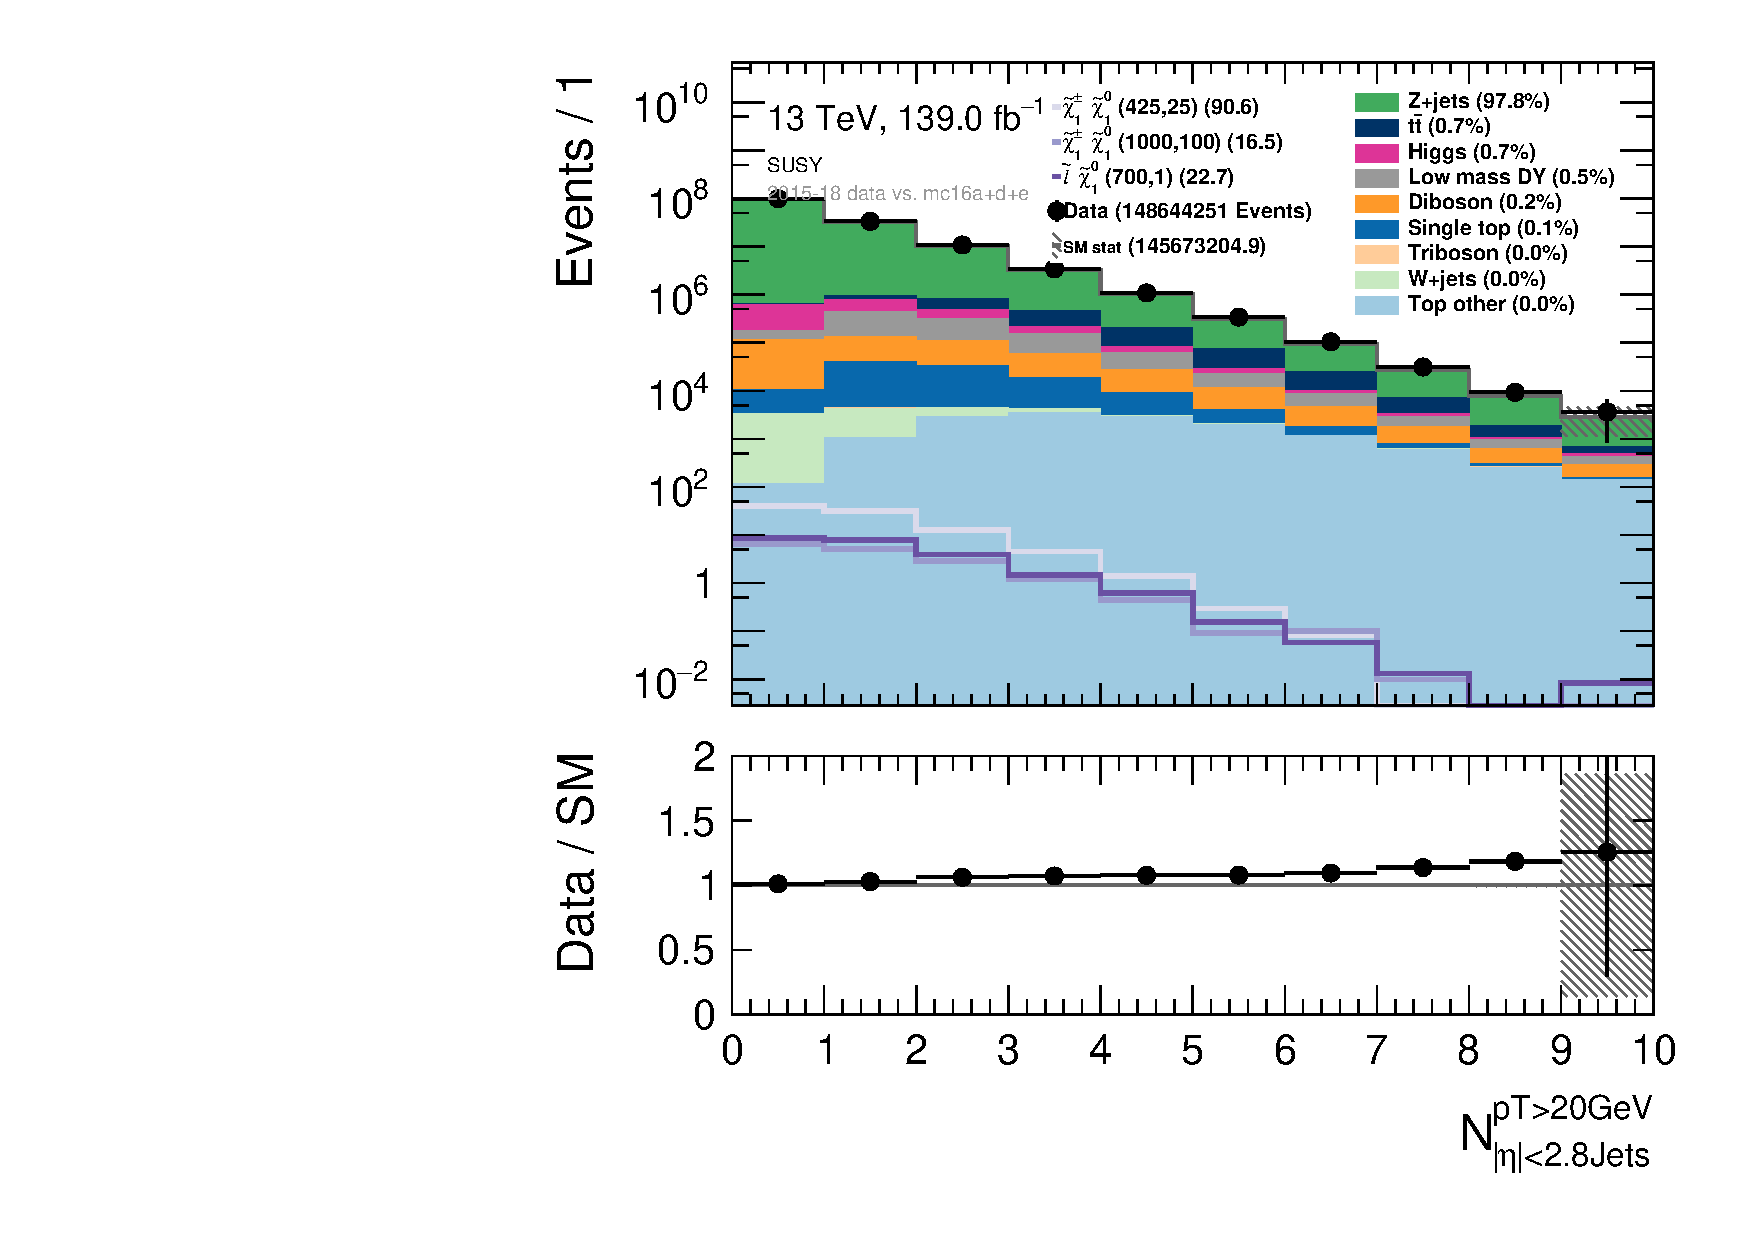
\includegraphics[width=\textwidth]{Figures/SUSYcuts/hist1d_nJet20_SUSY.pdf}
    \caption{Number of jets with a $p_T > 20$ GeV.}
    \label{fig:nJetSUSY}
    \end{subfigure}
    \begin{subfigure}[t!]{0.49\textwidth}
        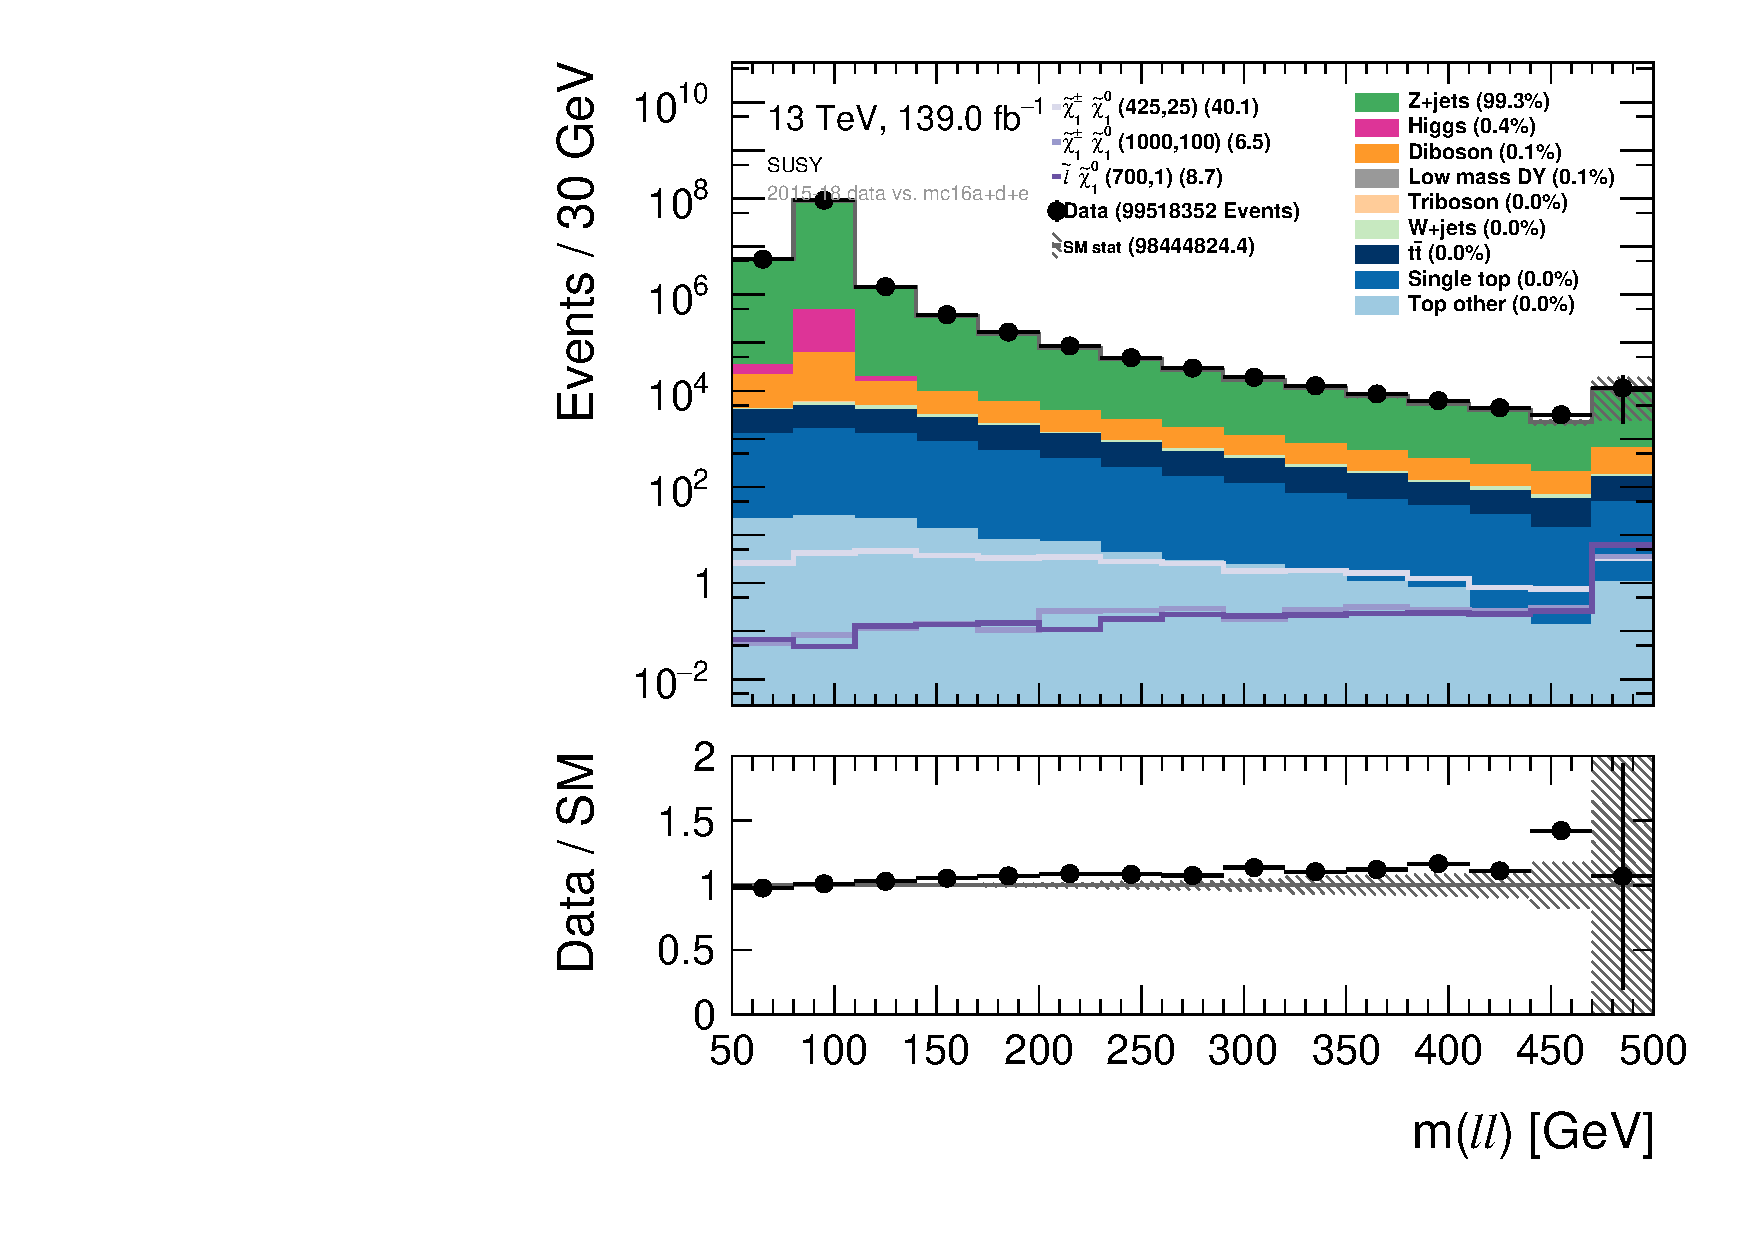
\includegraphics[width=\textwidth]{Figures/SUSYcuts/hist1d_mll_SUSY.pdf}
    \caption{The invariant mass of the two leptons.}
    \label{fig:mllSUSY}
    \end{subfigure}
    \caption{Plot of different distributions after applying the cuts on 2L, SF, OS (a) and no jets (b).}
    \label{fig:stepsSUSY1}
\end{figure}


The next cut we have applied is on the invariant mass of the two leptons in the final state. The results are shown in figure \ref{fig:metSUSY} and as we can see, most of the background is reduced by a lot. We have also done a cut requiring large missing transverse energy. This is done because it cuts away more background than signal, which entails obtaining a more significant separation between the signal and background. By applying this cut, we can see that the Z+jets are no longer the dominating background and the results are shown in figure \ref{fig:metSignSUSY} and table \ref{tab:cutflowSUSY}. 

\begin{figure}[H]
    \centering
    \begin{subfigure}[t!]{0.49\textwidth}
        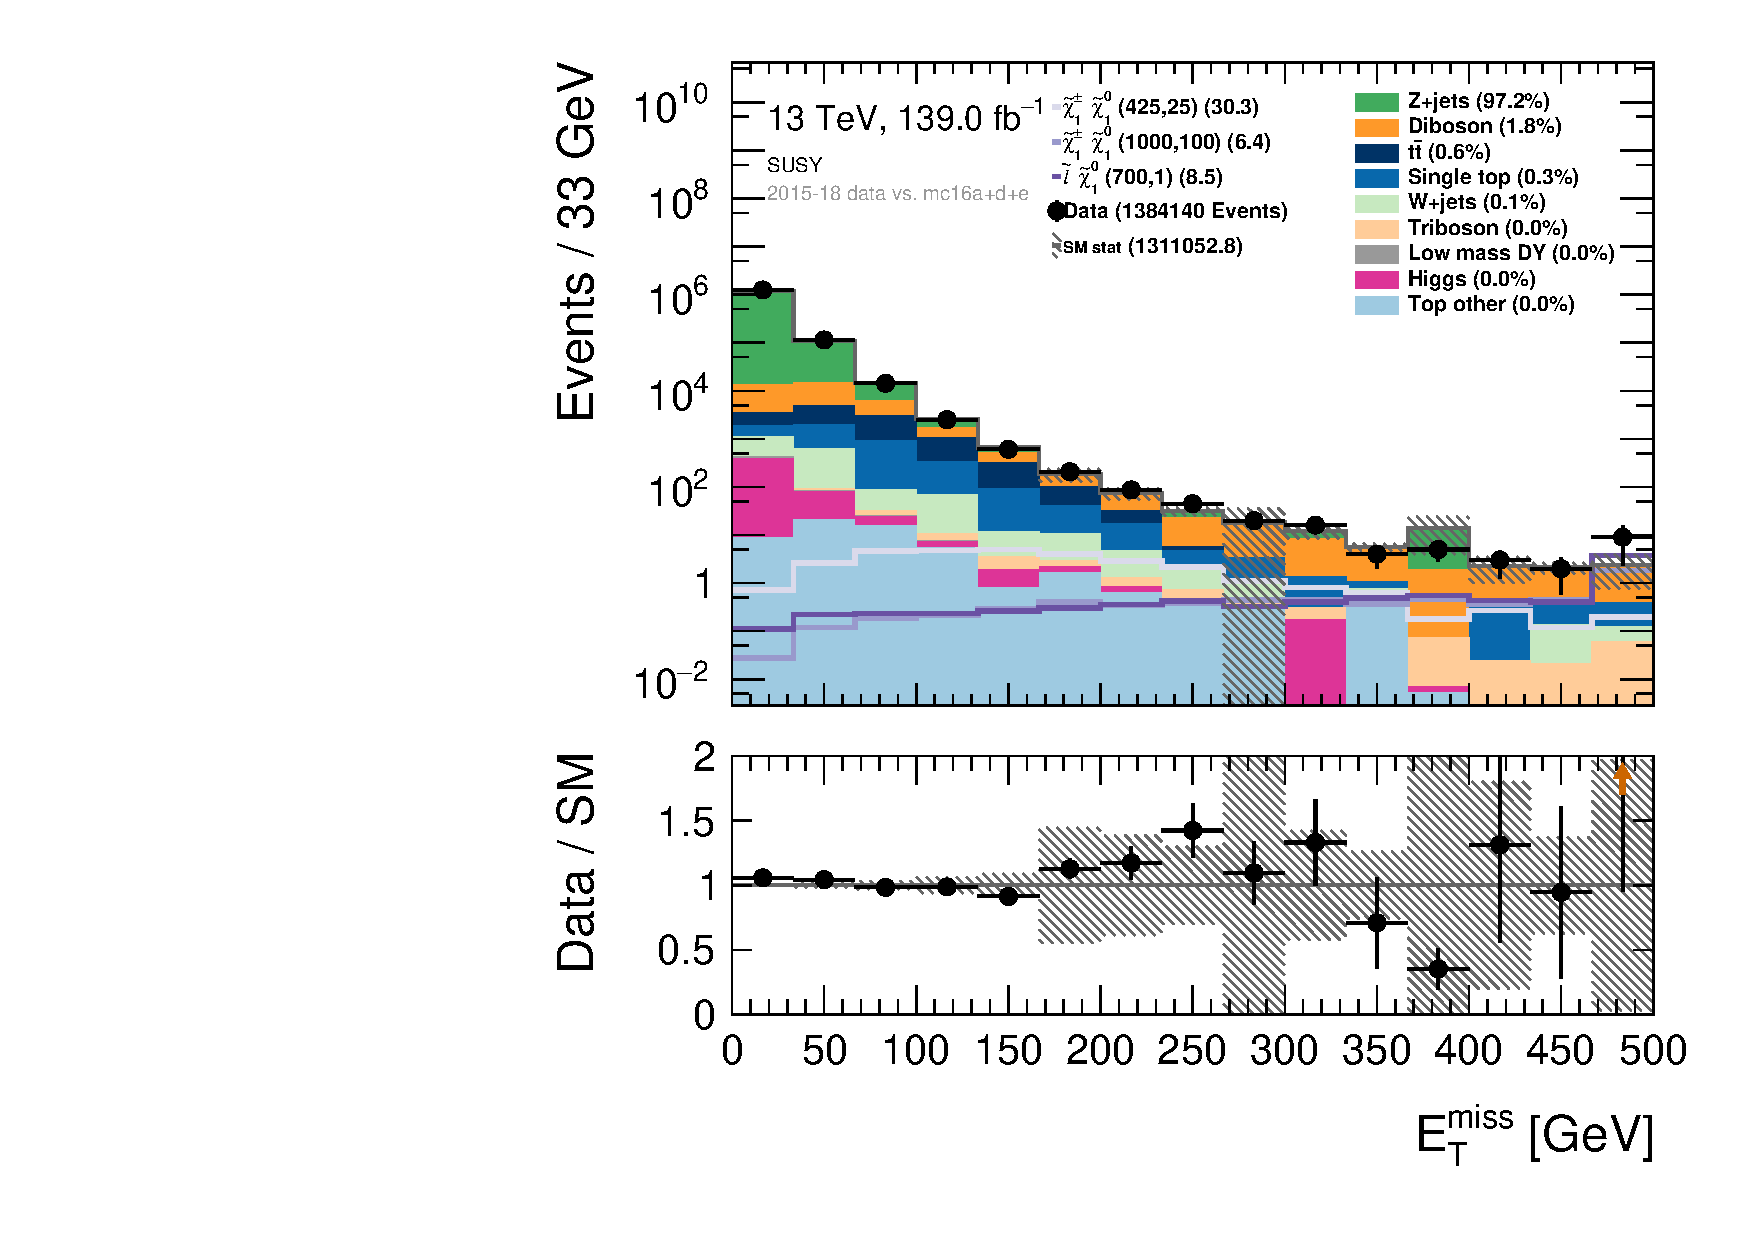
\includegraphics[width=\textwidth]{Figures/SUSYcuts/hist1d_met_Et_SUSY.pdf}
    \caption{Missing transverse energy.}
    \label{fig:metSUSY}
    \end{subfigure}
    \begin{subfigure}[t!]{0.49\textwidth}
        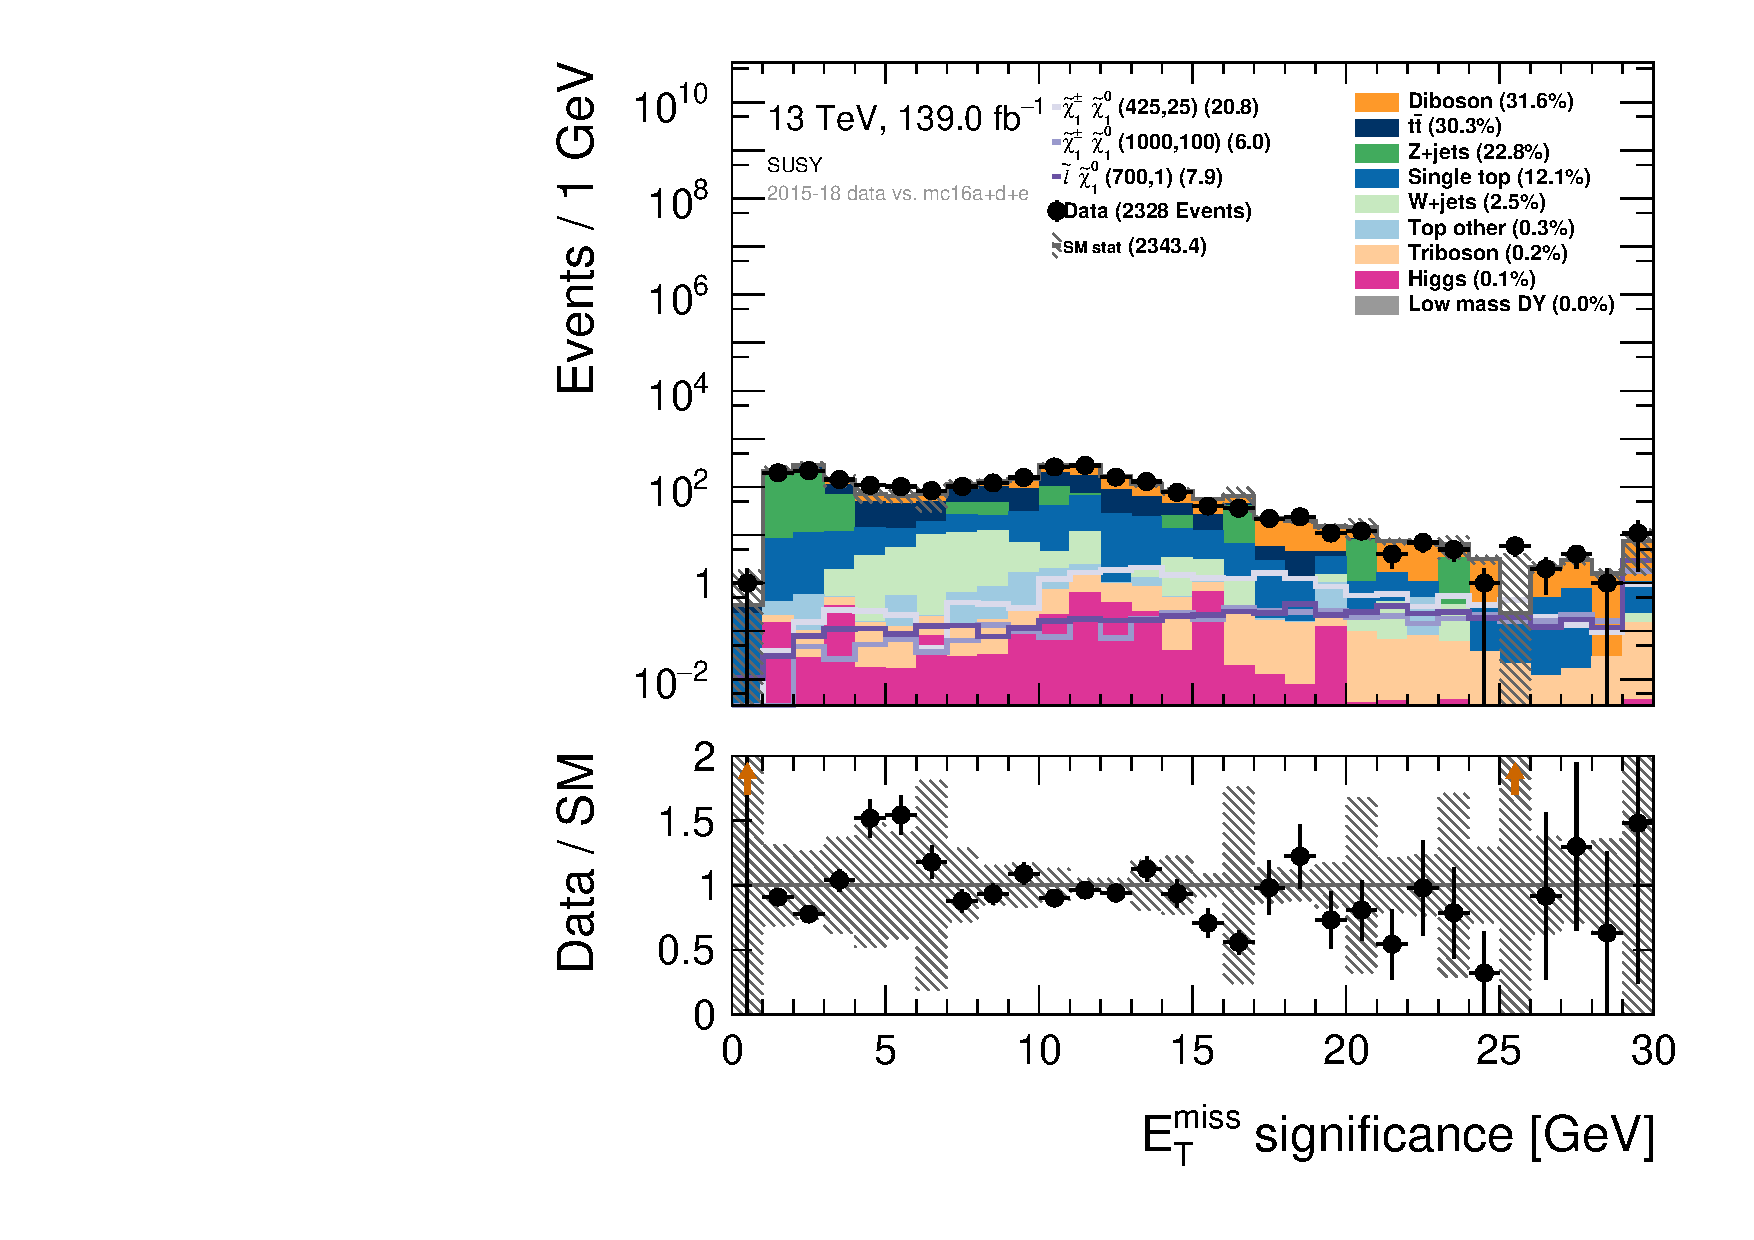
\includegraphics[width=\textwidth]{Figures/SUSYcuts/hist1d_met_Sign_SUSY.pdf}
    \caption{Missing transverse energy significance.}
    \label{fig:metSignSUSY}
    \end{subfigure}
    \caption{Plot of different distributions after applying the cuts on the invariant mass (a) and MET (b).}
    \label{fig:stepsSUSY2}
\end{figure}


The last two cuts applied is a cut on the MET significance and $m_{T2}$. The results after applying the MET significance cut is shown in figure \ref{fig:stepsSUSY3} and as we can see, the diboson is still the dominating background. The last cut that are applied for the SUSY processes are on the $m_{T2}$ variable. This is done to get rid of the rest of the $t\Bar{t}$ background and leave us more or less with only diboson. This is part of our final result and are shown in figure \ref{fig:cutandcountMONA} later in this section.

\begin{figure}[H]
    \centering
        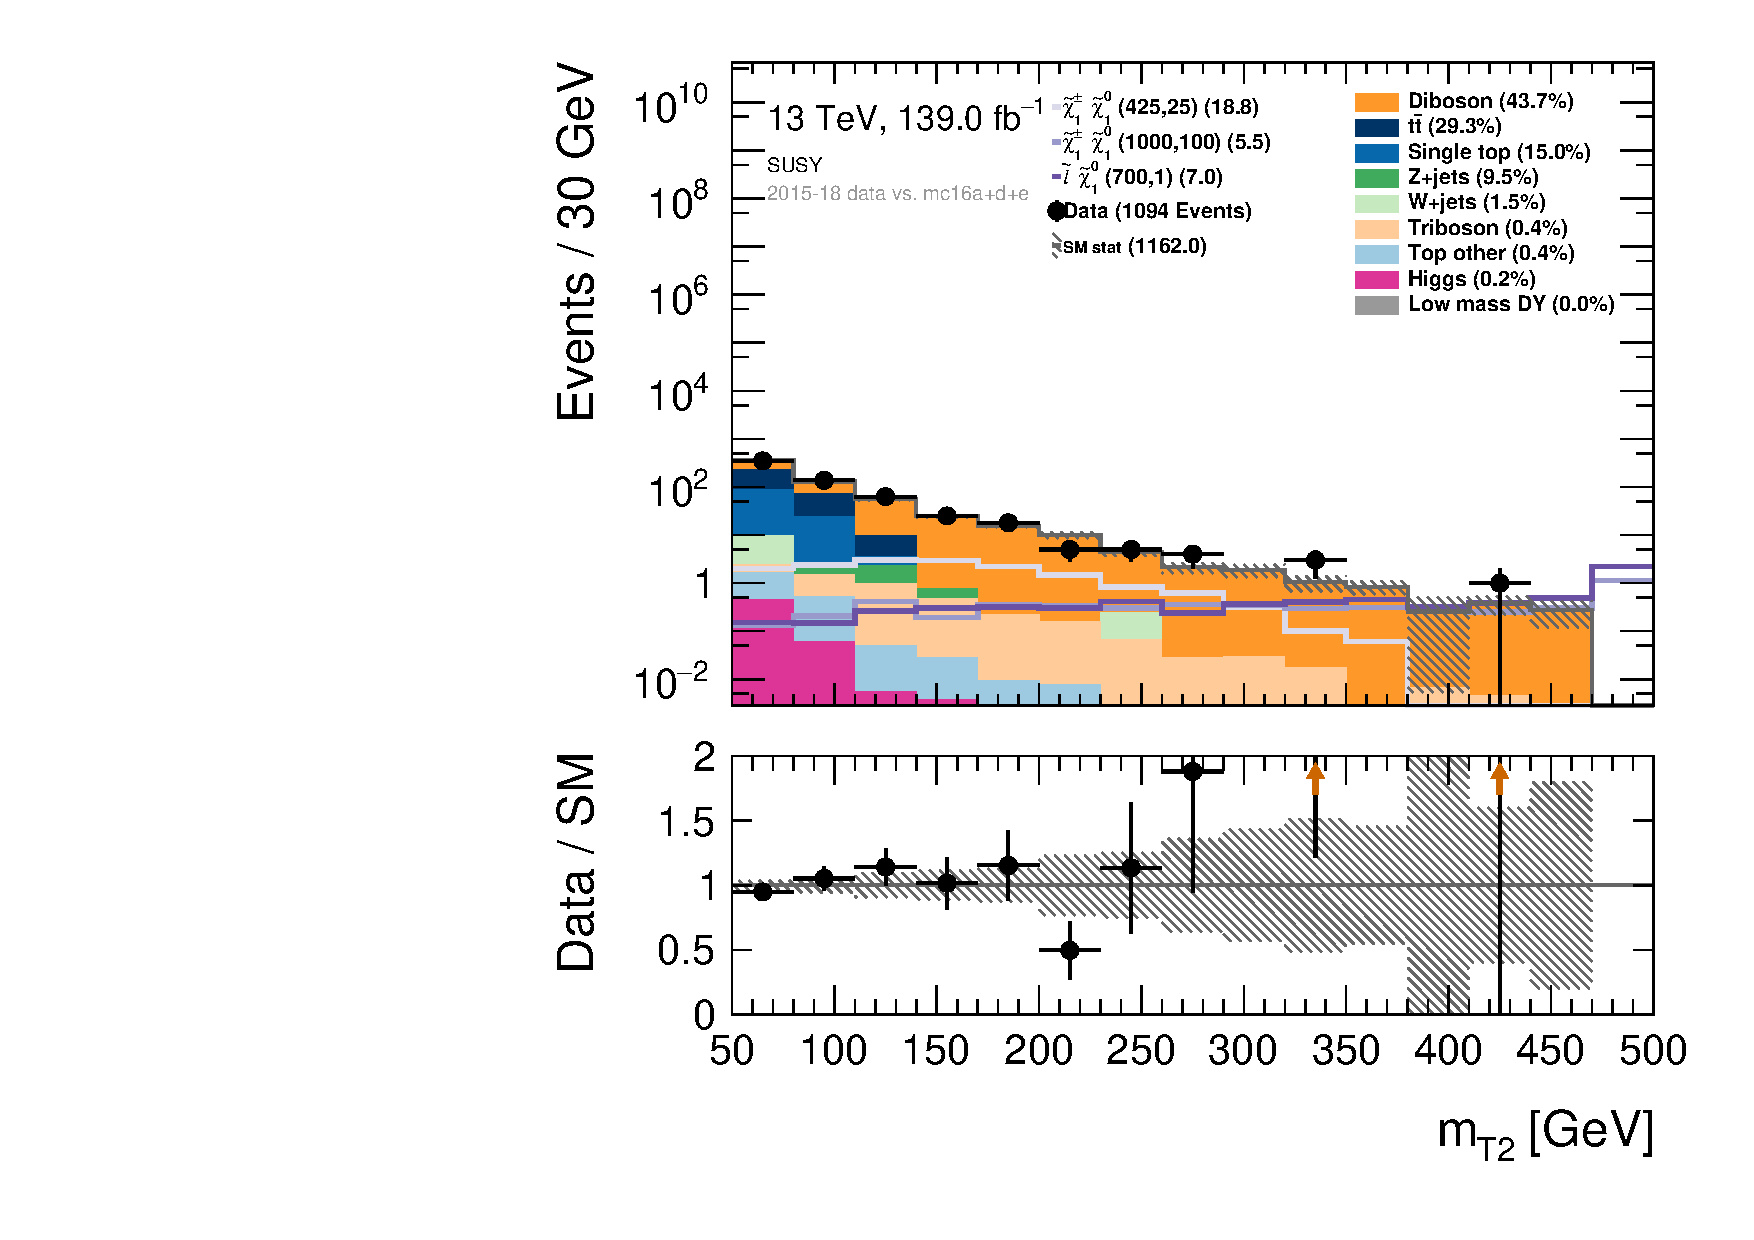
\includegraphics[width=0.5\textwidth]{Figures/SUSYcuts/hist1d_mt2_SUSY.pdf}
    \caption{Plot of the distribution of $m_{T2}$ after applying the cuts on MET significance.}
    \label{fig:stepsSUSY3}
\end{figure}

As we can see in figure \ref{fig:stepsSUSY1}-\ref{fig:stepsSUSY3} and table \ref{tab:cutflowSUSY}, the signal have been reduced, but not as much as all of the background contributions. This implies that we have been able to get rid of the background without affecting the signal too much, which also was our goal by doing this. 

\begin{landscape}
\begin{table}[H]
    \centering
    %\rotatebox{90}{
    \begin{tabular}{l l l l l l l}
    \toprule
    \textbf{Sample} & \textbf{OS+SF+2L} & \textbf{jet-veto} & $\mathbf{m_{ll}}$ & \textbf{MET} & \textbf{MET sign} & $\mathbf{m_{T_2}}$\\
    \midrule
    \midrule
        Drell-Yan & 733055.427 & 64177.536 & 40.384 & 0.000 & 0.000  & 0.000 \\
        Higgs & 1055360.610 & 442535.035 & 451.966 & 3.222 & 2.411 & 0.005\\
        Single top & 96745.087 & 7383.056 & 3313.872 & 283.960 & 174.644 & 0.000\\
        $t\Bar{t}$ & 948716.615 & 16272.119 & 7648.974 & 710.246 & 340.903 & 0.000\\
        Z+jets & 142460122.600 & 97803688.386 & 1273912.476 & 533.182 & 109.925 & -0.004\\
        Top other & 14730.742 & 120.671 & 56.003 & 8.079 & 4.353 & 0.034\\
        W+jets & 8978.117 & 3252.185 & 1359.621 & 58.245 & 17.834 & 0.182\\
        Triboson & 345.791 & 65.545 & 25.860 & 5.757 & 4.633 & 0.653\\
        Diboson & 355149.910 & 107329.899 & 24243.651 & 740.741 & 507.329 & 42.588\\
        Data & 148644251.000 & 99518352.000 & 1384140.000 & 2328.000 & 1094.000 & 40.000\\
        $(\Tilde{l}, \Tilde{\chi}_1^0) (700,1)$ & 22.710 & 8.692 & 8.519 & 7.873 & 6.987 & 6.062\\
        $(\Tilde{\chi}_1^\pm, \Tilde{\chi}_1^0) (1000, 100)$ & 16.475 & 6.546 & 6.355 & 5.997 & 5.468 & 4.347\\
        $(\Tilde{\chi}_1^\pm, \Tilde{\chi}_1^0) (425,25)$ & 90.581 & 40.109 & 30.305 & 20.816 & 18.756 & 6.692\\
    \bottomrule
    \end{tabular}
    %}
    \caption{A cut flow overview after applying the different cuts in table \ref{tab:cutsSUSY} with one signal sample from each of the three SUSY processes.}
    \label{tab:cutflowSUSY}
\end{table}
\end{landscape}




\begin{comment}


\newgeometry{twoside,inner=3cm,outer=2cm}
\begin{figure}[H]
%\begin{minipage}{2\textwidth}
%\begin{adjustwidth}{-3cm}{-3cm}
\centering
%\advance\leftskip-4cm 
%\advance\rightskip-4cm 
    \begin{subfigure}[t!]{0.49\textwidth}
        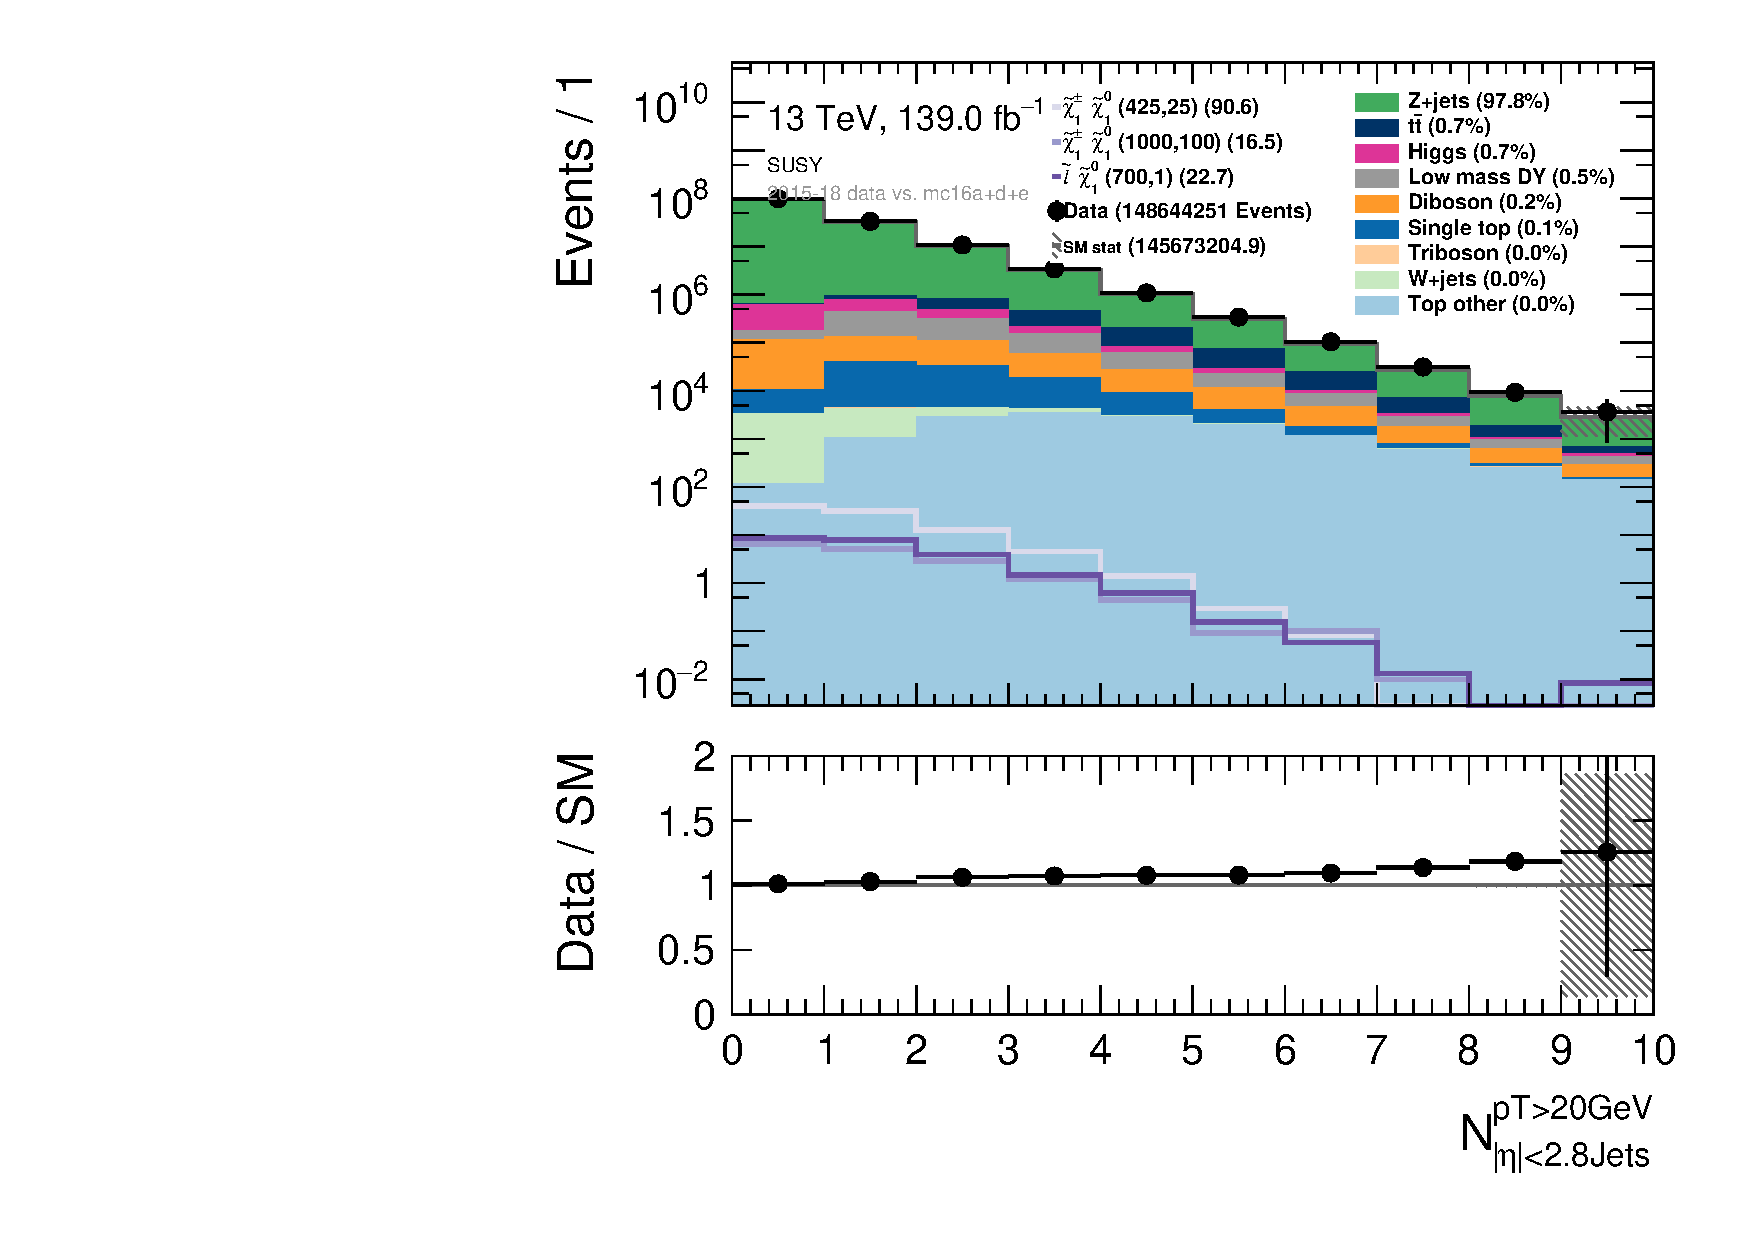
\includegraphics[width=\textwidth]{Figures/SUSYcuts/hist1d_nJet20_SUSY.pdf}
    \caption{Stransverse mass for direct slepton production.}
    \label{fig:my_label}
    \end{subfigure}
    \begin{subfigure}[t!]{0.49\textwidth}
        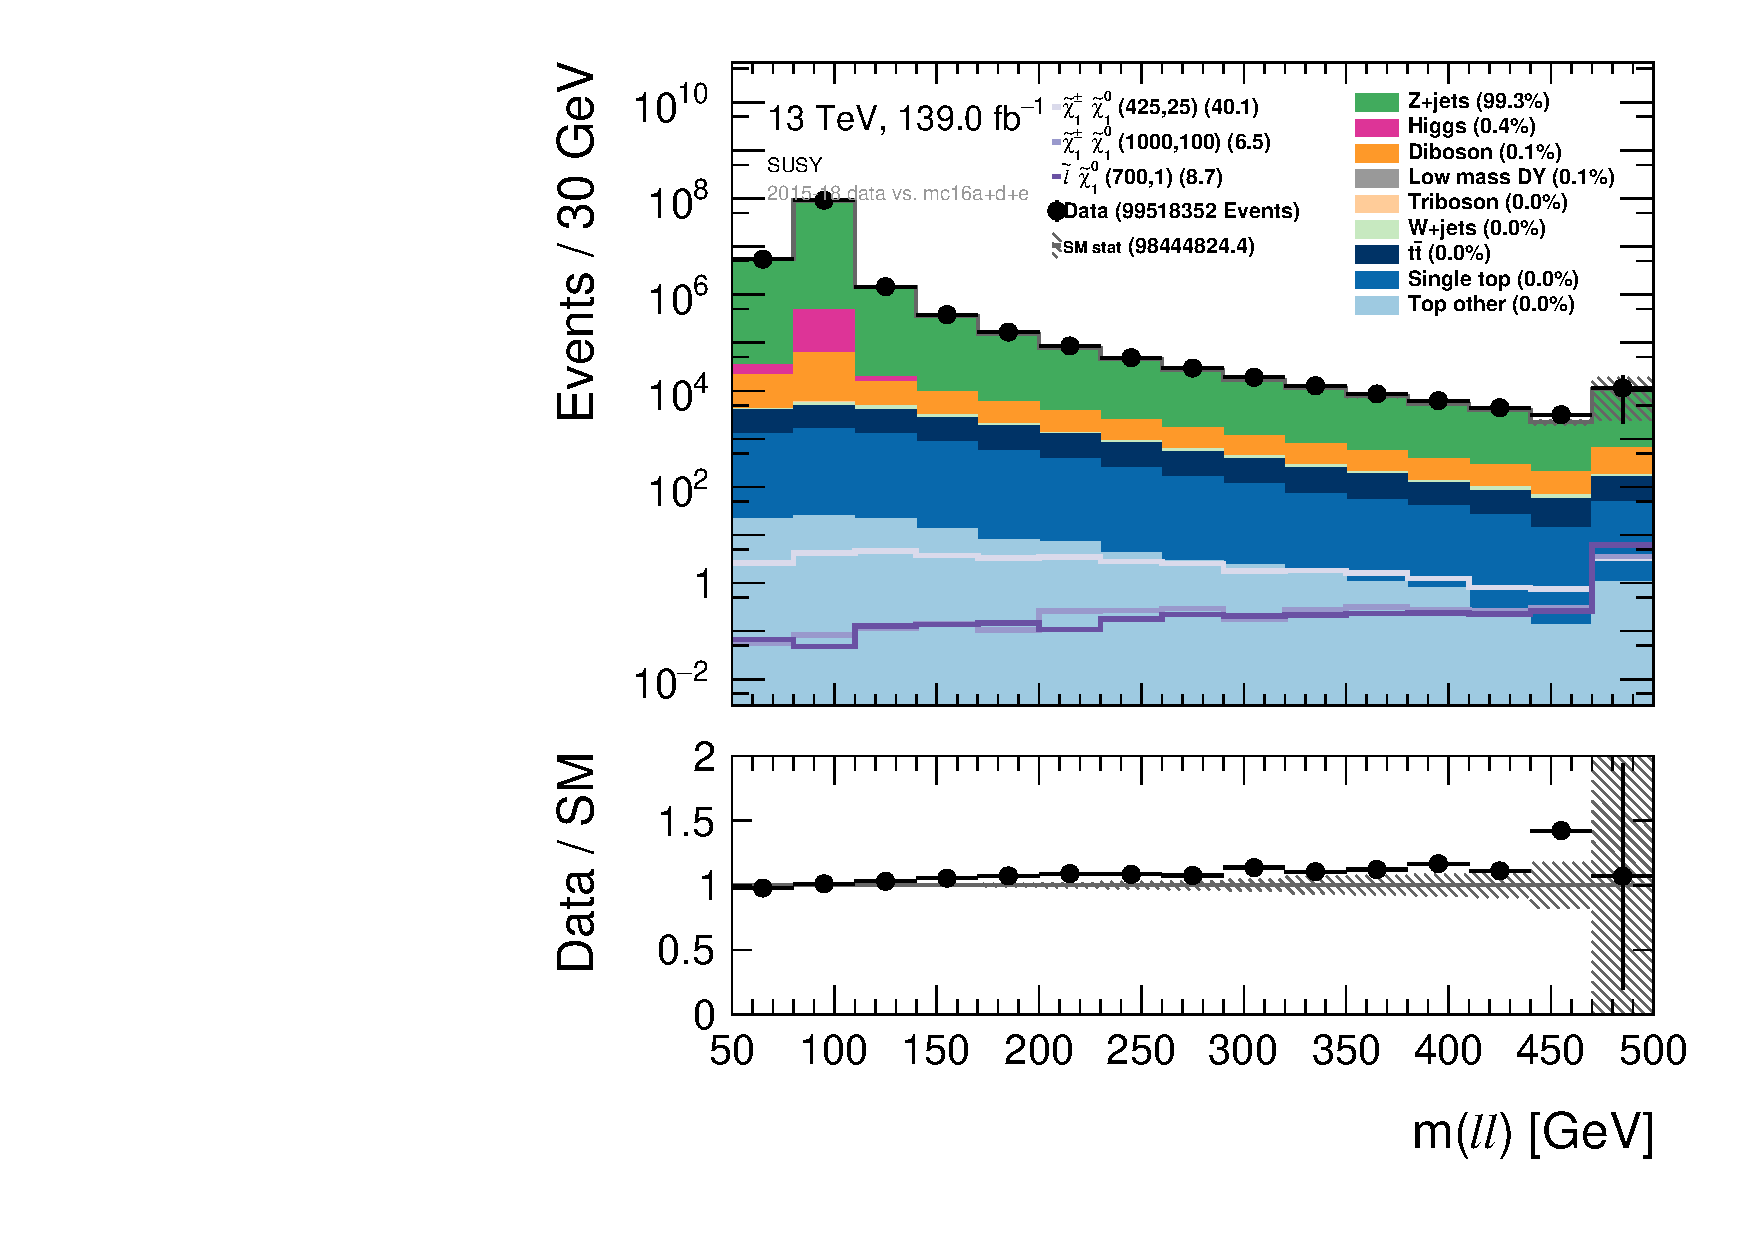
\includegraphics[width=\textwidth]{Figures/SUSYcuts/hist1d_mll_SUSY.pdf}
    \caption{Stransverse mass for chargino production via $\Tilde{l}/\Tilde{\nu}$.}
    \label{fig:my_label}
    \end{subfigure}
    \\
    \begin{subfigure}[t!]{0.49\textwidth}
        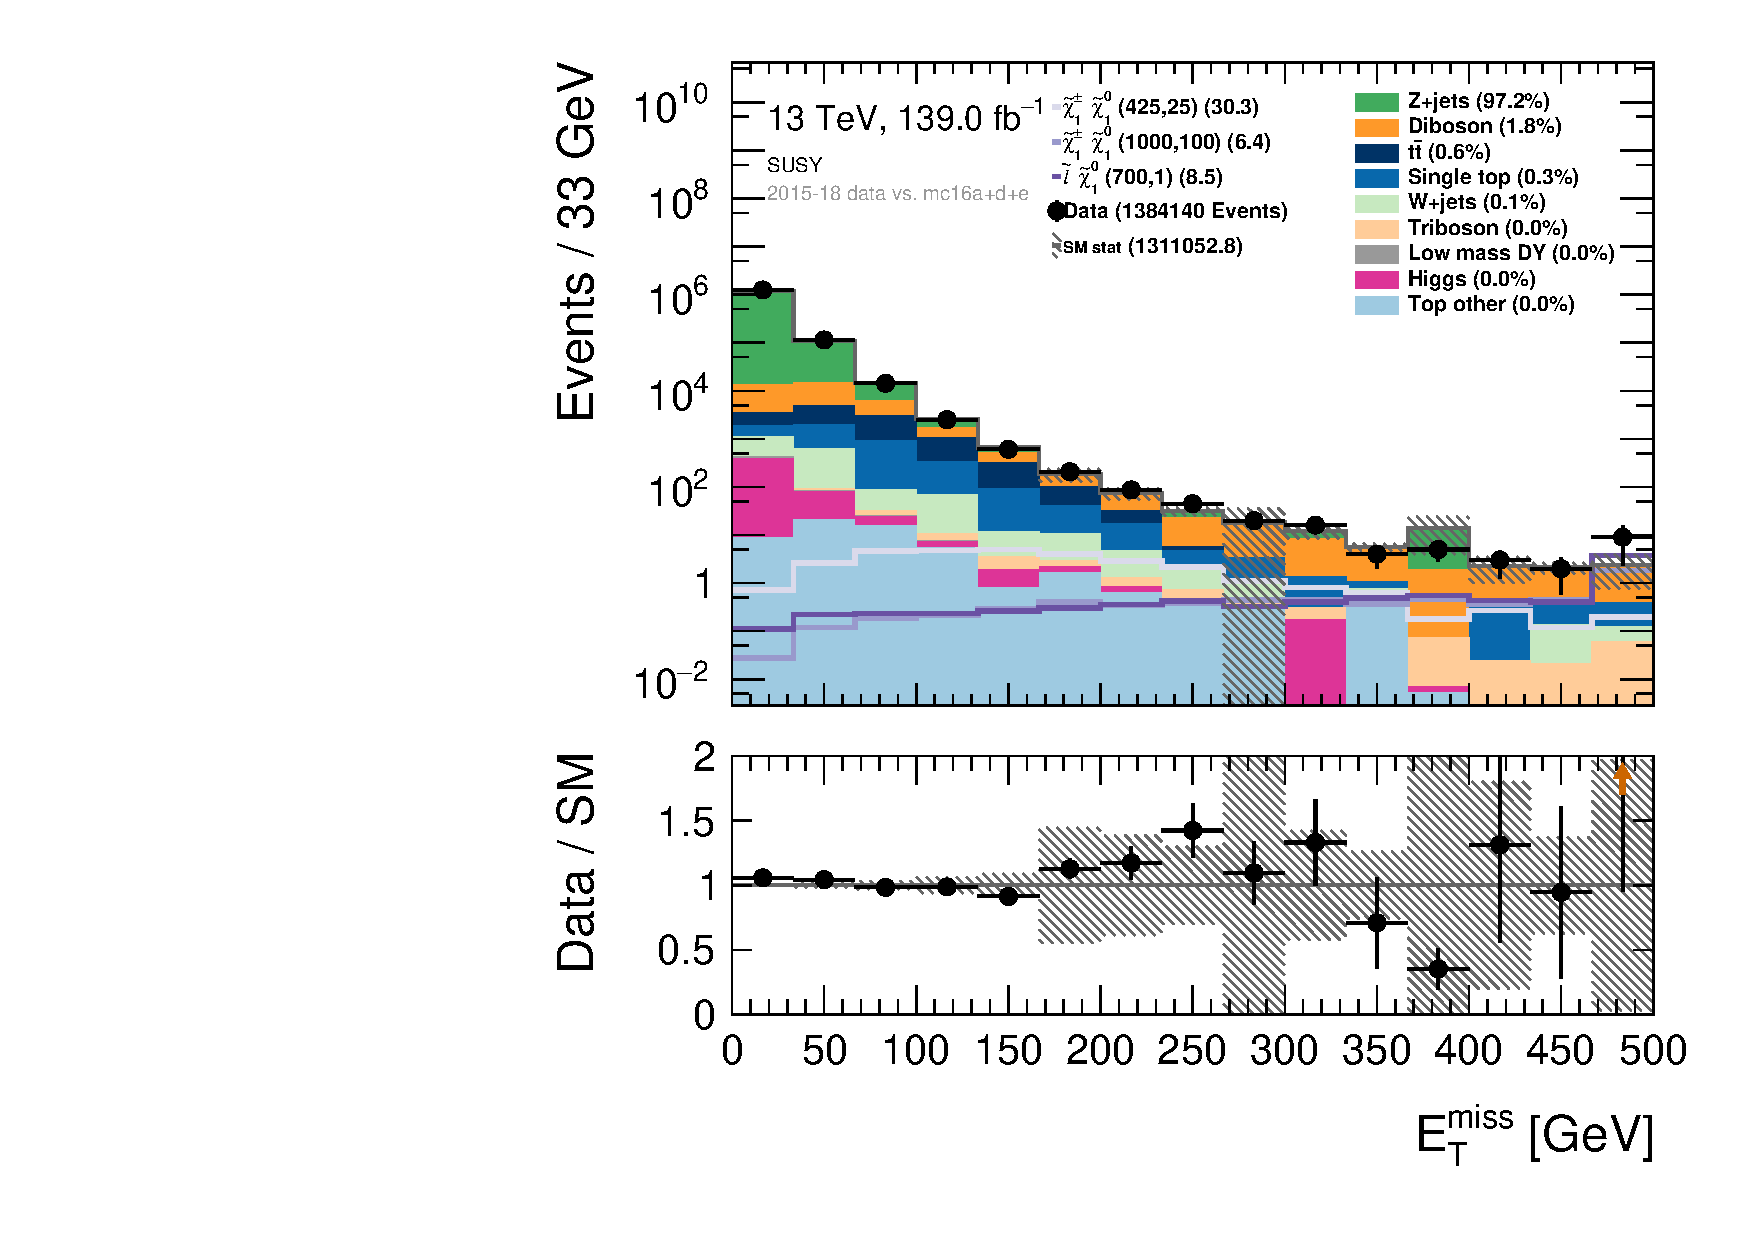
\includegraphics[width=\textwidth]{Figures/SUSYcuts/hist1d_met_Et_SUSY.pdf}
    \caption{Stransverse mass for chargino production via $W^\pm$.}
    \label{fig:my_label}
    \end{subfigure}
    \begin{subfigure}[t!]{0.49\textwidth}
        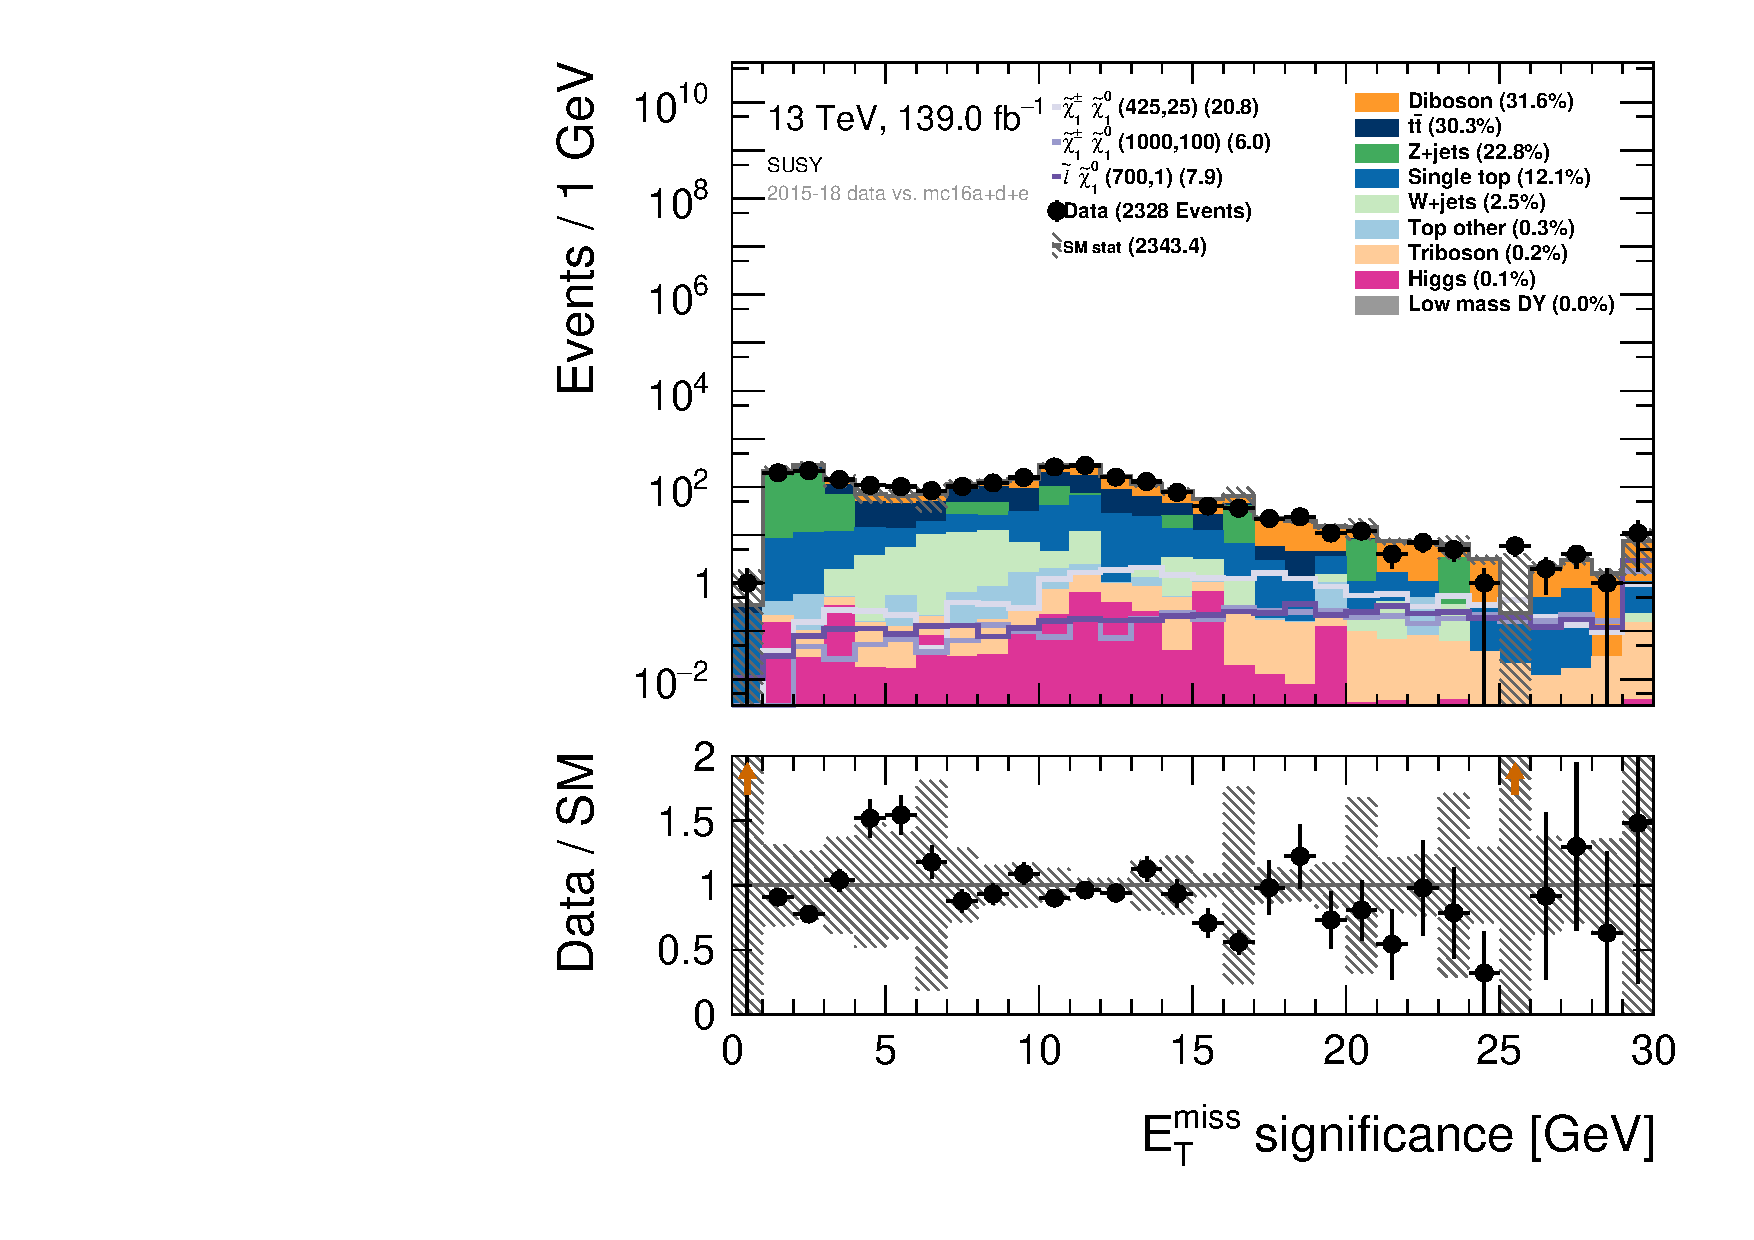
\includegraphics[width=\textwidth]{Figures/SUSYcuts/hist1d_met_Sign_SUSY.pdf}
    \caption{Missing transverse energy for mono-Z.}
    \label{fig:my_label}
    \end{subfigure}
    \\
    \begin{subfigure}[t!]{0.49\textwidth}
        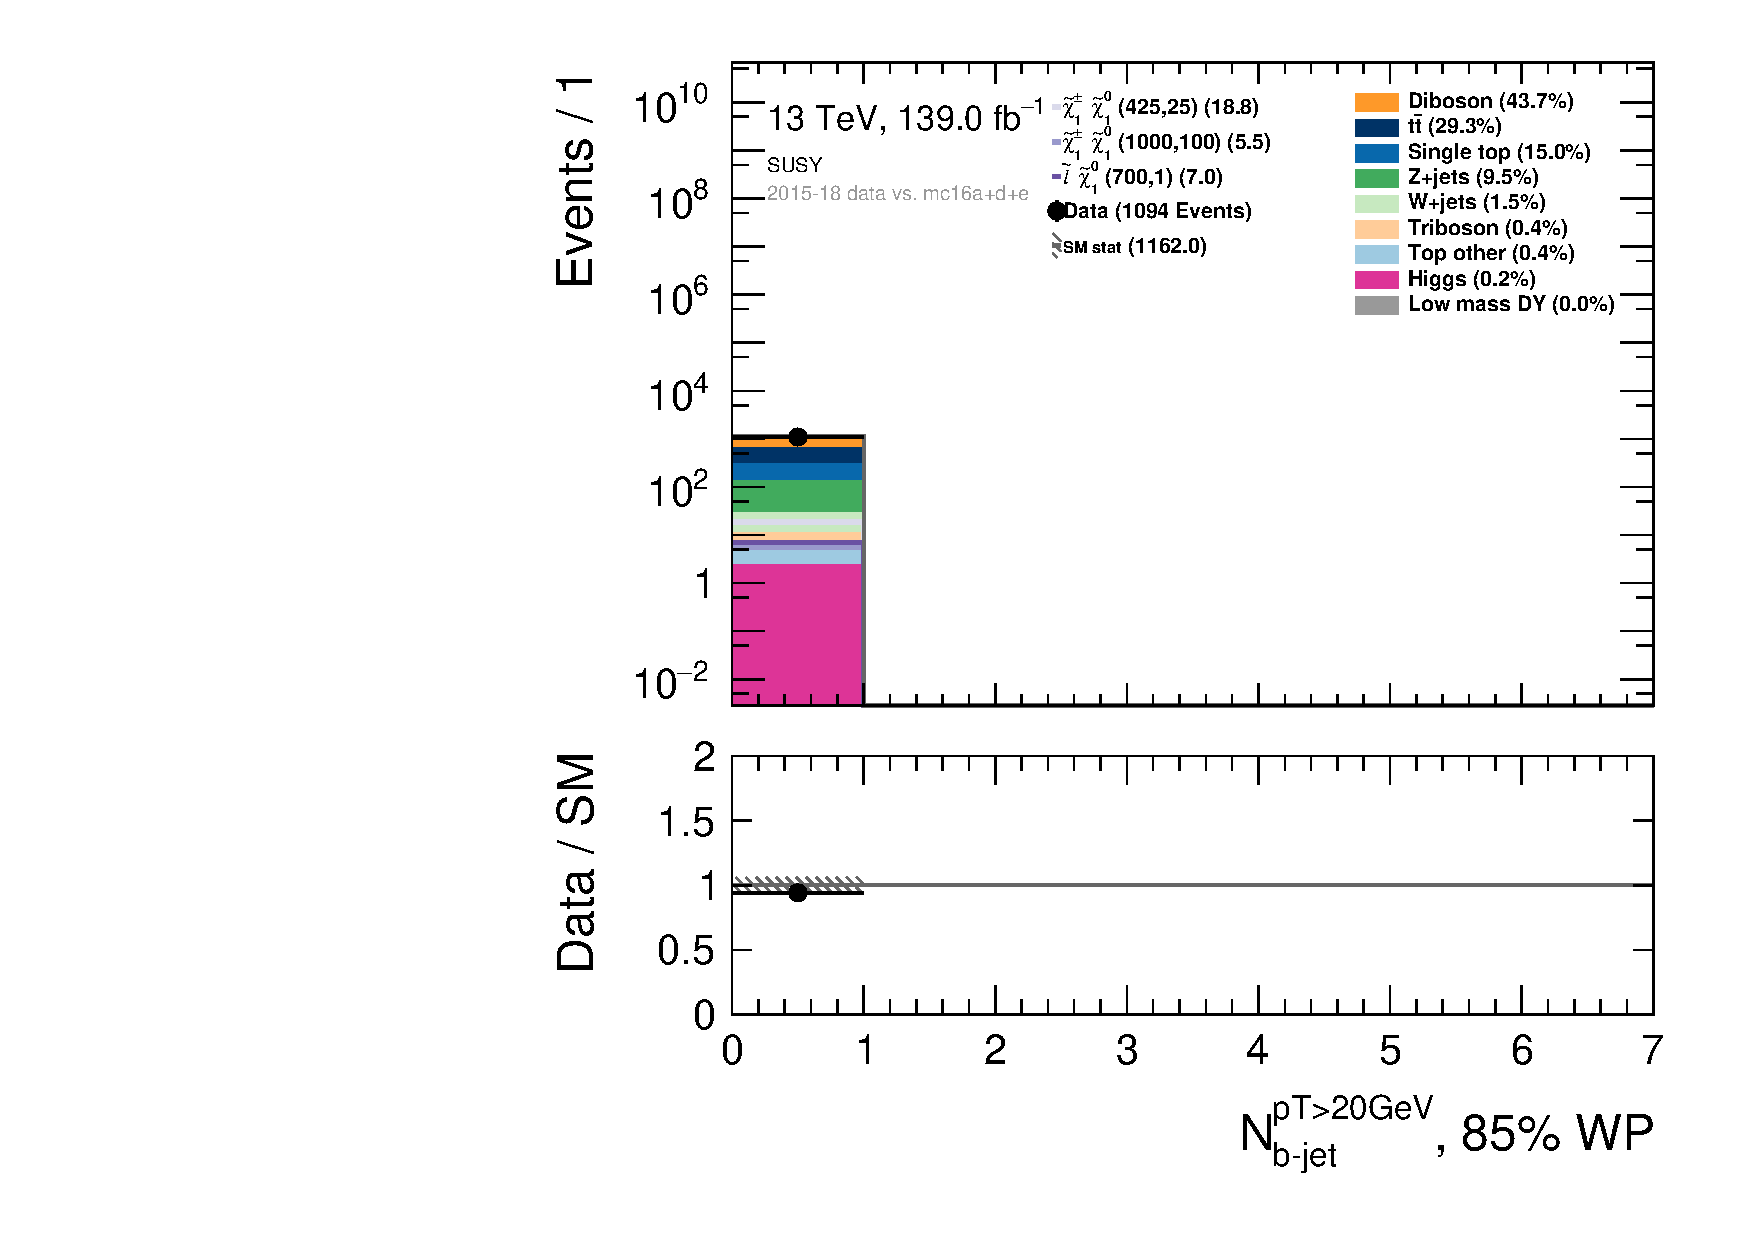
\includegraphics[width=\textwidth]{Figures/SUSYcuts/hist1d_nBJet20_MV2c10_FixedCutBEff_85_SUSY.pdf}
    \caption{Stransverse mass for chargino production via $W^\pm$.}
    \label{fig:my_label}
    \end{subfigure}
    \begin{subfigure}[t!]{0.49\textwidth}
        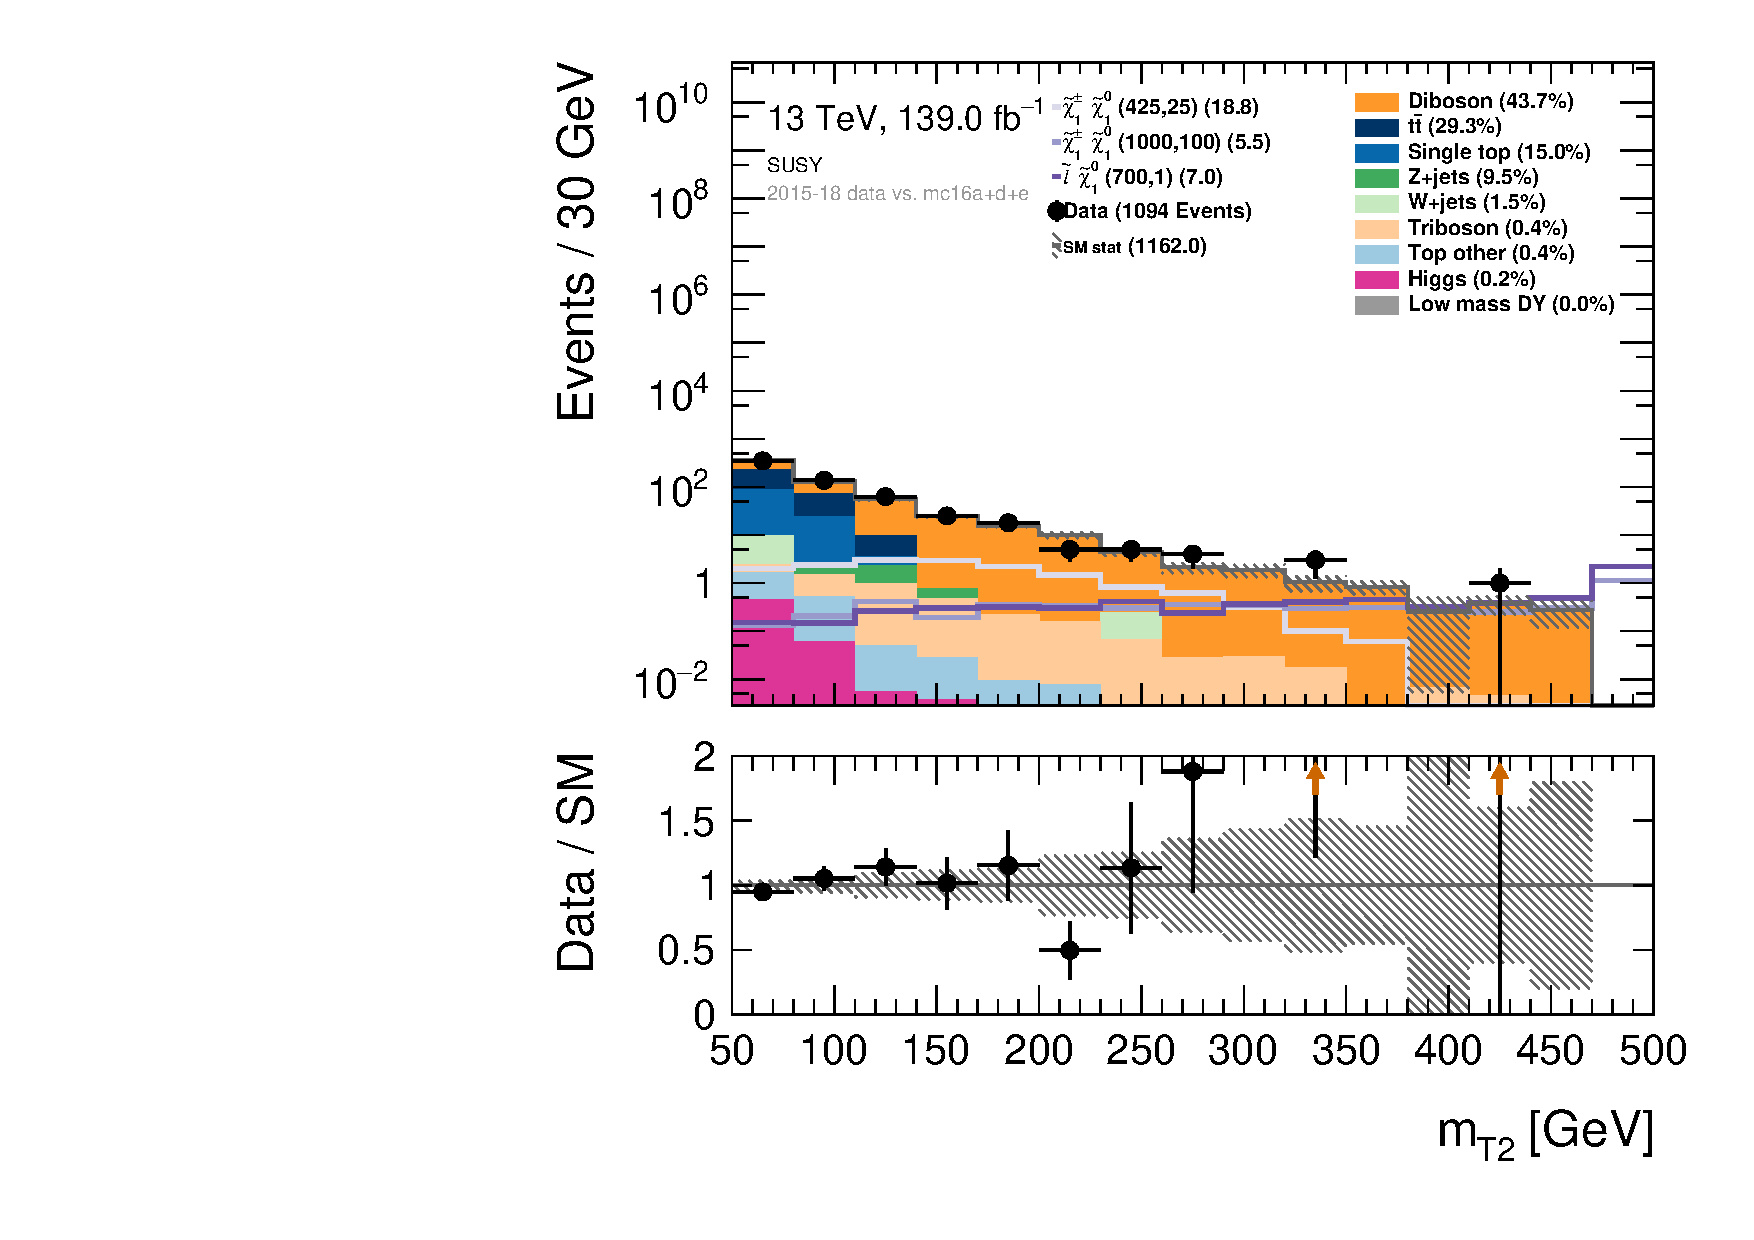
\includegraphics[width=\textwidth]{Figures/SUSYcuts/hist1d_mt2_SUSY.pdf}
    \caption{Missing transverse energy for mono-Z.}
    \label{fig:my_label}
    \end{subfigure}
    \caption{Plot of the four most important variables in direct slepton production with a cut on only two leptons with opposite charge in the final state.}
    \label{fig:cutandcountStepsSUSY}
\end{figure}
\restoregeometry
\end{comment}

















The same procedure was done for the mono-Z process, where we have applied the cuts from table \ref{tab:cutsDM} and we can see how much each cut affect the different contributions in table \ref{tab:cutflowDM}. 


\begin{table}[H]
    \centering
    \begin{tabular}{l l}\toprule
    \textbf{Variables} & \textbf{Cuts}\\
    \midrule
    \midrule
    Two leptons     &  OS with leading (subleading) $p_T >$ 30 (20) GeV\\
    $m_{ll}$     & 76 $< m_{ll} <$ 106 GeV\\
    $E_T^{miss}$ & $>$ 90 GeV\\
    $E_T^{miss}/H_T$ & $>$ 0.6\\
    $\Delta \phi (\Vec{p}_T^{ll}, E_T^{miss})$ & $>$ 2.7 radians\\
    $\Delta R_{ll}$ & $<$ 1.8\\
    Fractional $p_T$ difference & $|p_T^{ll} - p_T^{miss, jets}|/p_T^{ll} <$ 0.2\\
    b-jets & 0\\
    \bottomrule
     \end{tabular}
    \caption{Cuts added in the cut and count analysis taken from the publication for the mono-Z process \cite{monoZexclusion}.}
    \label{tab:cutsDM}
\end{table}

For the DM process, we have applied the cuts in table \ref{tab:cutsDM}, where we, as for the SUSY processes, demand to only have two leptons with opposite sign in the final state together with missing transverse energy. In addition to the cut on number of leptons, we cut on the $p_T$ of the leptons, for both the leading and subleading lepton. The cut on the subleading lepton will not affect anything because it is already done a cut at 25 GeV while handling the data for this thesis. This is shown in figure \ref{fig:mllDM} and table \ref{tab:cutflowDM}, where we can see that the distribution looks very similar as for the SUSY processes earlier in this chapter. We have demanded to have a Z-boson which we can see the results from in figure \ref{fig:metDM}. For both these cuts, we can see that Z+jets are the dominating background, where all the different backgrounds are reduced. 

\begin{figure}[H]
    \centering
    \begin{subfigure}[t!]{0.49\textwidth}
        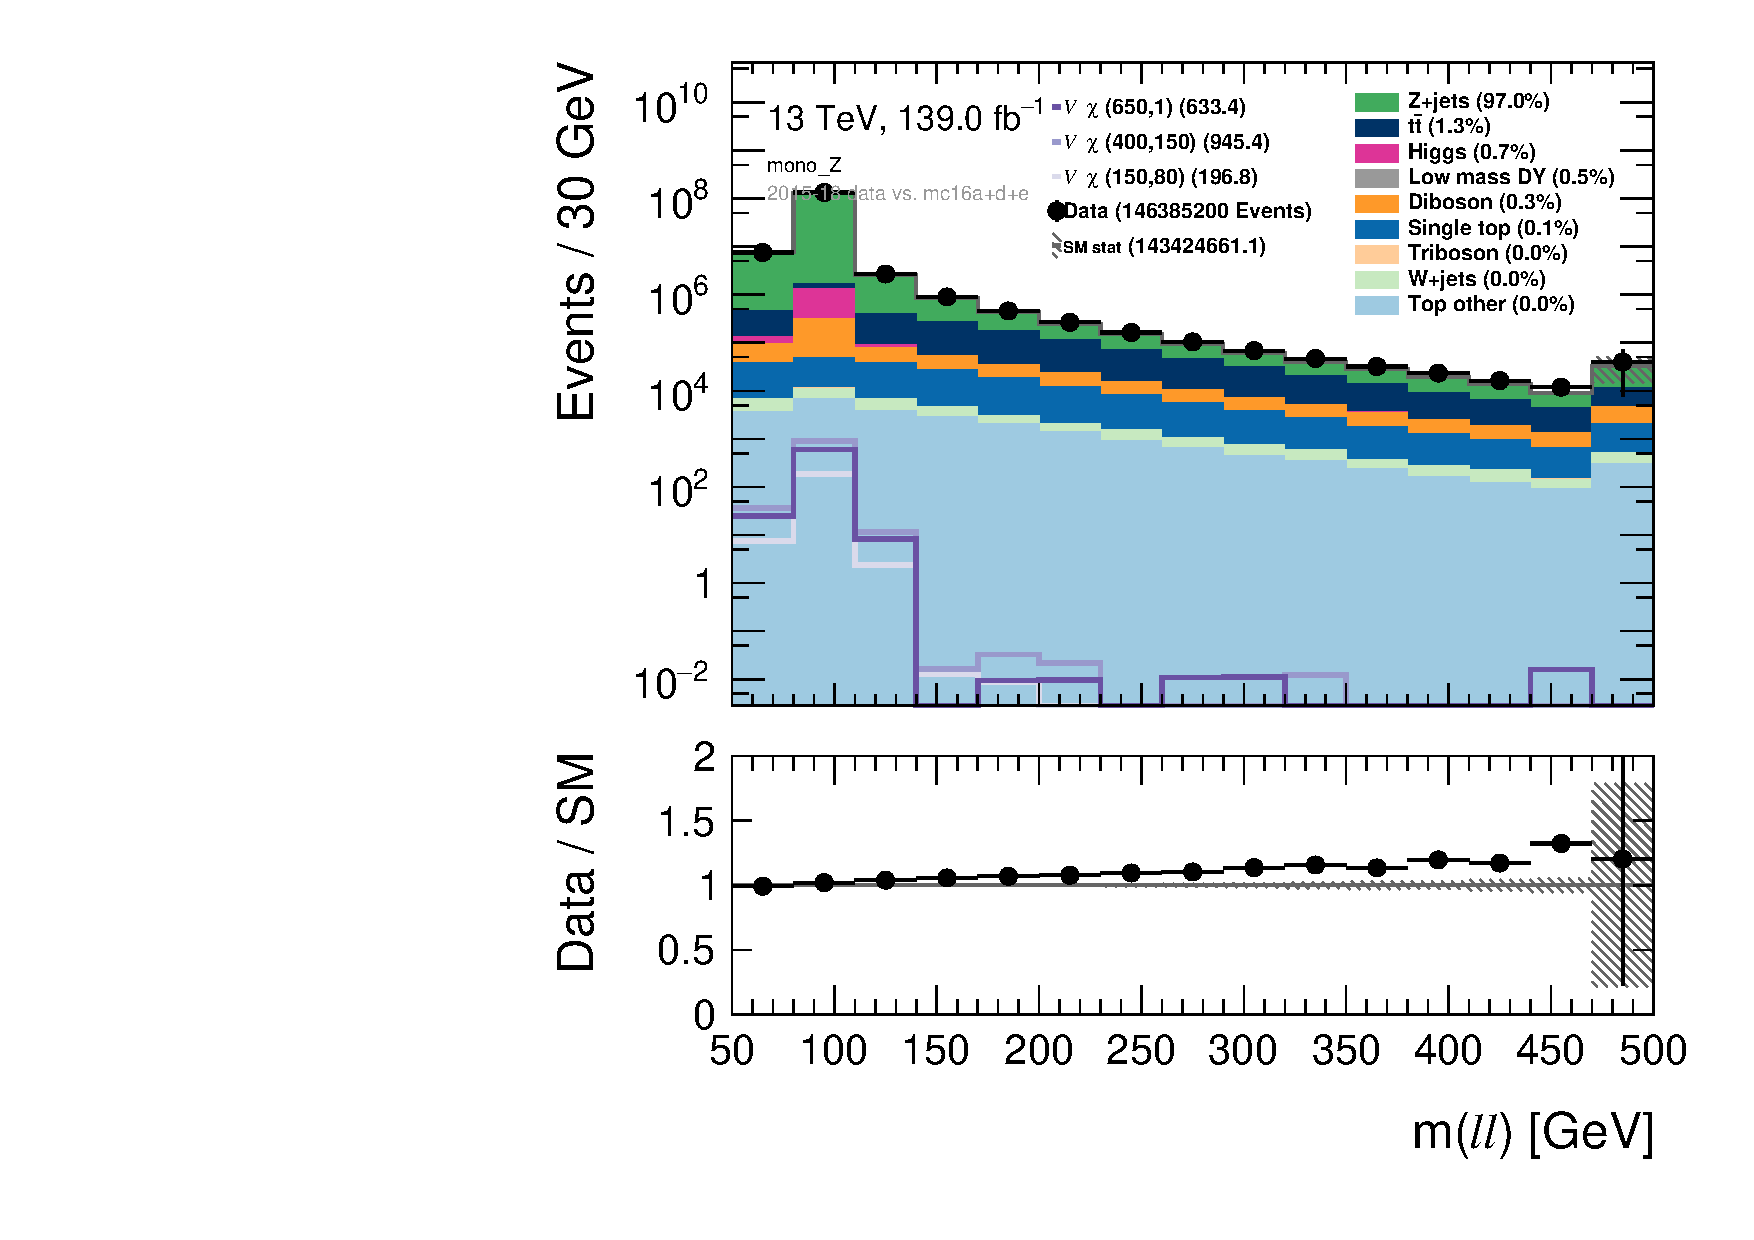
\includegraphics[width=\textwidth]{Figures/MonoZcuts/hist1d_mll_mono_Z.pdf}
    \caption{Invariant mass.}
    \label{fig:mllDM}
    \end{subfigure}
    \begin{subfigure}[t!]{0.49\textwidth}
        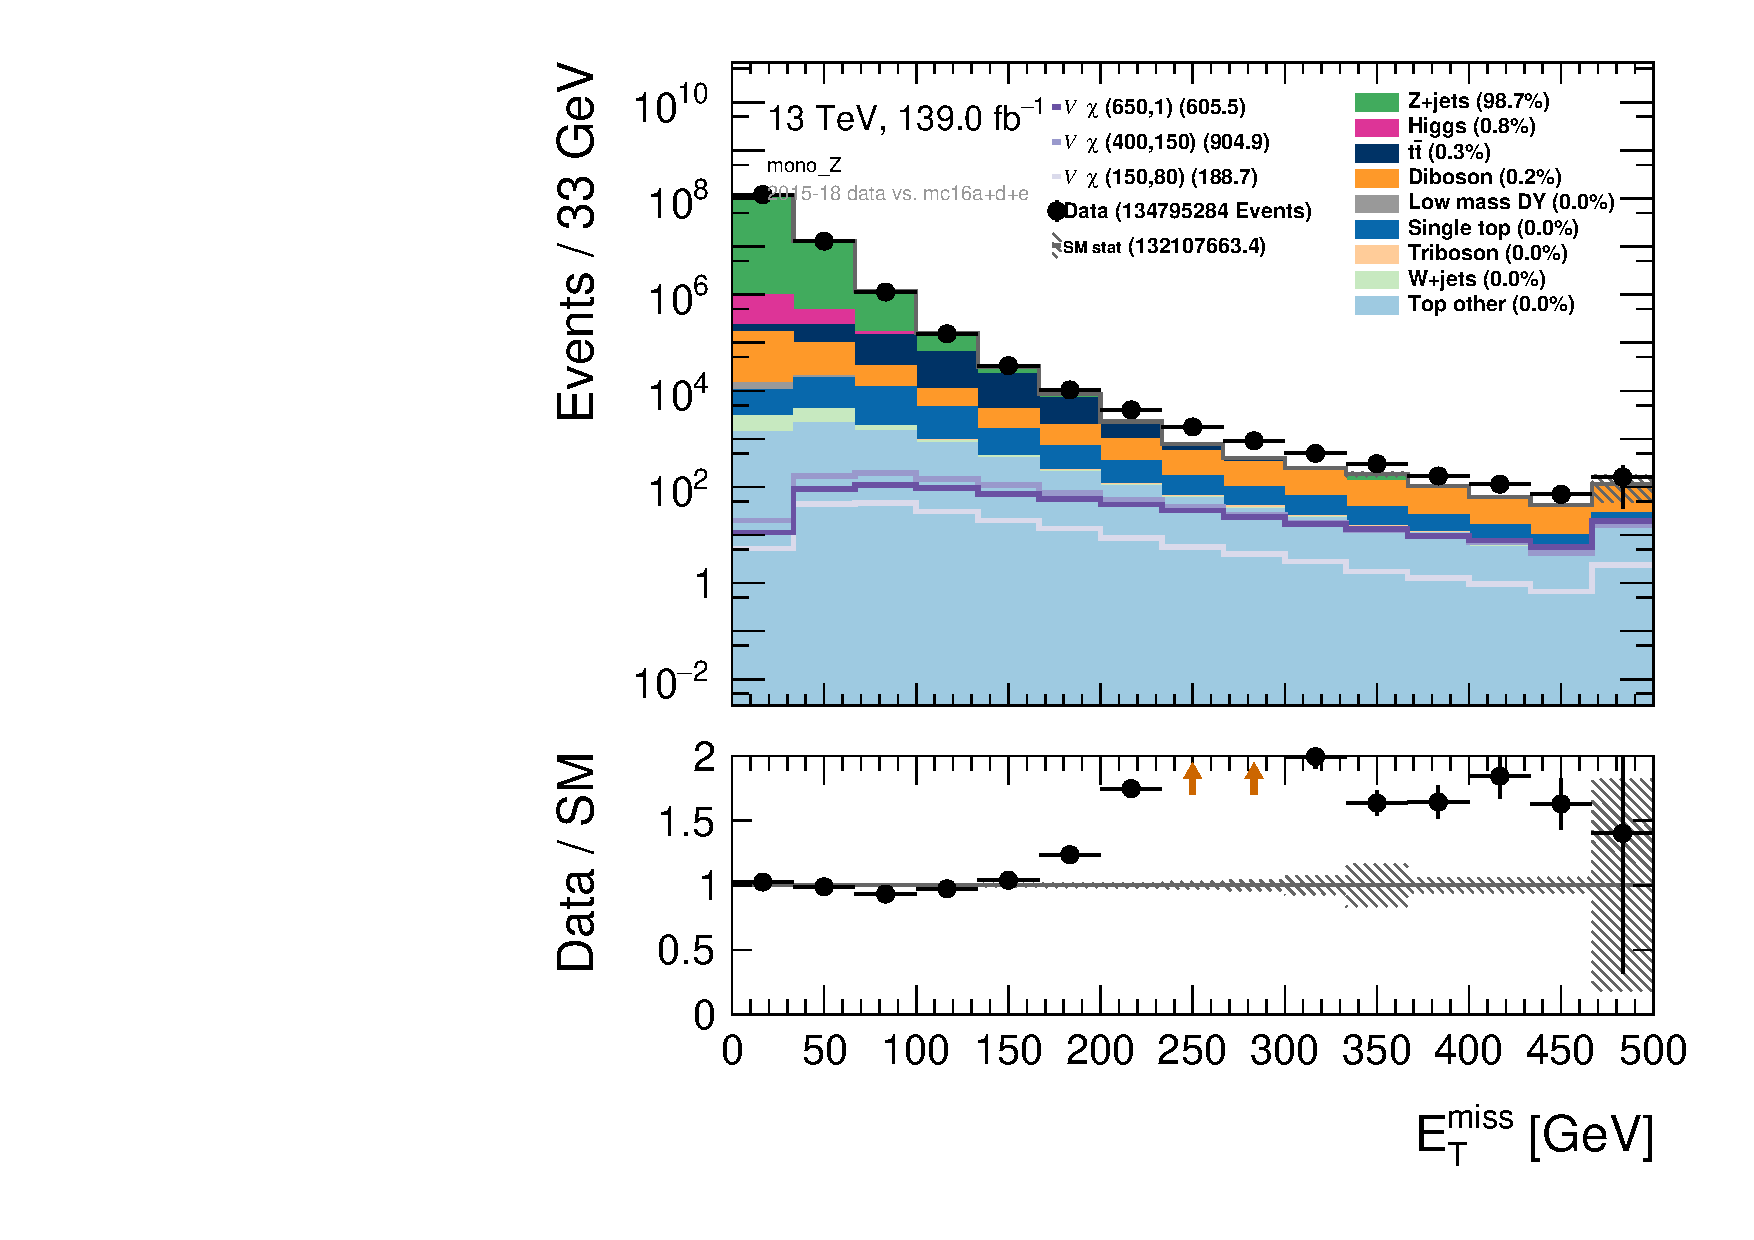
\includegraphics[width=\textwidth]{Figures/MonoZcuts/hist1d_met_Et_mono_Z_1.pdf}
    \caption{Missing transverse energy.}
    \label{fig:metDM}
    \end{subfigure}
    \caption{Plot of different distributions after applying the cuts on 2L, OS, $p_T$ of the two leptons (a) and invariant mass (b).}
    \label{fig:stepsDM1}
\end{figure}

We also do a slightly more gentle cut on the missing transverse energy for this process than the SUSY processes because we have several other MET dependent variables for mono-Z. One of these are $E_T^{miss}/H_T$. After applying the MET cut, we can see that the Z+jets are less dominating, but since the MET/$H_T$ reduces the $t\Bar{t}$ background, the Z+jets becomes more dominating again. The results are shown in figure \ref{fig:stepsDM2}.

\begin{figure}[H]
    \centering
    \begin{subfigure}[t!]{0.49\textwidth}
        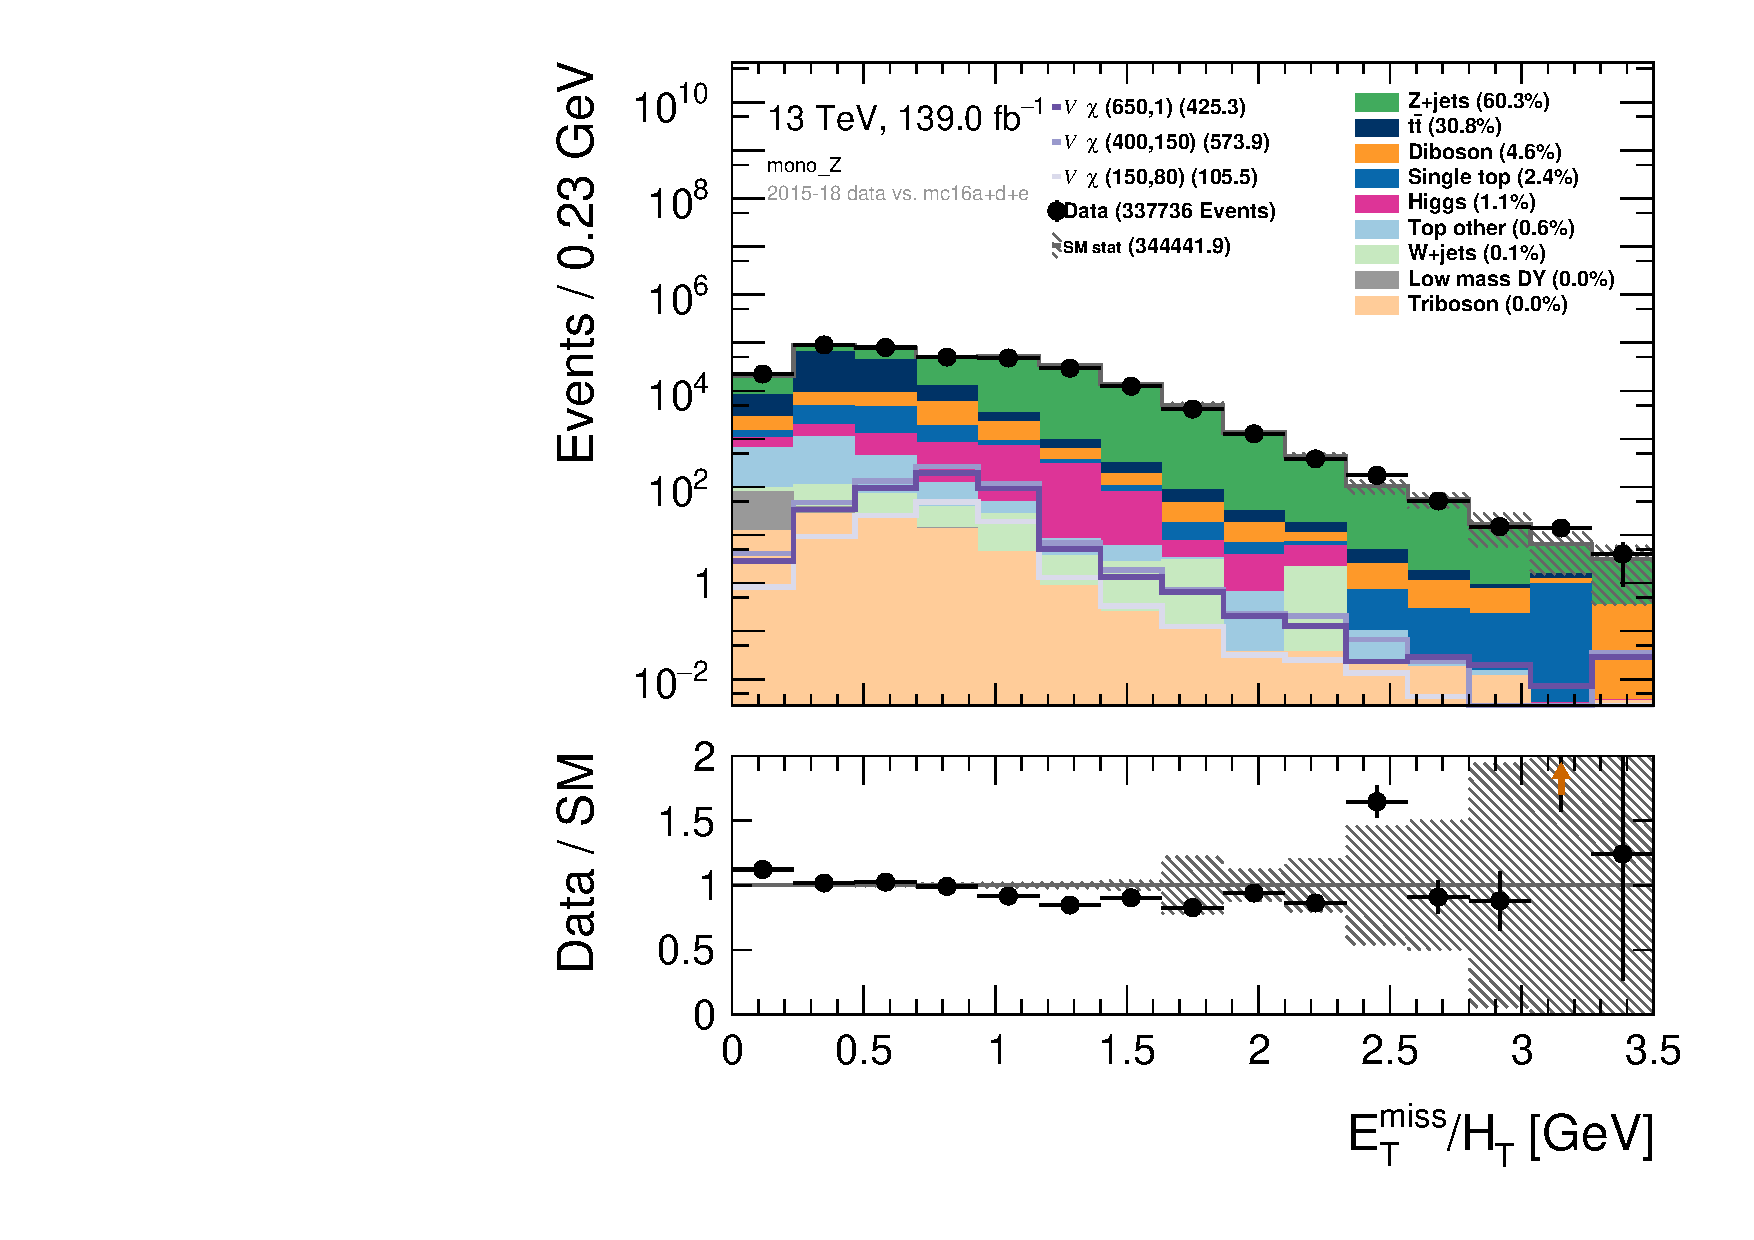
\includegraphics[width=\textwidth]{Figures/MonoZcuts/hist1d_met_HT_mono_Z.pdf}
    \caption{The ratio between $E_T^{miss}$ and $H_T$.}
    \label{fig:metHTDM}
    \end{subfigure}
    \begin{subfigure}[t!]{0.49\textwidth}
        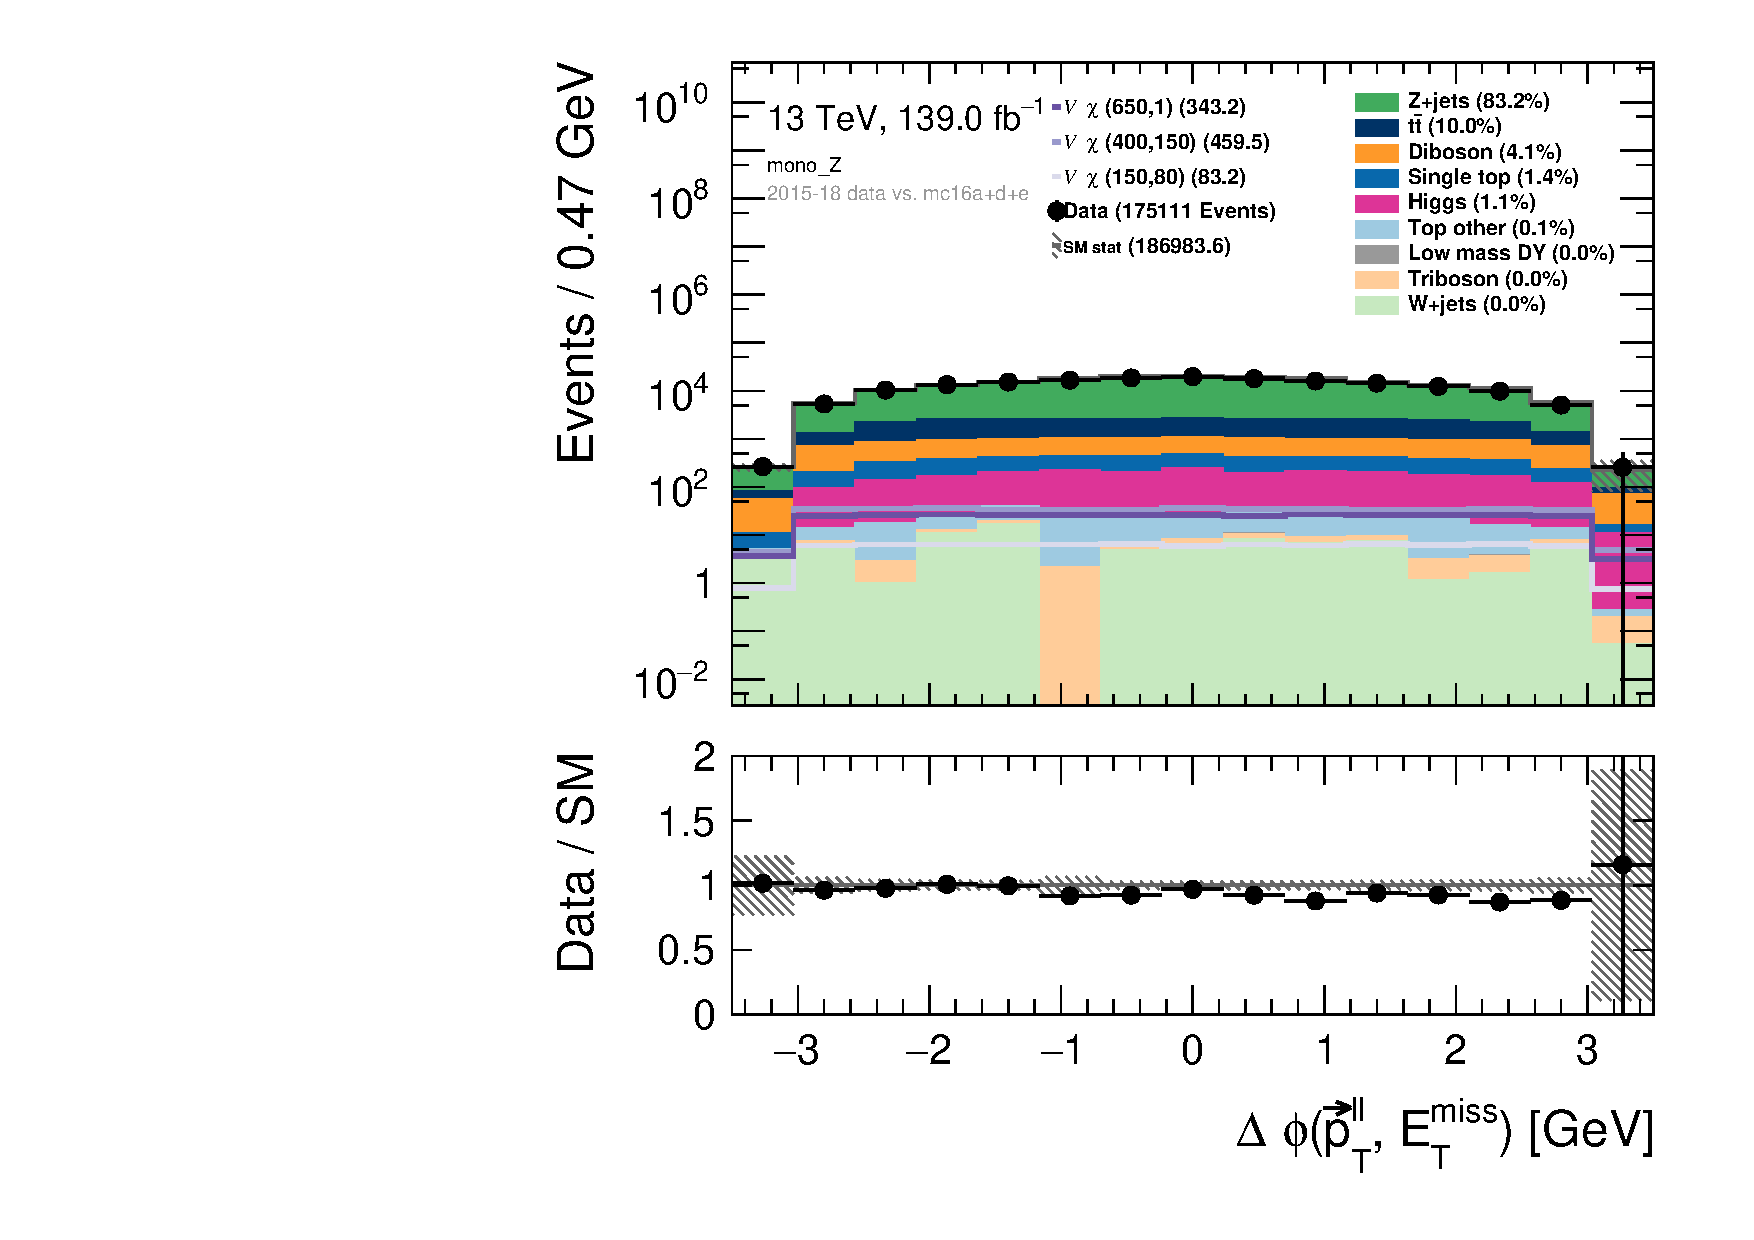
\includegraphics[width=\textwidth]{Figures/MonoZcuts/hist1d_deltaPhi_mono_Z.pdf}
    \caption{The azimuthal angle difference between the dilepton system and $E_T^{miss}$.}
    \label{fig:delphiDM}
    \end{subfigure}
    \caption{Plot of different distributions after applying the cuts on MET (a) and MET/$H_T$ (b).}
    \label{fig:stepsDM2}
\end{figure}


The next cut that is applied is $\Delta \phi (\Vec{p}_T^{ll}, E_T^{miss})$, where the two leptons also have to be close to each other, which can be demanded by $\Delta R_{ll}$. $\Delta \phi$ is also one of the MET dependent variables we have used for the mono-Z process. The results after applying these cuts are presented in figure \ref{fig:stepsDM3} and as we can see, the Z+jets keeps being the dominating background. 




\begin{figure}[H]
    \centering
    \begin{subfigure}[t!]{0.49\textwidth}
        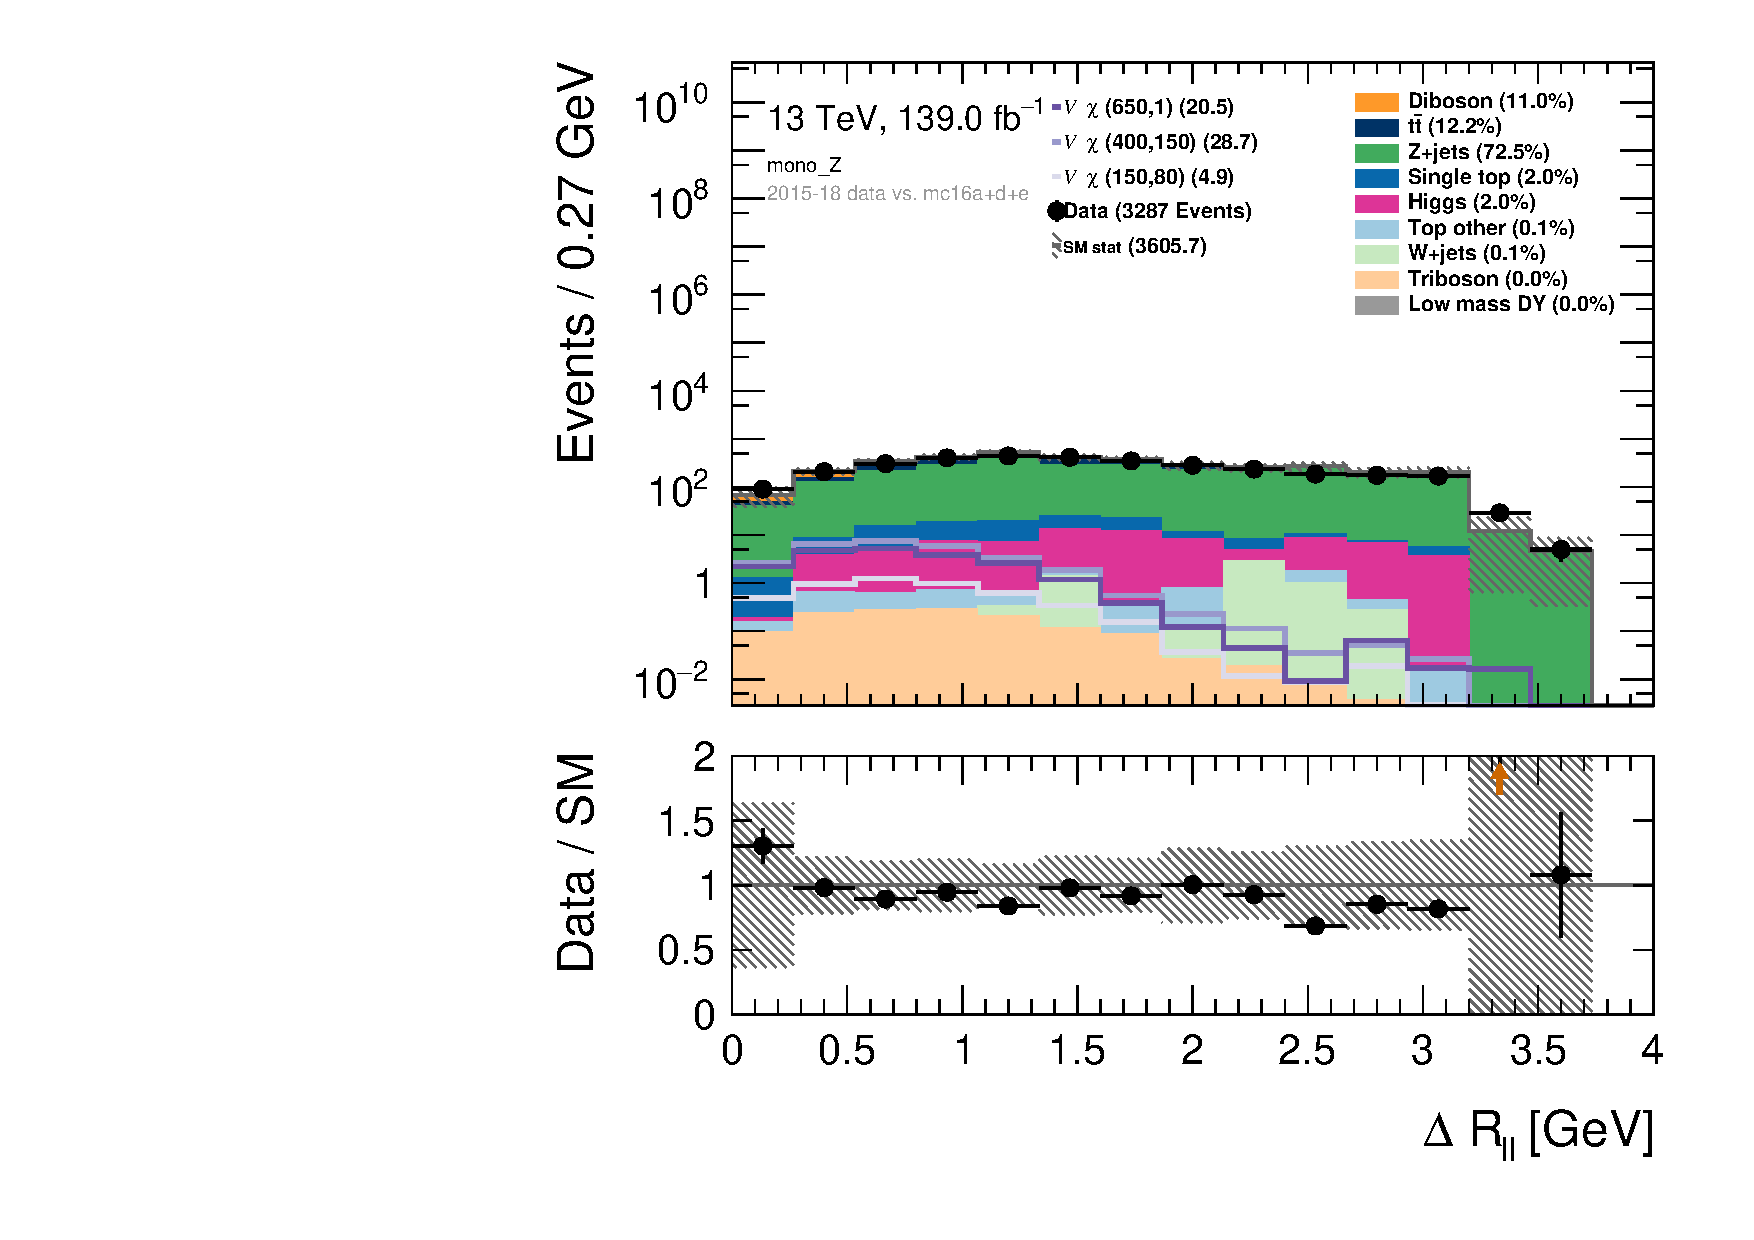
\includegraphics[width=\textwidth]{Figures/MonoZcuts/hist1d_deltaRll_mono_Z.pdf}
    \caption{Distance between the two leptons.}
    \label{fig:delRllDM}
    \end{subfigure}
    \begin{subfigure}[t!]{0.49\textwidth}
        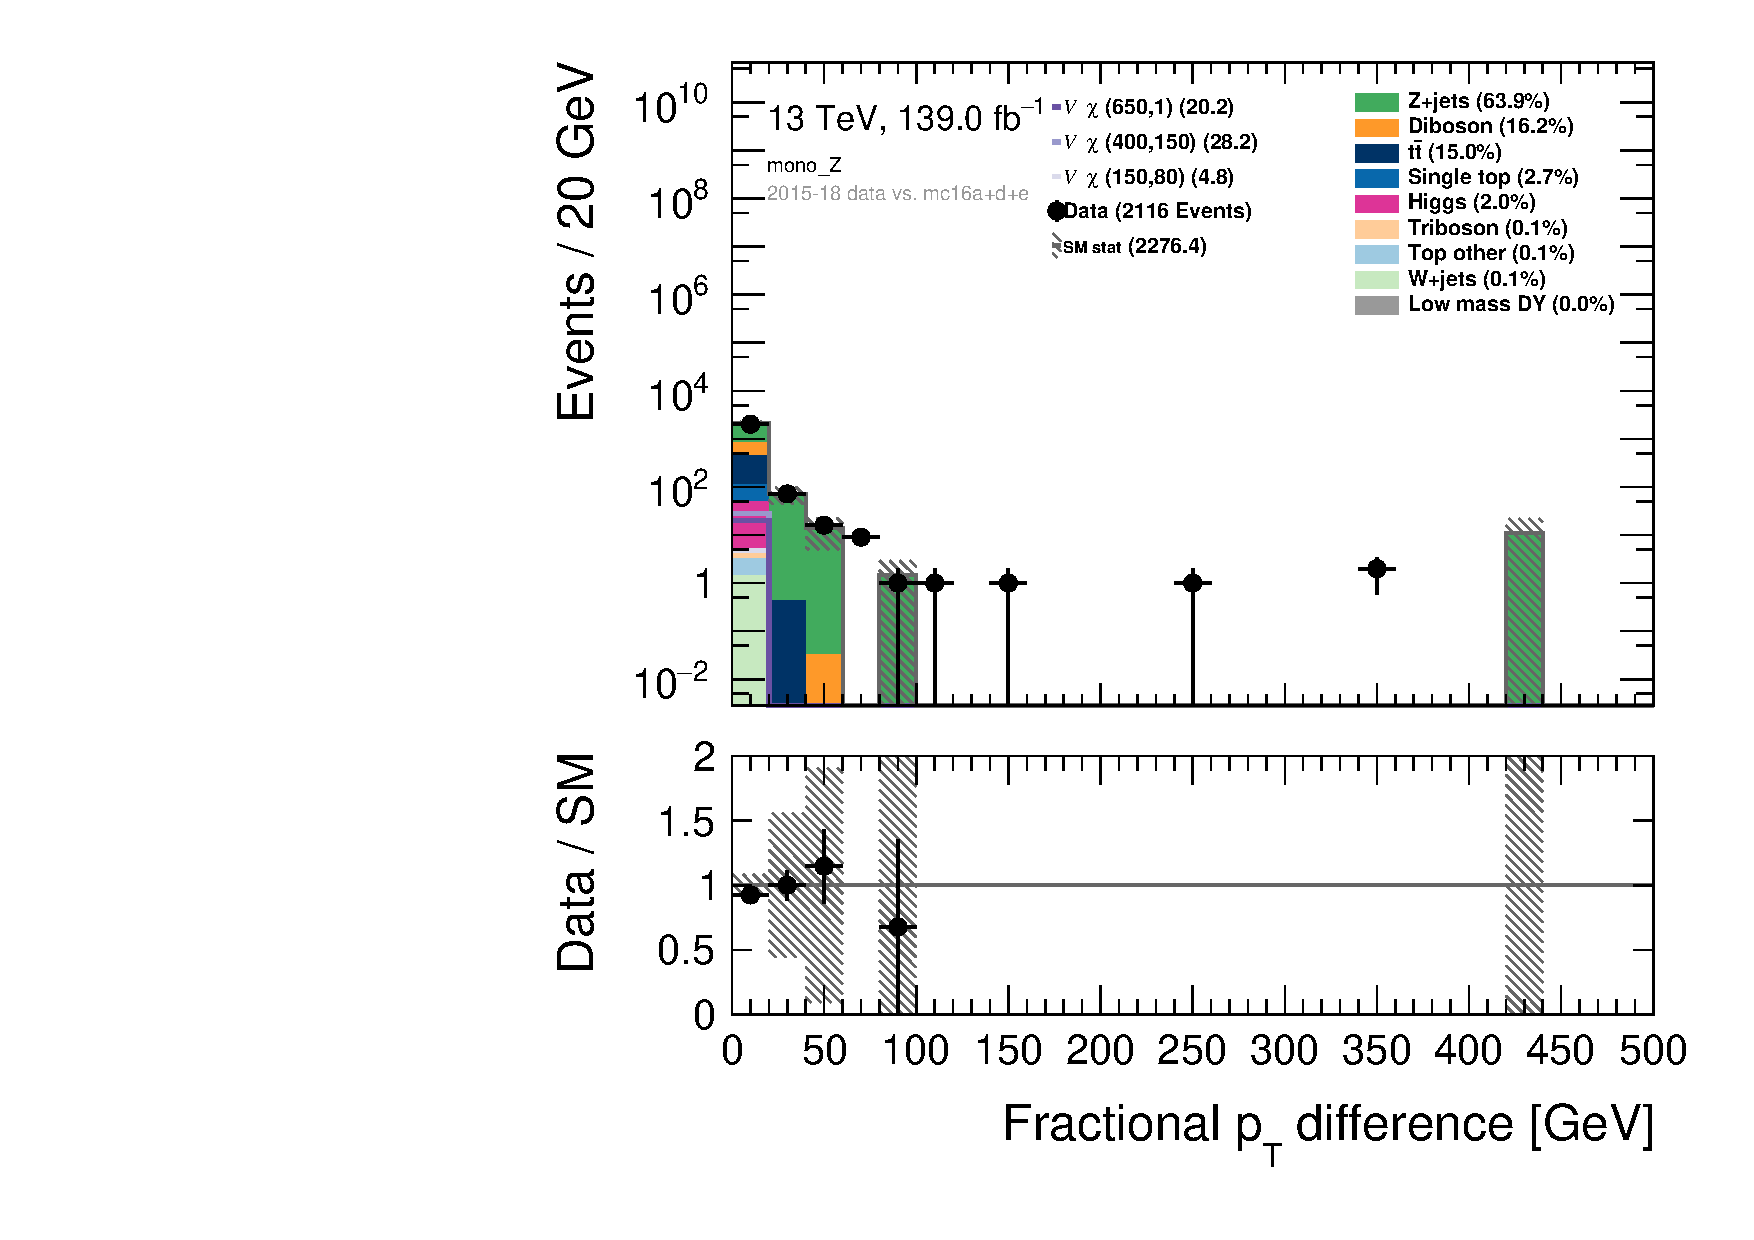
\includegraphics[width=\textwidth]{Figures/MonoZcuts/hist1d_pTdiff_mono_Z.pdf}
    \caption{The difference between the dilepton $p_T$, the selected jets $p_T$ and the vector sum of $\Vec{E}_T^{miss}$.}
    \label{fig:pTdiffDM}
    \end{subfigure}
    \caption{Plot of different distributions after applying the cuts on $\Delta \phi$ (a) and $\Delta R_{ll}$ (b).}
    \label{fig:stepsDM3}
\end{figure}


The last cuts we apply are on the fractional $p_T$ difference and a b-jet veto. The results from adding the $p_T$ cut are presented in figure \ref{fig:stepsDM4}, while the final results including b-jet veto is presented in figure \ref{fig:cutandcountMONA} later in this section. We can also see for both these cases that the dominating background have become diboson, which is the same as for the SUSY processes. 

\begin{figure}[H]
    \centering
        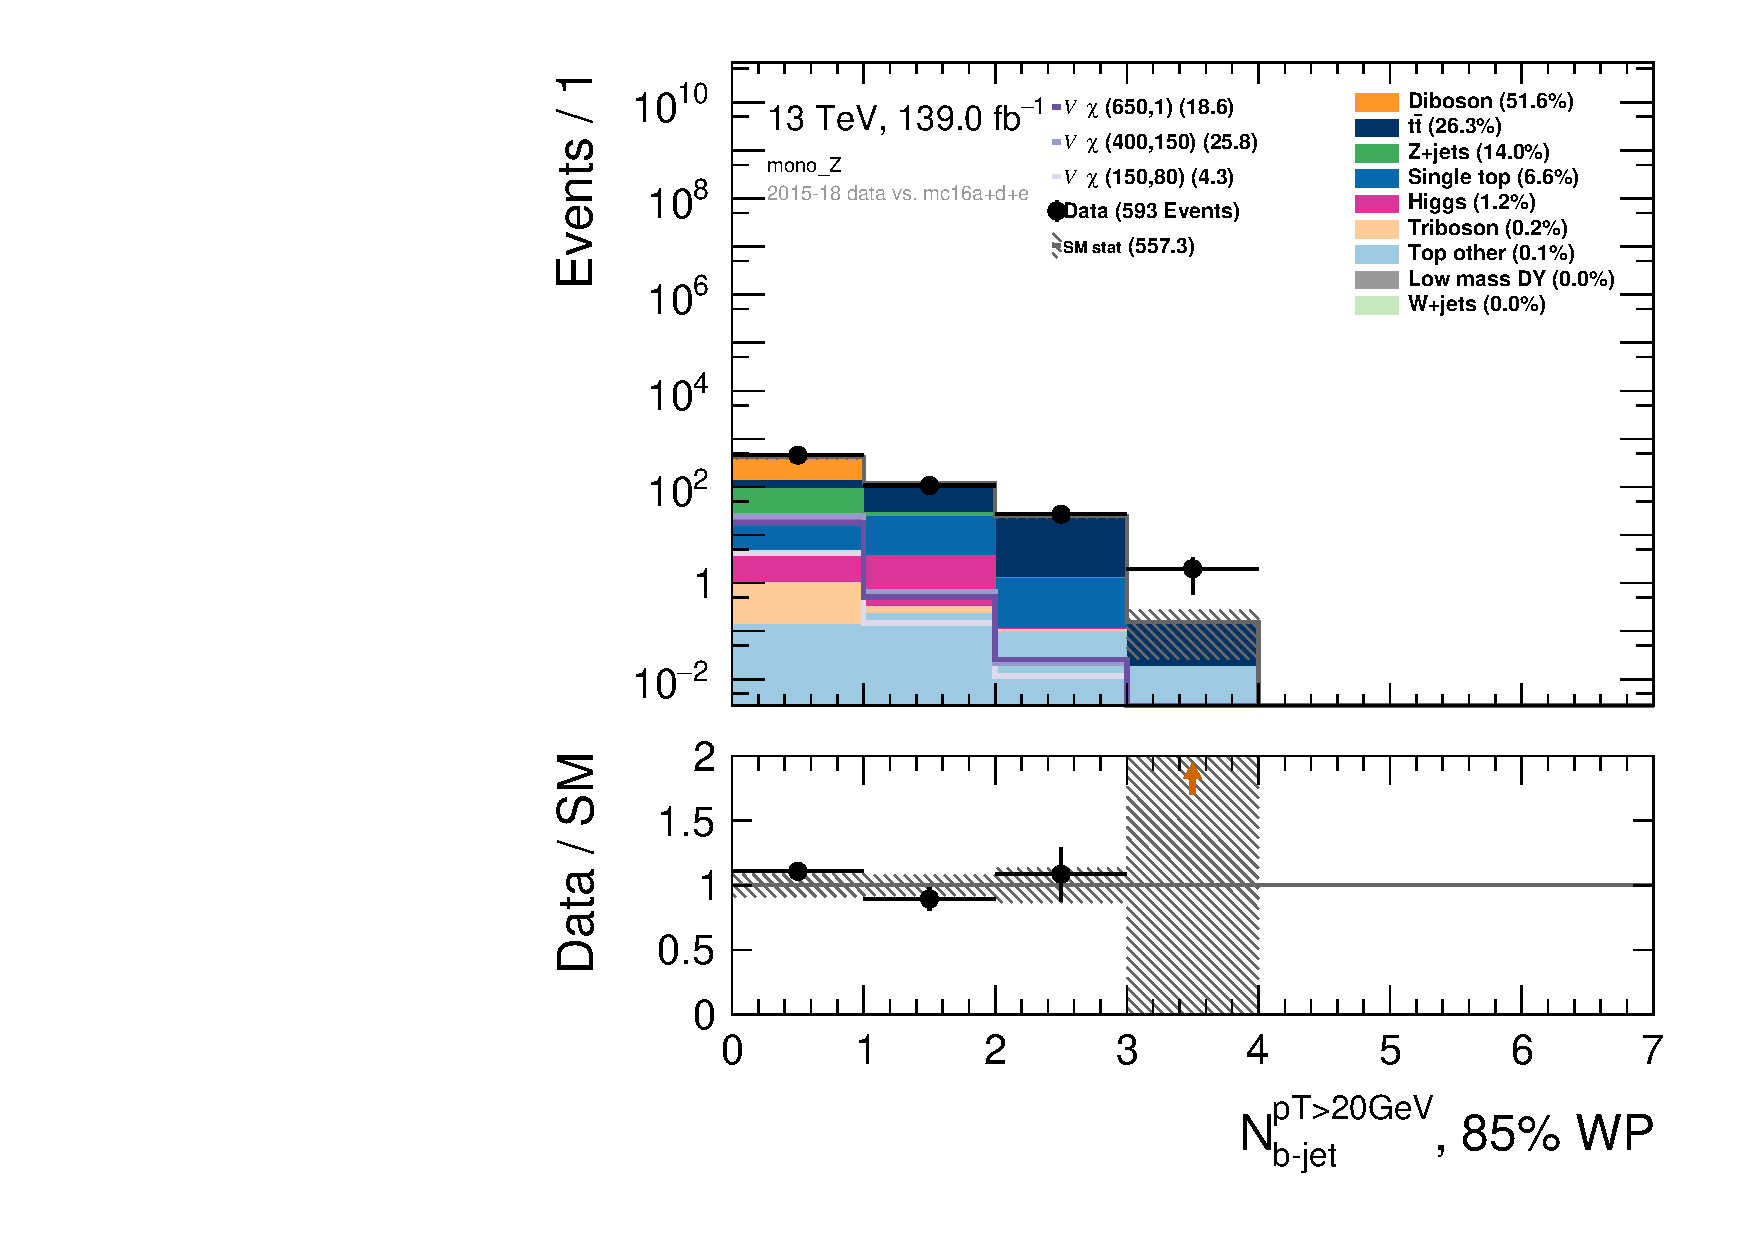
\includegraphics[width=0.5\textwidth]{Figures/MonoZcuts/hist1d_nBJet20_MV2c10_FixedCutBEff_85_mono_Z.pdf}
    \caption{Plot of the distribution of number of b-tagged jets after applying the cuts on fractional $p_T$ difference.}
    \label{fig:stepsDM4}
\end{figure}

For the signals in this case, which is maybe easier to see in table \ref{tab:cutflowDM}, we can see that it is reduced a lot. This is of course not what we want to obtain, but it is also expected after doing so many cuts as we have done. In the end of this we are going to calculate the expected significance, where we can see how much sensitivity we actually have to the signal.

\begin{landscape}
\begin{table}[H]
    \centering
    %\rotatebox{90}{
    \begin{tabular}{l l l l l l l l l}
    \toprule
    \textbf{Sample} & \textbf{2L + OS + $\mathbf{p_T}$} & $\mathbf{m_{ll}}$ & \textbf{MET} & \textbf{met/$\mathbf{H_T}$} & $\mathbf{\Delta \phi}$ & $\mathbf{\Delta R_{ll}}$ & \textbf{$\mathbf{p_T}$} \textbf{diff} & \textbf{b-jets} \\
    \midrule
    \midrule
        DY &  674647.170 & 7035.028 & 79.252 & 0.448 & 0.000 & 0.000 & 0.000 & 0.000\\
        Higgs & 1052061.840 & 1014012.858 & 3834.027 & 2116.006 & 73.416 & 46.198 & 6.942 & 3.467\\
        Single top & 189826.764 & 38267.988 & 8246.807 & 2620.670 & 73.820 & 60.859 & 36.895 & 14.845\\
        ttbar & 1854383.568 & 398898.217 & 106187.071 & 18667.204 & 439.750 & 342.455 & 146.530 & 42.570\\
        Zjets & 139141315.583 & 130368076.145 & 207856.769 & 155565.299 & 2613.607 & 1454.461 & 77.839 & 72.669\\
        Top other & 26411.801 & 6865.785 & 2104.230 & 211.226 & 3.570 & 1.880 & 0.492 & 0.136\\
        Wjets & 17813.414 & 4191.918 & 198.881 & 72.288 & 5.306 & 1.421 & 0.000 & 0.000\\
        Triboson & 528.623 & 211.477 & 81.766 & 27.851 & 1.406 & 1.332 & 0.999 & 0.900\\
        Diboson & 467672.290 & 270103.987 & 15853.093 & 7702.570 & 394.866 & 367.781 & 287.632 & 278.123\\
        Data & 146385200.000 & 134795284.000 & 337736.000 & 175111.000 & 3287.000 & 2116.000 & 593.000 & 457.000\\
        $( V, \chi) (150, 80)$ & 196.844 & 188.682 & 105.505 & 83.150 & 4.866 & 4.765 & 4.325 & 4.166\\
        $( V, \chi) (400, 150)$ & 945.406 & 904.916 & 573.904 & 459.476 & 28.740 & 28.194 & 25.789 & 25.124\\
        $( V, \chi) (650, 1)$  & 633.417 & 605.474 & 425.291 & 343.235 & 20.533 & 20.193 & 18.566 & 18.019\\
        \bottomrule
    \end{tabular}
    %}
    \caption{A cut flow overview after applying the different cuts in table \ref{tab:cutsDM}.}
    \label{tab:cutflowDM}
\end{table}
\end{landscape}





\begin{comment}


\newgeometry{twoside,inner=3cm,outer=2cm}
\begin{figure}[H]
%\begin{minipage}{2\textwidth}
%\begin{adjustwidth}{-3cm}{-3cm}
\centering
%\advance\leftskip-4cm 
%\advance\rightskip-4cm 
    \begin{subfigure}[t!]{0.49\textwidth}
        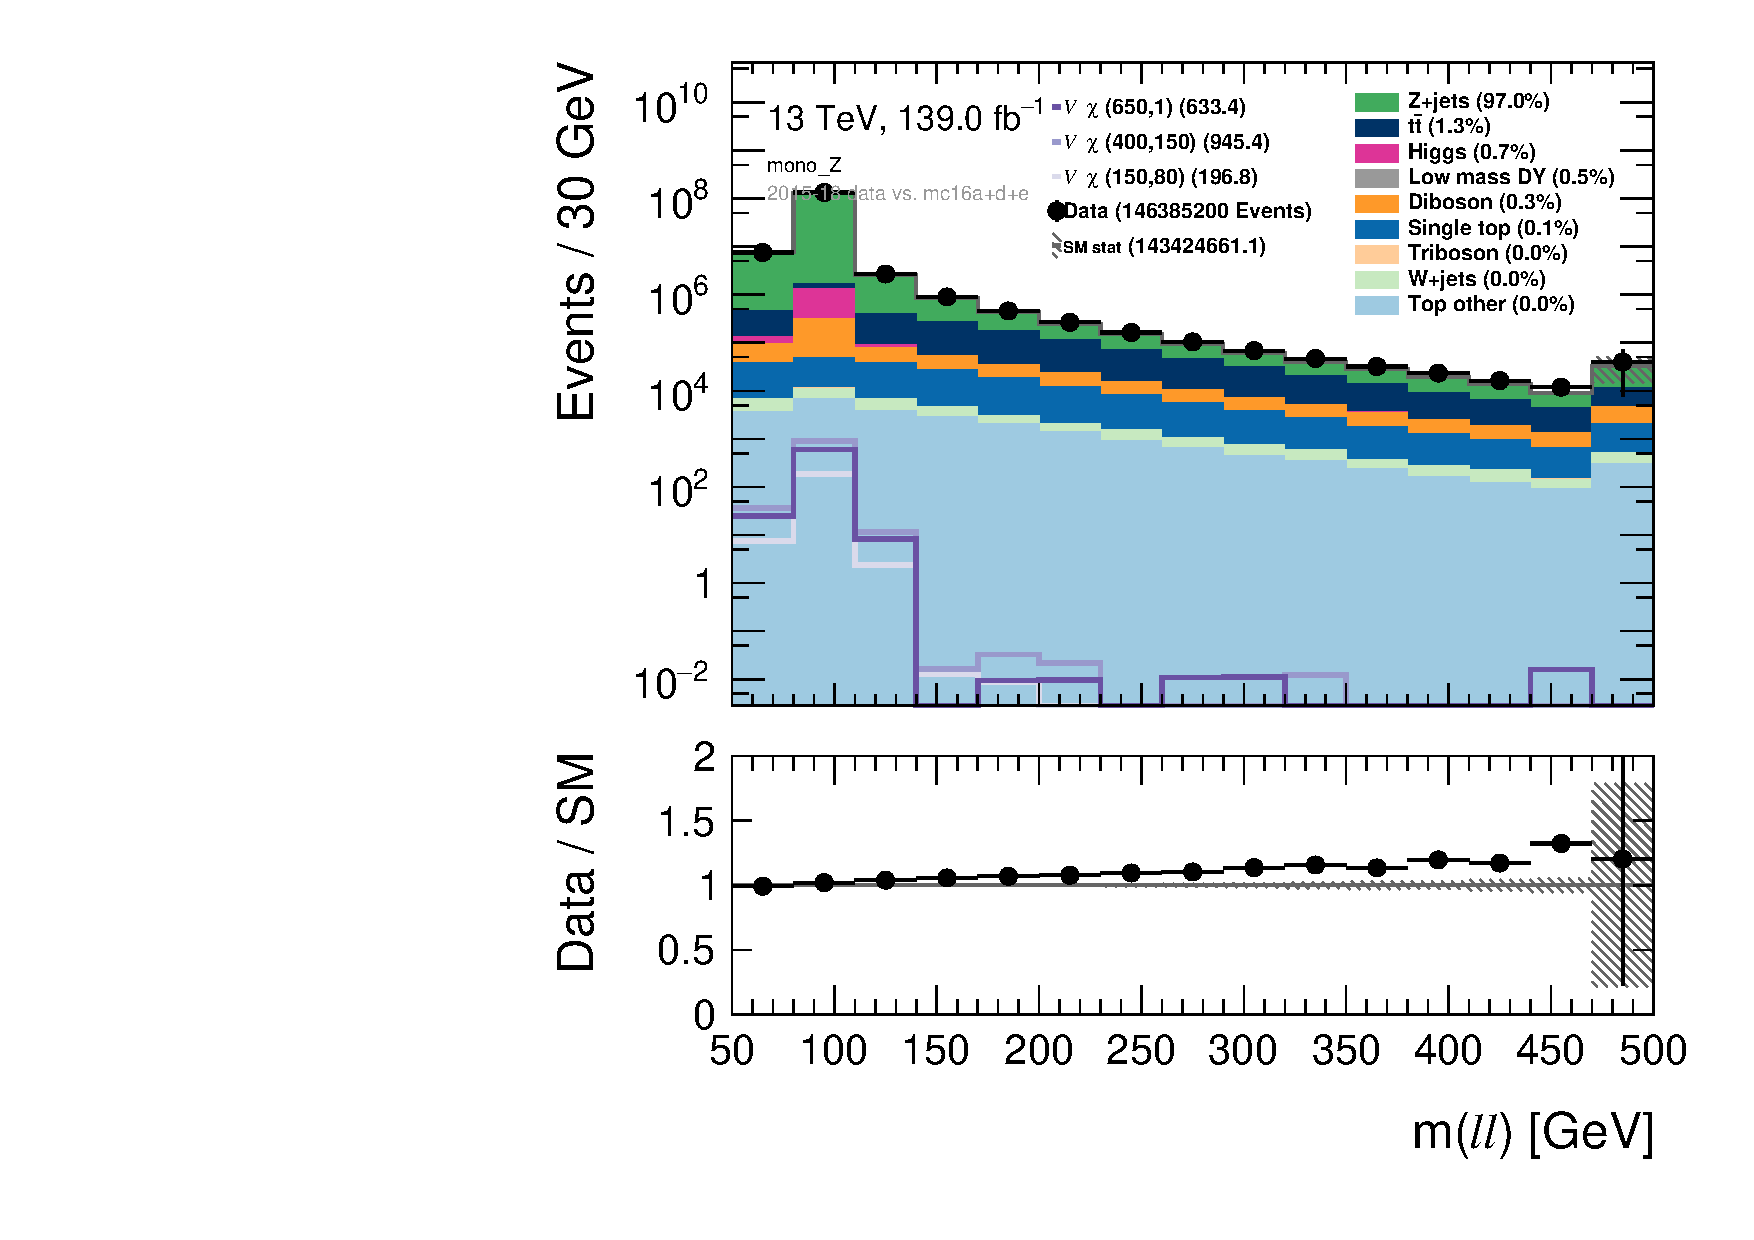
\includegraphics[width=\textwidth]{Figures/MonoZcuts/hist1d_mll_mono_Z.pdf}
    \caption{Stransverse mass for direct slepton production.}
    \label{fig:my_label}
    \end{subfigure}
    \begin{subfigure}[t!]{0.49\textwidth}
        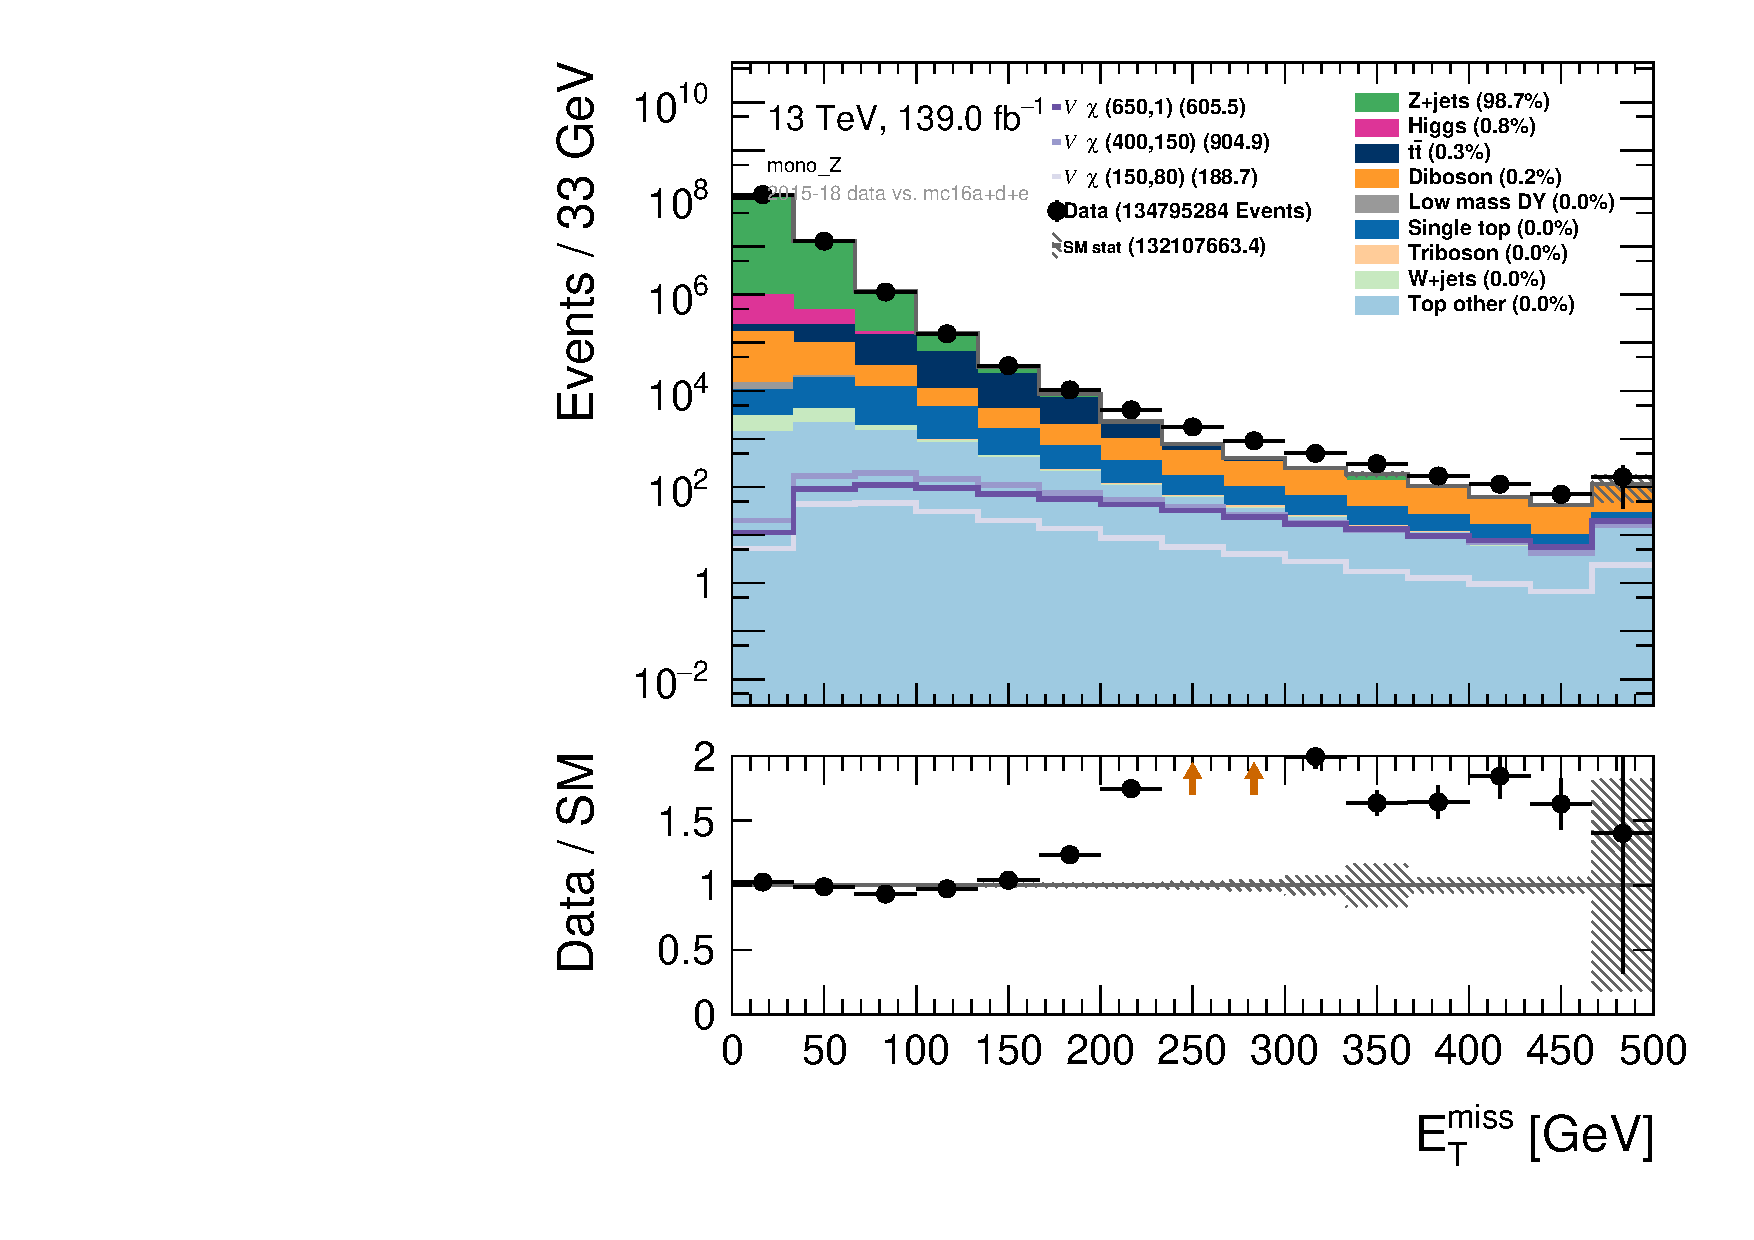
\includegraphics[width=\textwidth]{Figures/MonoZcuts/hist1d_met_Et_mono_Z_1.pdf}
    \caption{Stransverse mass for chargino production via $\Tilde{l}/\Tilde{\nu}$.}
    \label{fig:my_label}
    \end{subfigure}
    \\
    \begin{subfigure}[t!]{0.49\textwidth}
        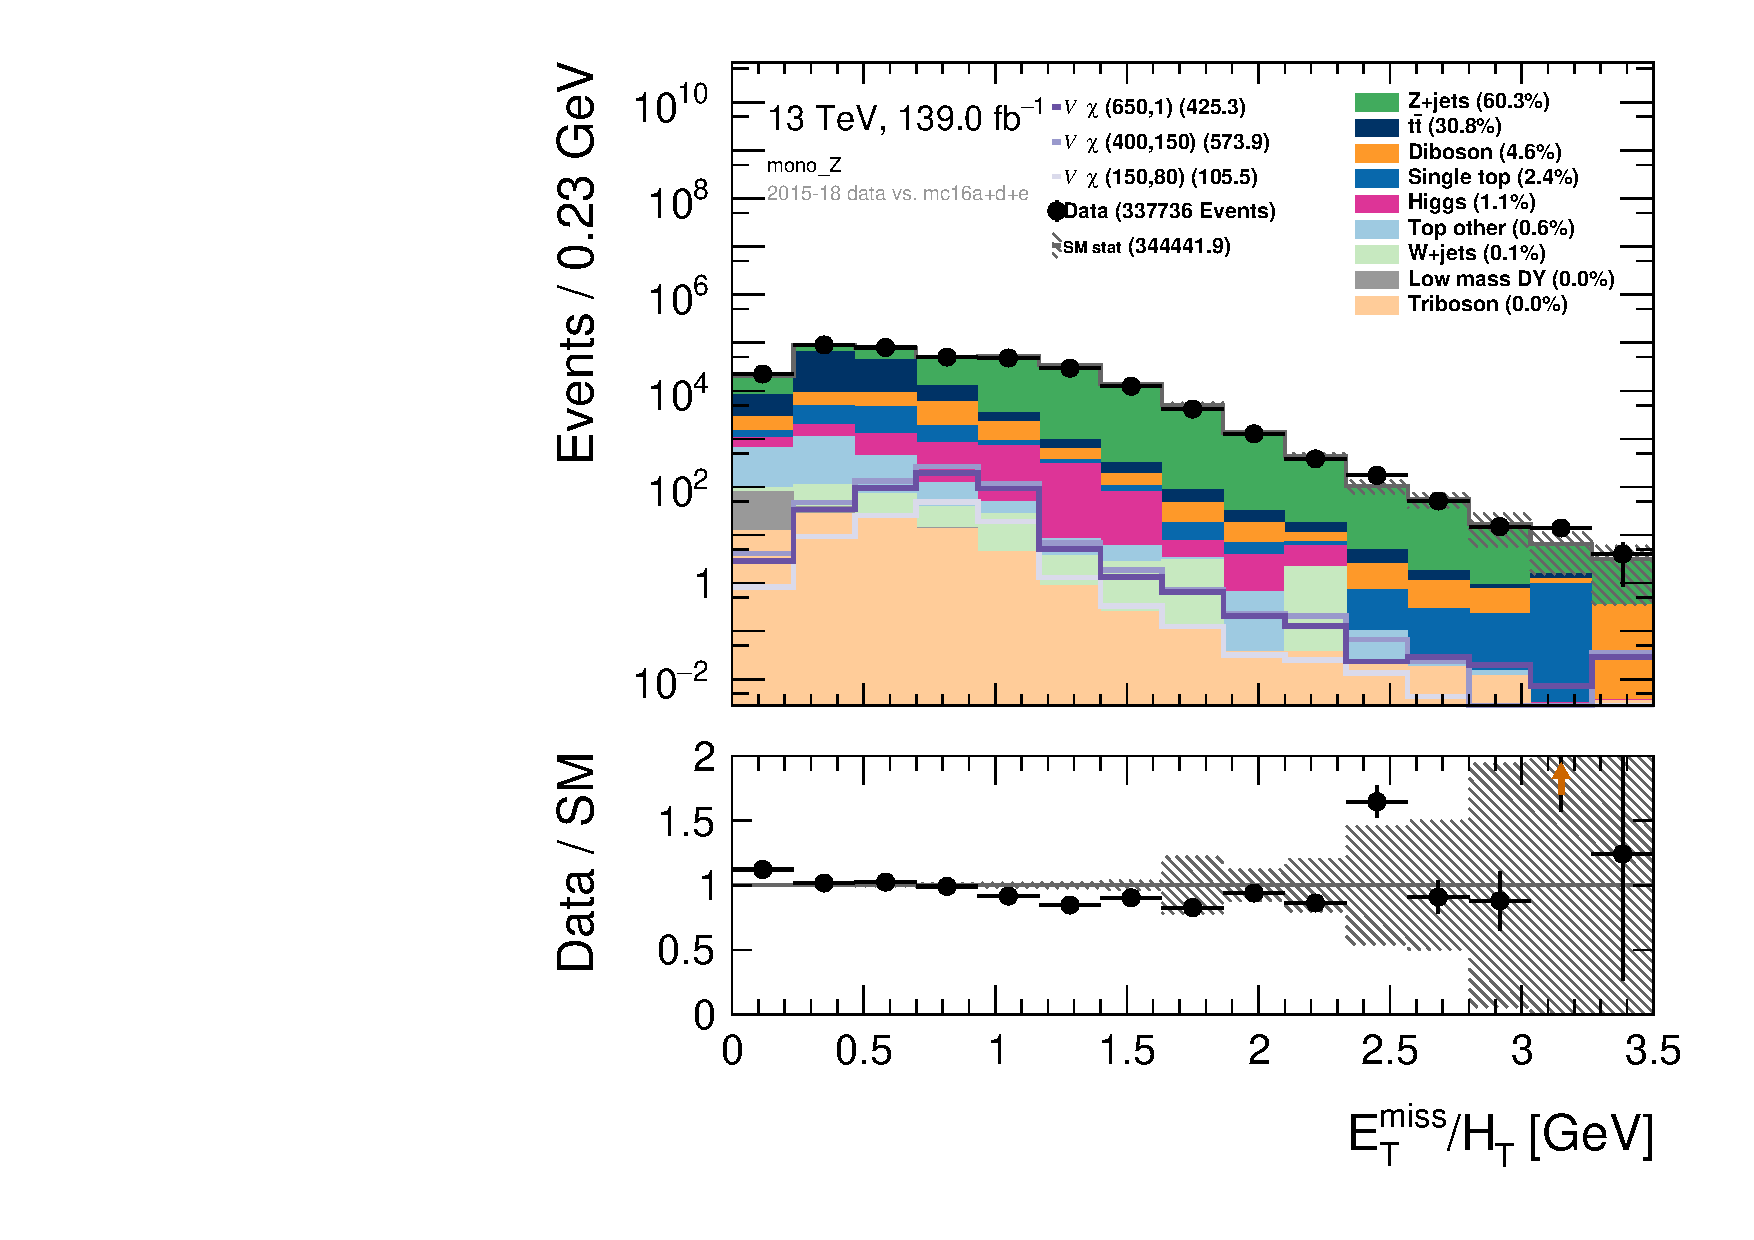
\includegraphics[width=\textwidth]{Figures/MonoZcuts/hist1d_met_HT_mono_Z.pdf}
    \caption{Stransverse mass for chargino production via $W^\pm$.}
    \label{fig:my_label}
    \end{subfigure}
    \begin{subfigure}[t!]{0.49\textwidth}
        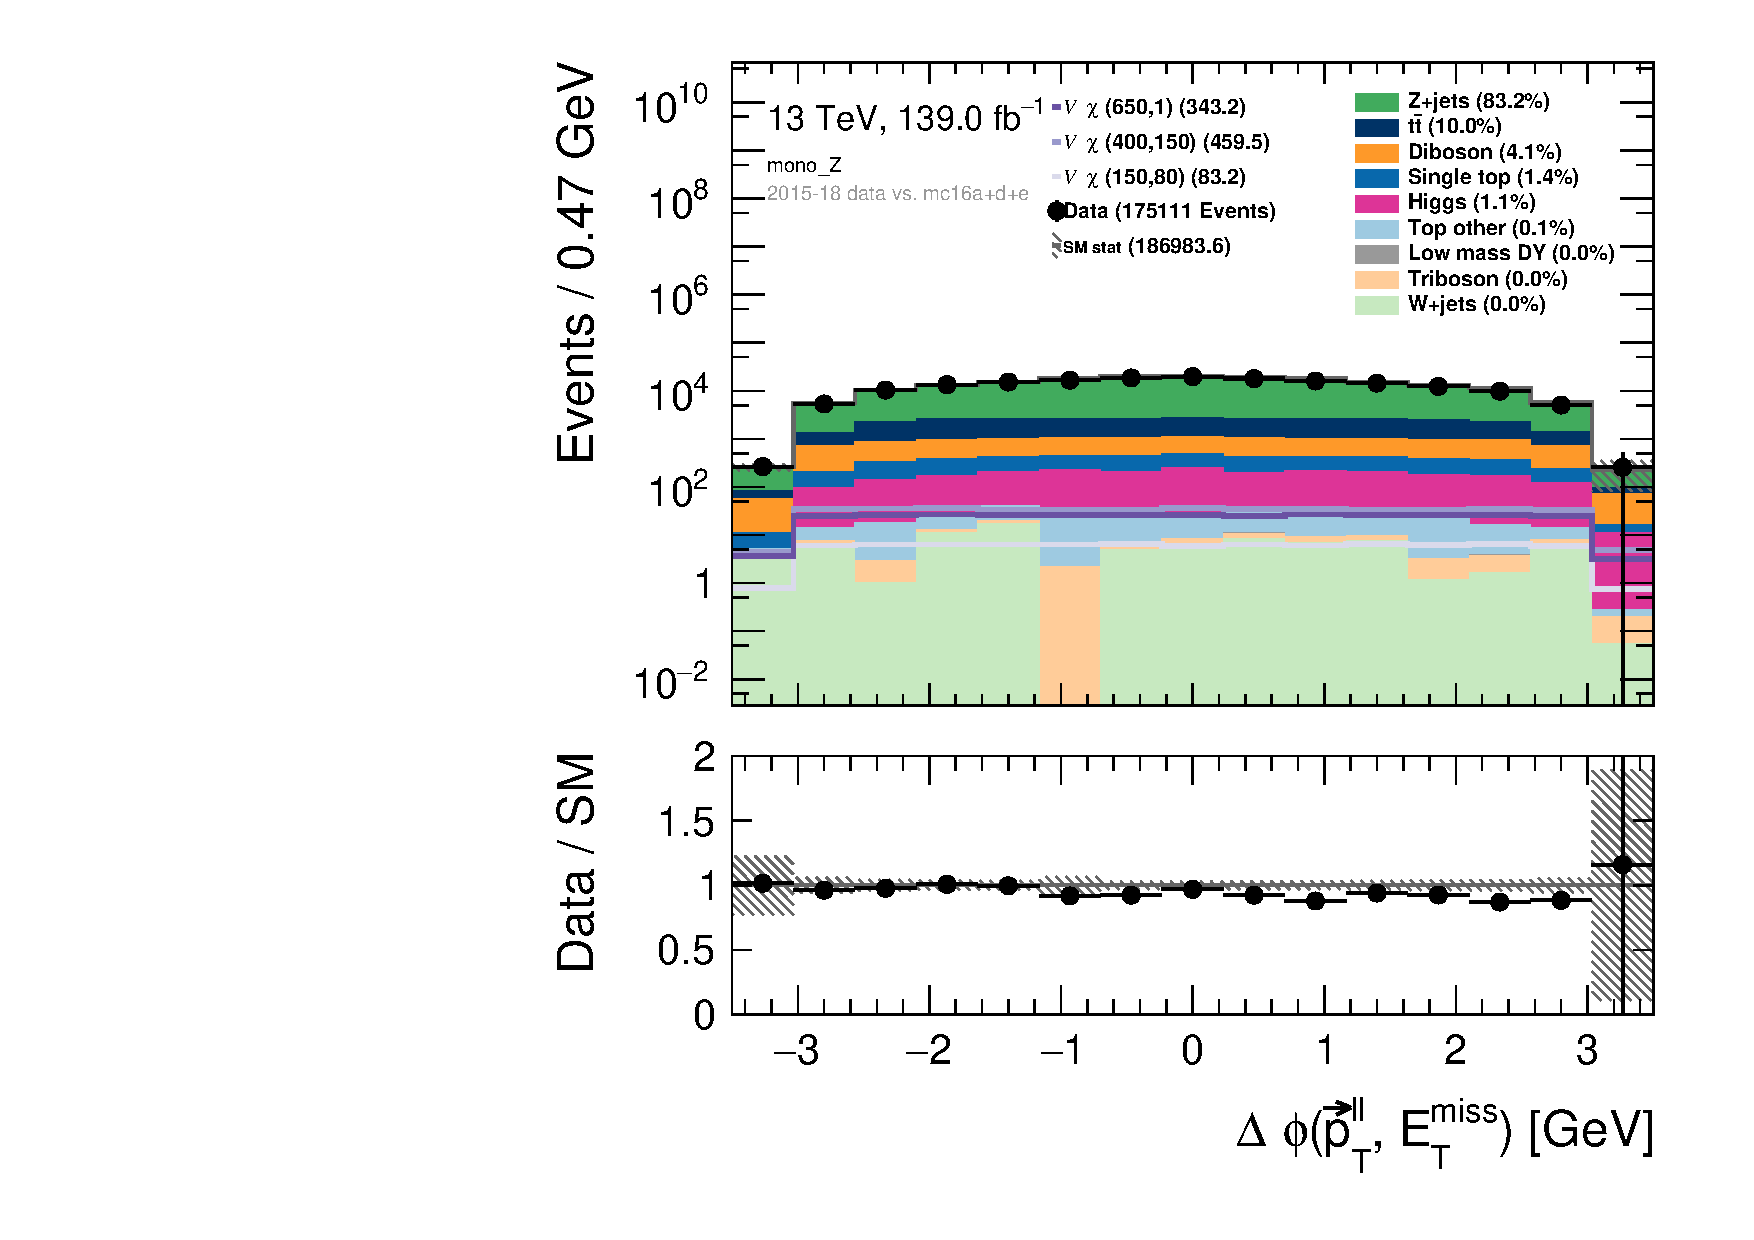
\includegraphics[width=\textwidth]{Figures/MonoZcuts/hist1d_deltaPhi_mono_Z.pdf}
    \caption{Missing transverse energy for mono-Z.}
    \label{fig:my_label}
    \end{subfigure}
    \\
    \begin{subfigure}[t!]{0.49\textwidth}
        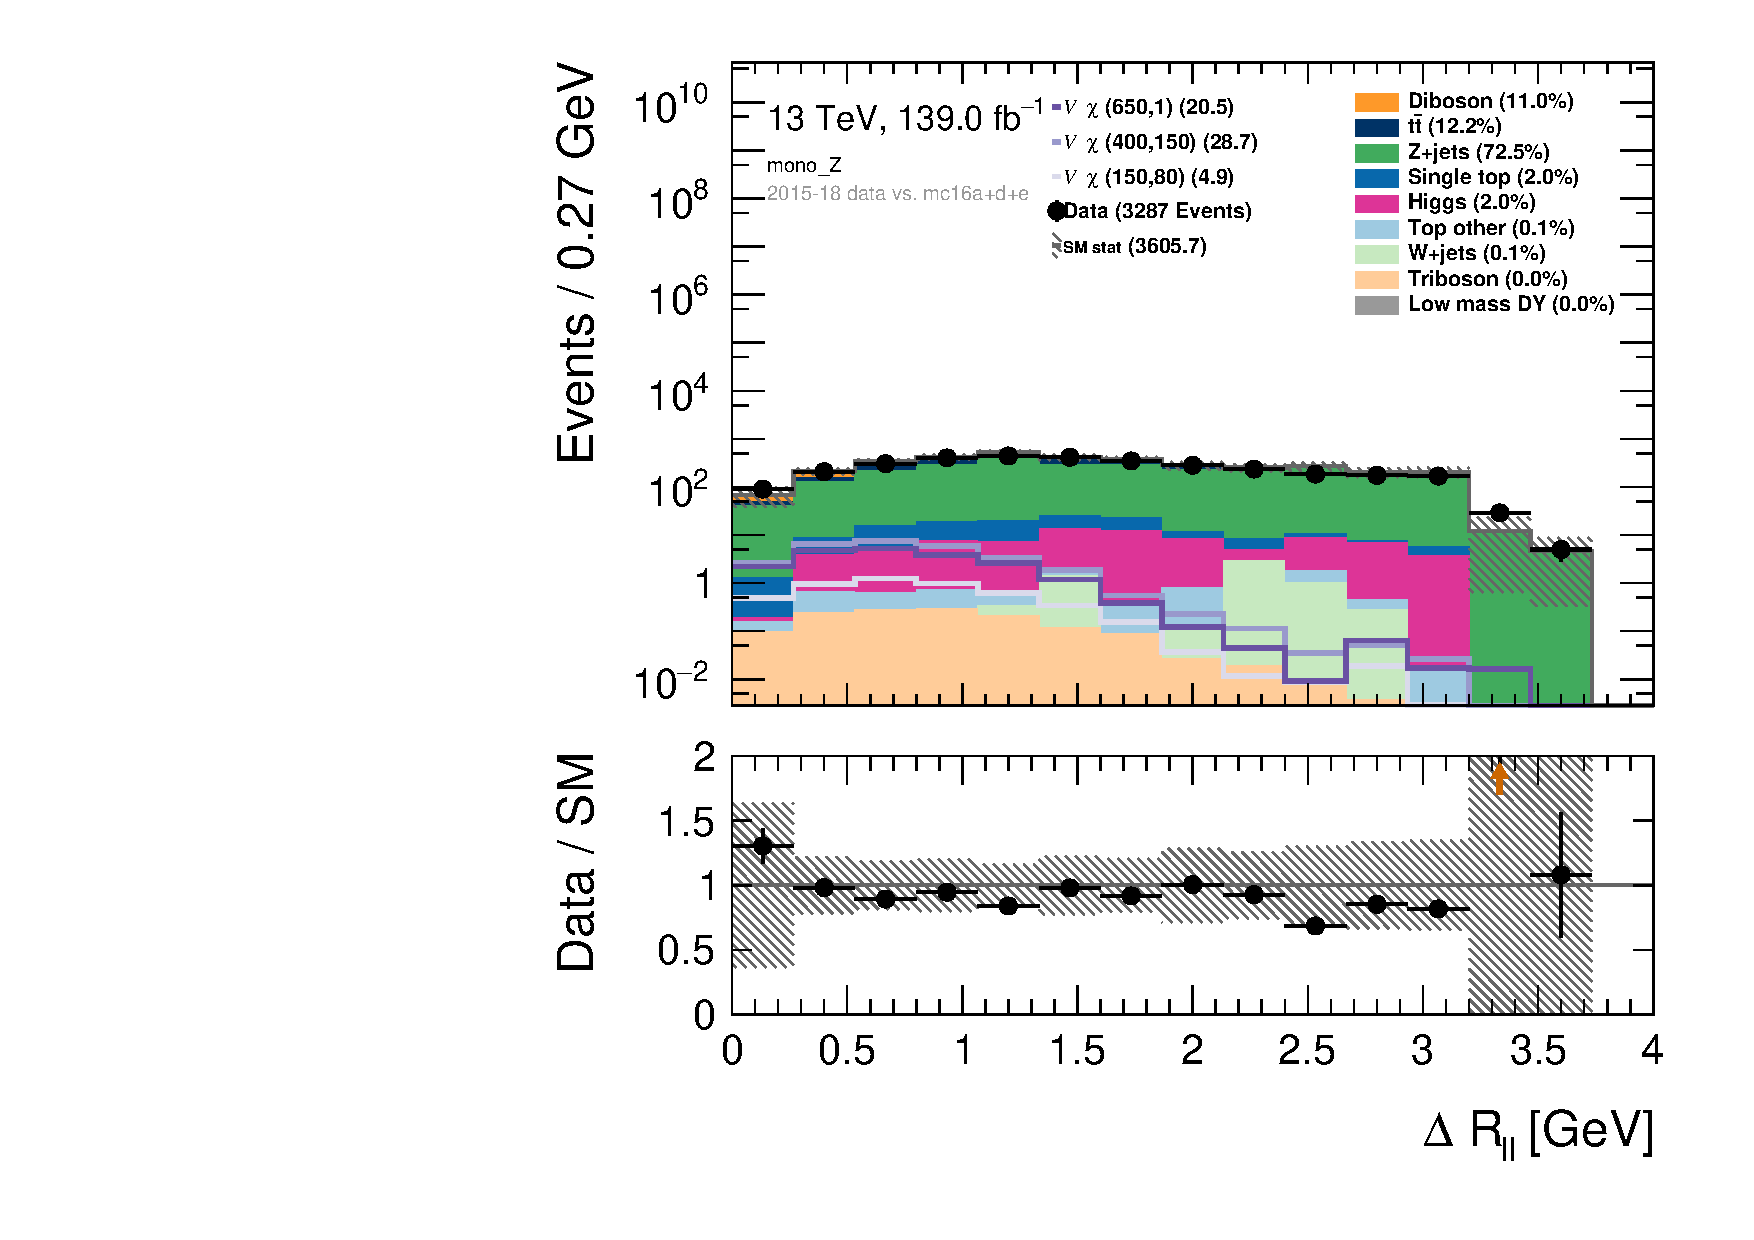
\includegraphics[width=\textwidth]{Figures/MonoZcuts/hist1d_deltaRll_mono_Z.pdf}
    \caption{Stransverse mass for chargino production via $W^\pm$.}
    \label{fig:my_label}
    \end{subfigure}
    \begin{subfigure}[t!]{0.49\textwidth}
        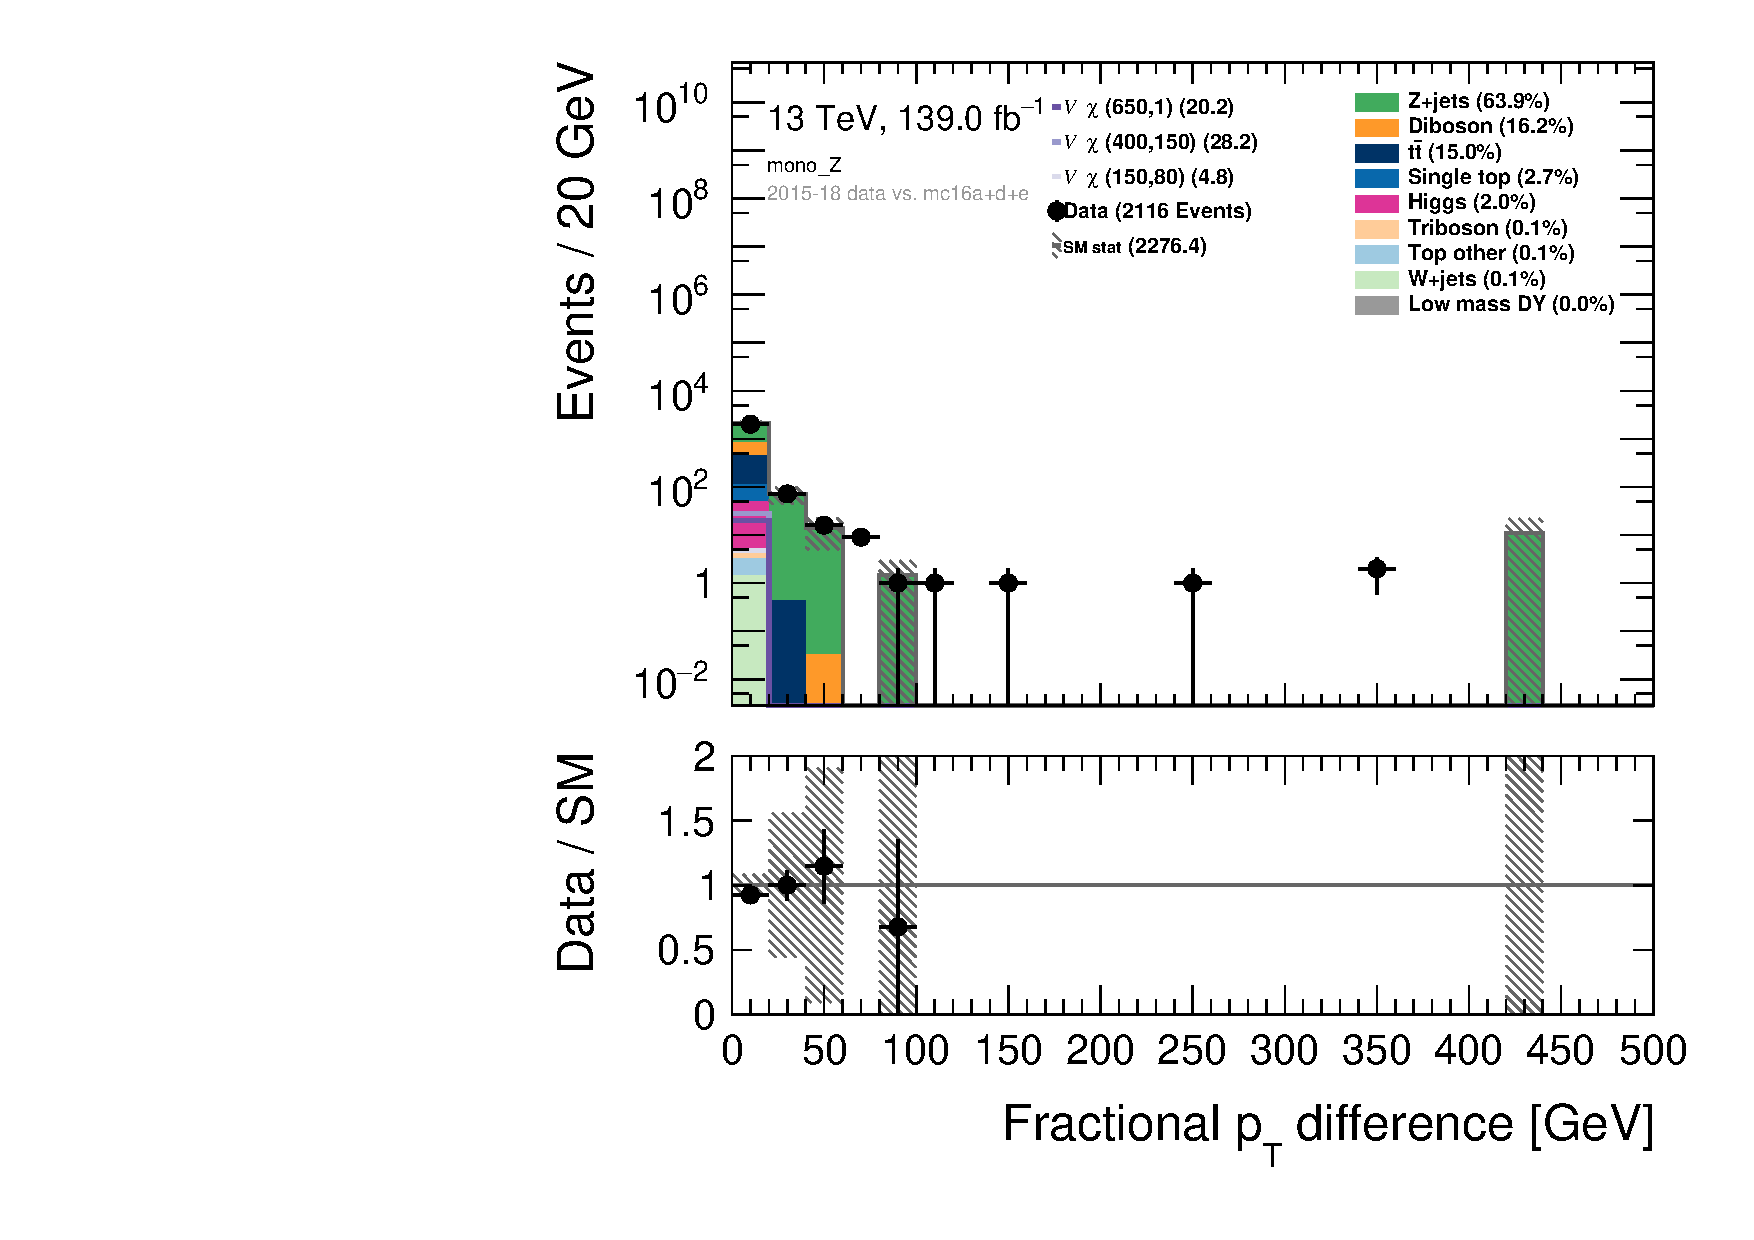
\includegraphics[width=\textwidth]{Figures/MonoZcuts/hist1d_pTdiff_mono_Z.pdf}
    \caption{Missing transverse energy for mono-Z.}
    \label{fig:my_label}
    \end{subfigure}
\end{figure}
\restoregeometry


\newgeometry{twoside,inner=3cm,outer=2cm}
\begin{figure}[H] \ContinuedFloat
%\begin{minipage}{2\textwidth}
%\begin{adjustwidth}{-3cm}{-3cm}
\centering
%\advance\leftskip-4cm 
%\advance\rightskip-4cm 
    \begin{subfigure}[t!]{0.49\textwidth}
        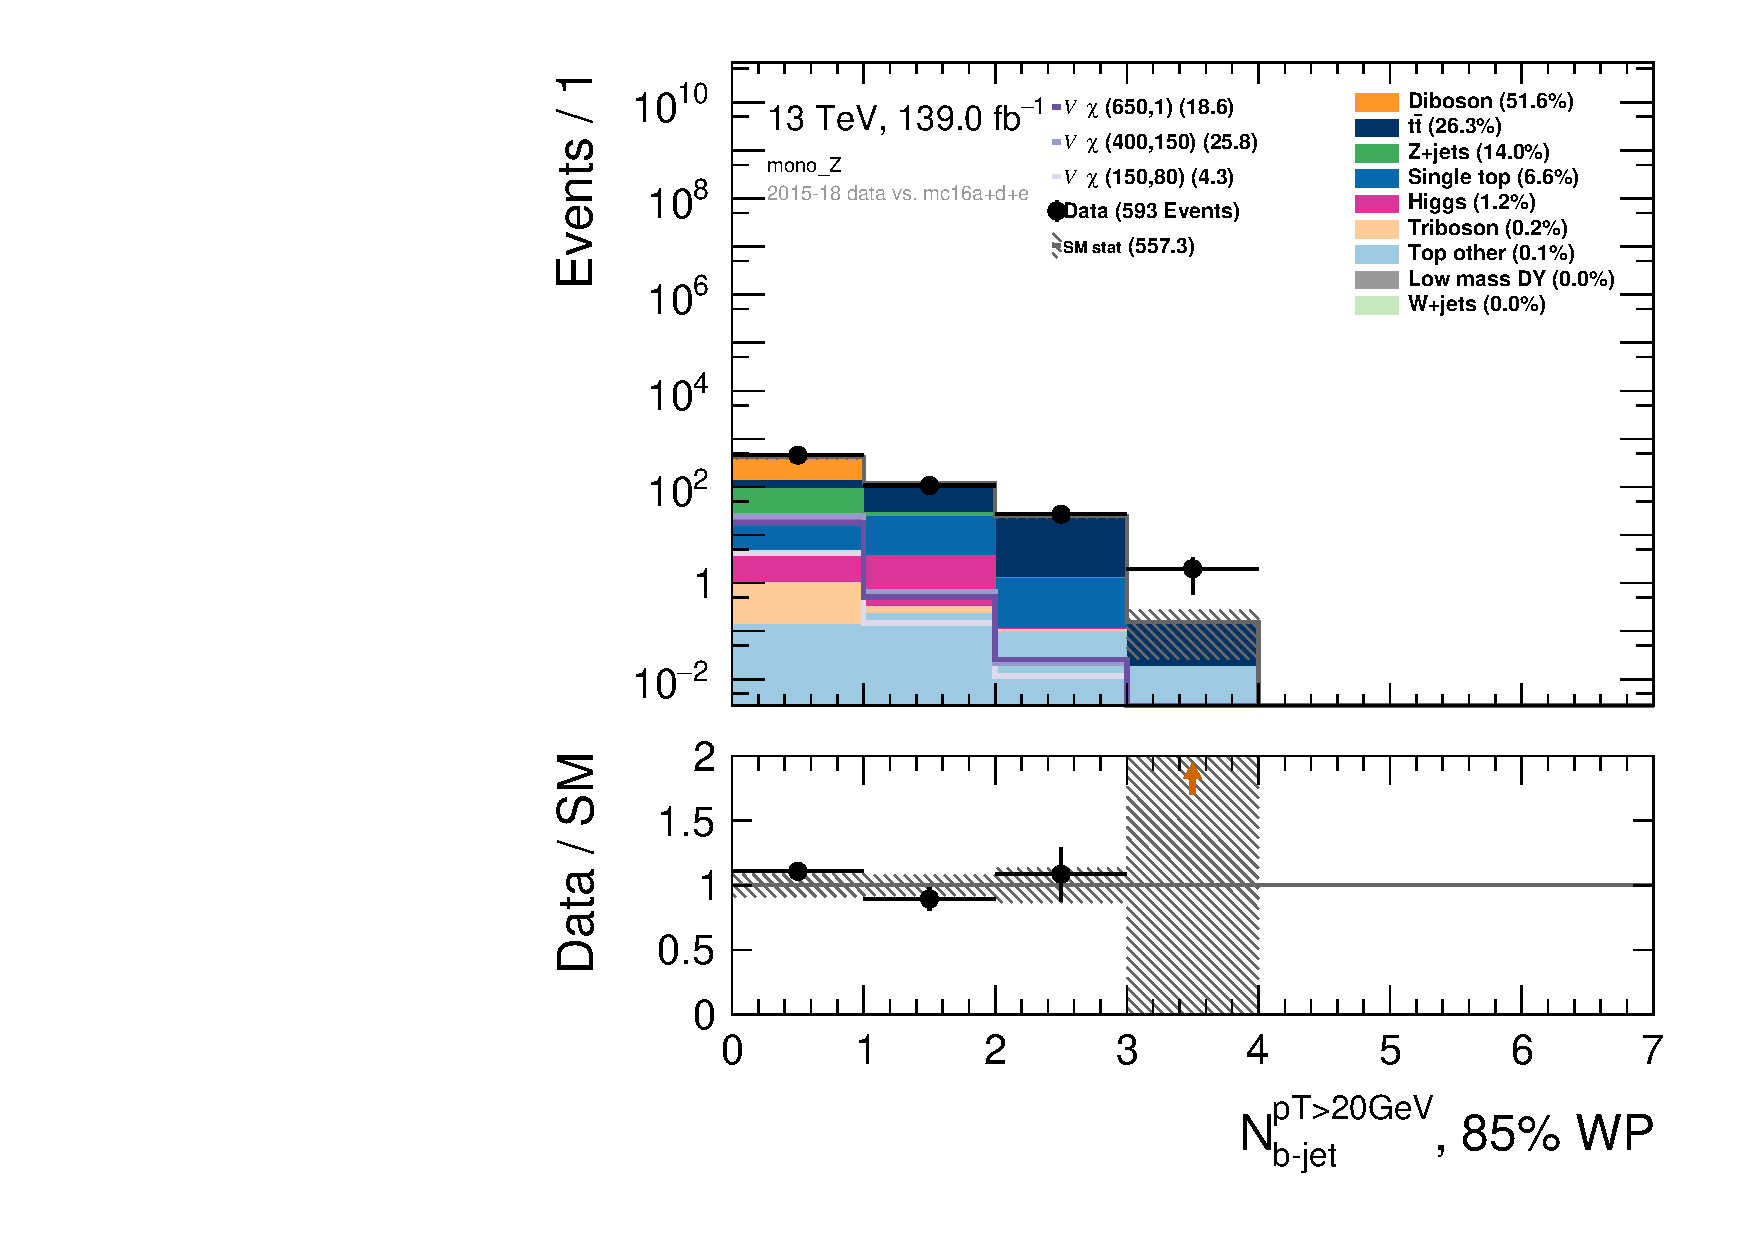
\includegraphics[width=\textwidth]{Figures/MonoZcuts/hist1d_nBJet20_MV2c10_FixedCutBEff_85_mono_Z.pdf}
    \caption{Stransverse mass for direct slepton production.}
    \label{fig:my_label}
    \end{subfigure}
    \begin{subfigure}[t!]{0.49\textwidth}
        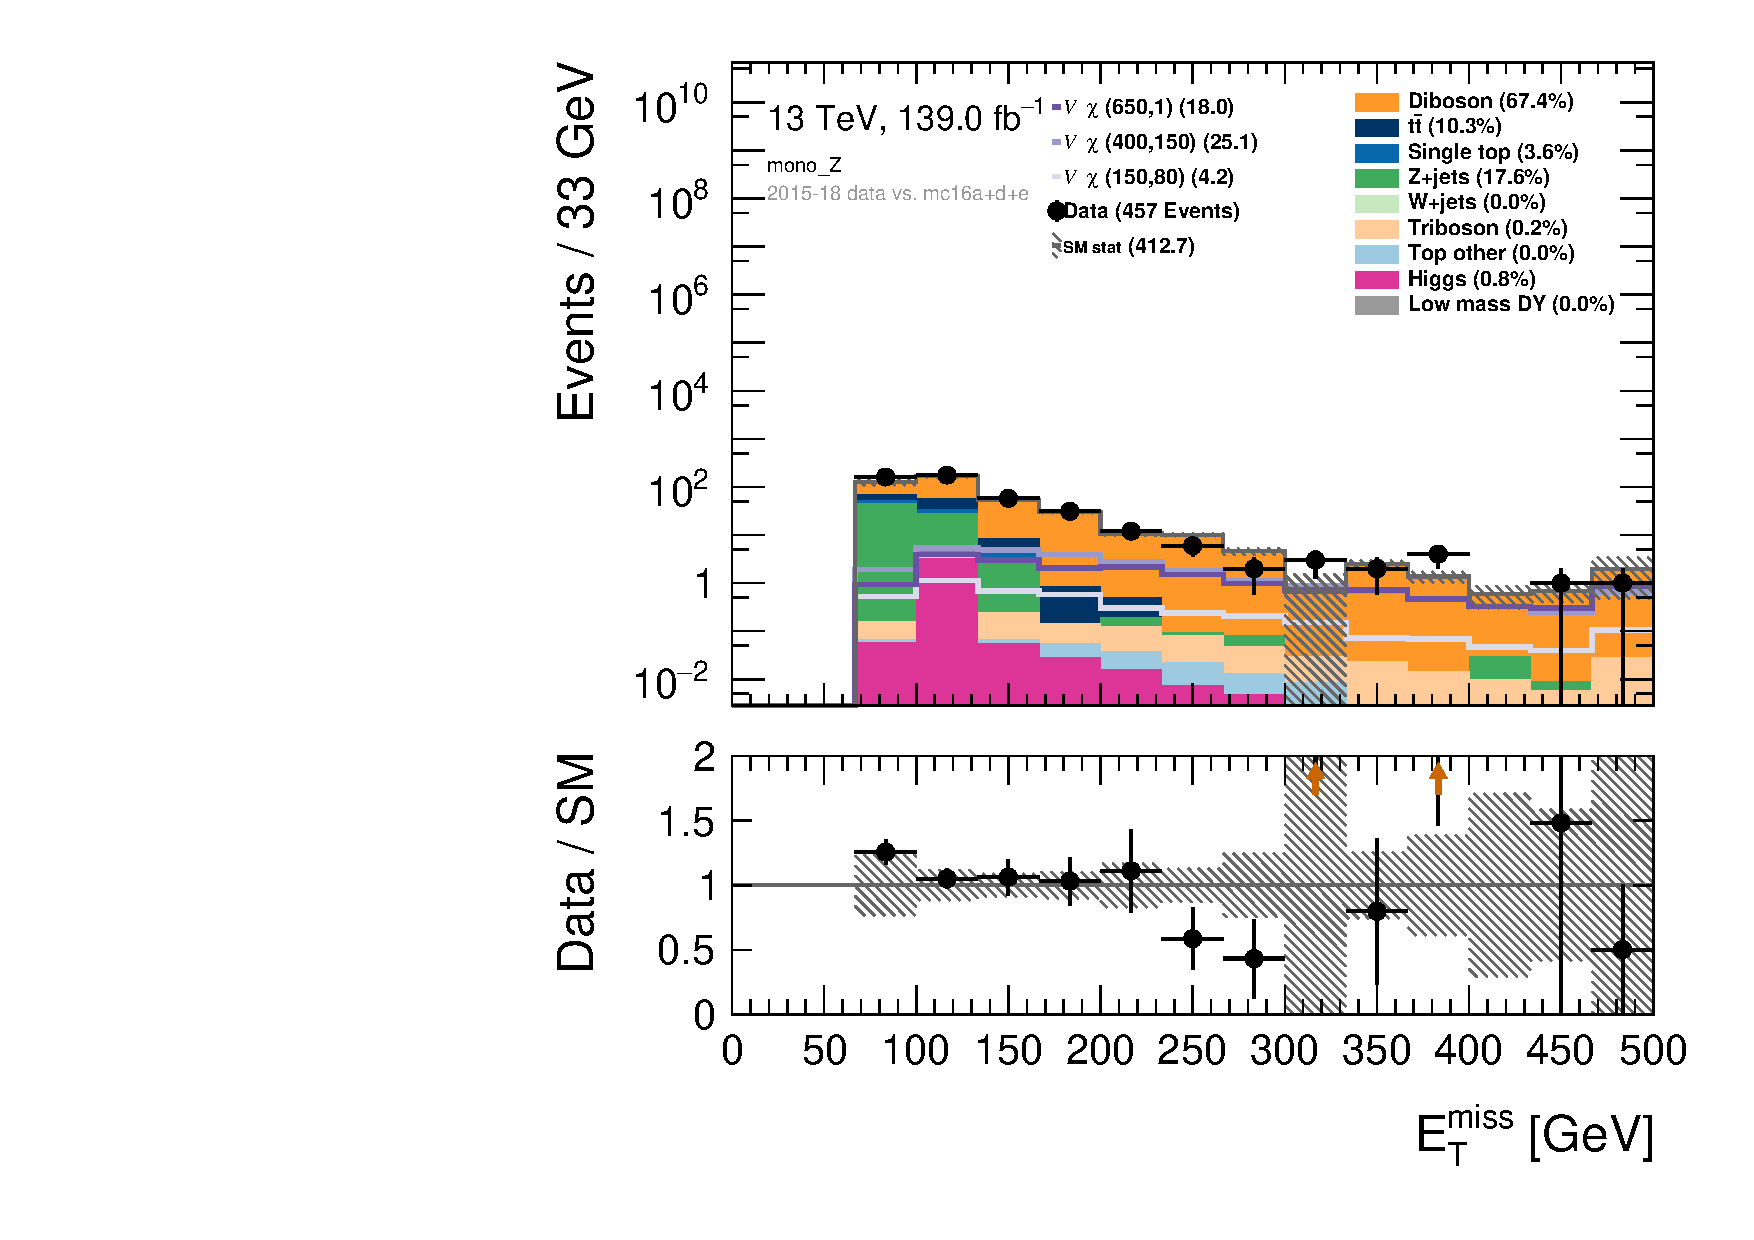
\includegraphics[width=\textwidth]{Figures/MonoZcuts/hist1d_met_Et_mono_Z.pdf}
    \caption{Stransverse mass for chargino production via $\Tilde{l}/\Tilde{\nu}$.}
    \label{fig:my_label}
    \end{subfigure}
    \caption{Plot of the four most important variables in direct slepton production with a cut on only two leptons with opposite charge in the final state.}
    \label{fig:cutandcountStepsDM}
\end{figure}
\restoregeometry
\end{comment}


All of the cuts are applied to get fewer background events while we, at the same time, do not want to cut away too much of the signal events. The publications have applied more or less the same cuts as listed above in table \ref{tab:cutsSUSY} and \ref{tab:cutsDM}, and their results are presented in figure \ref{fig:atlaspub}.


\begin{figure}[H]
\centering
    \begin{subfigure}[H]{0.49\textwidth}
        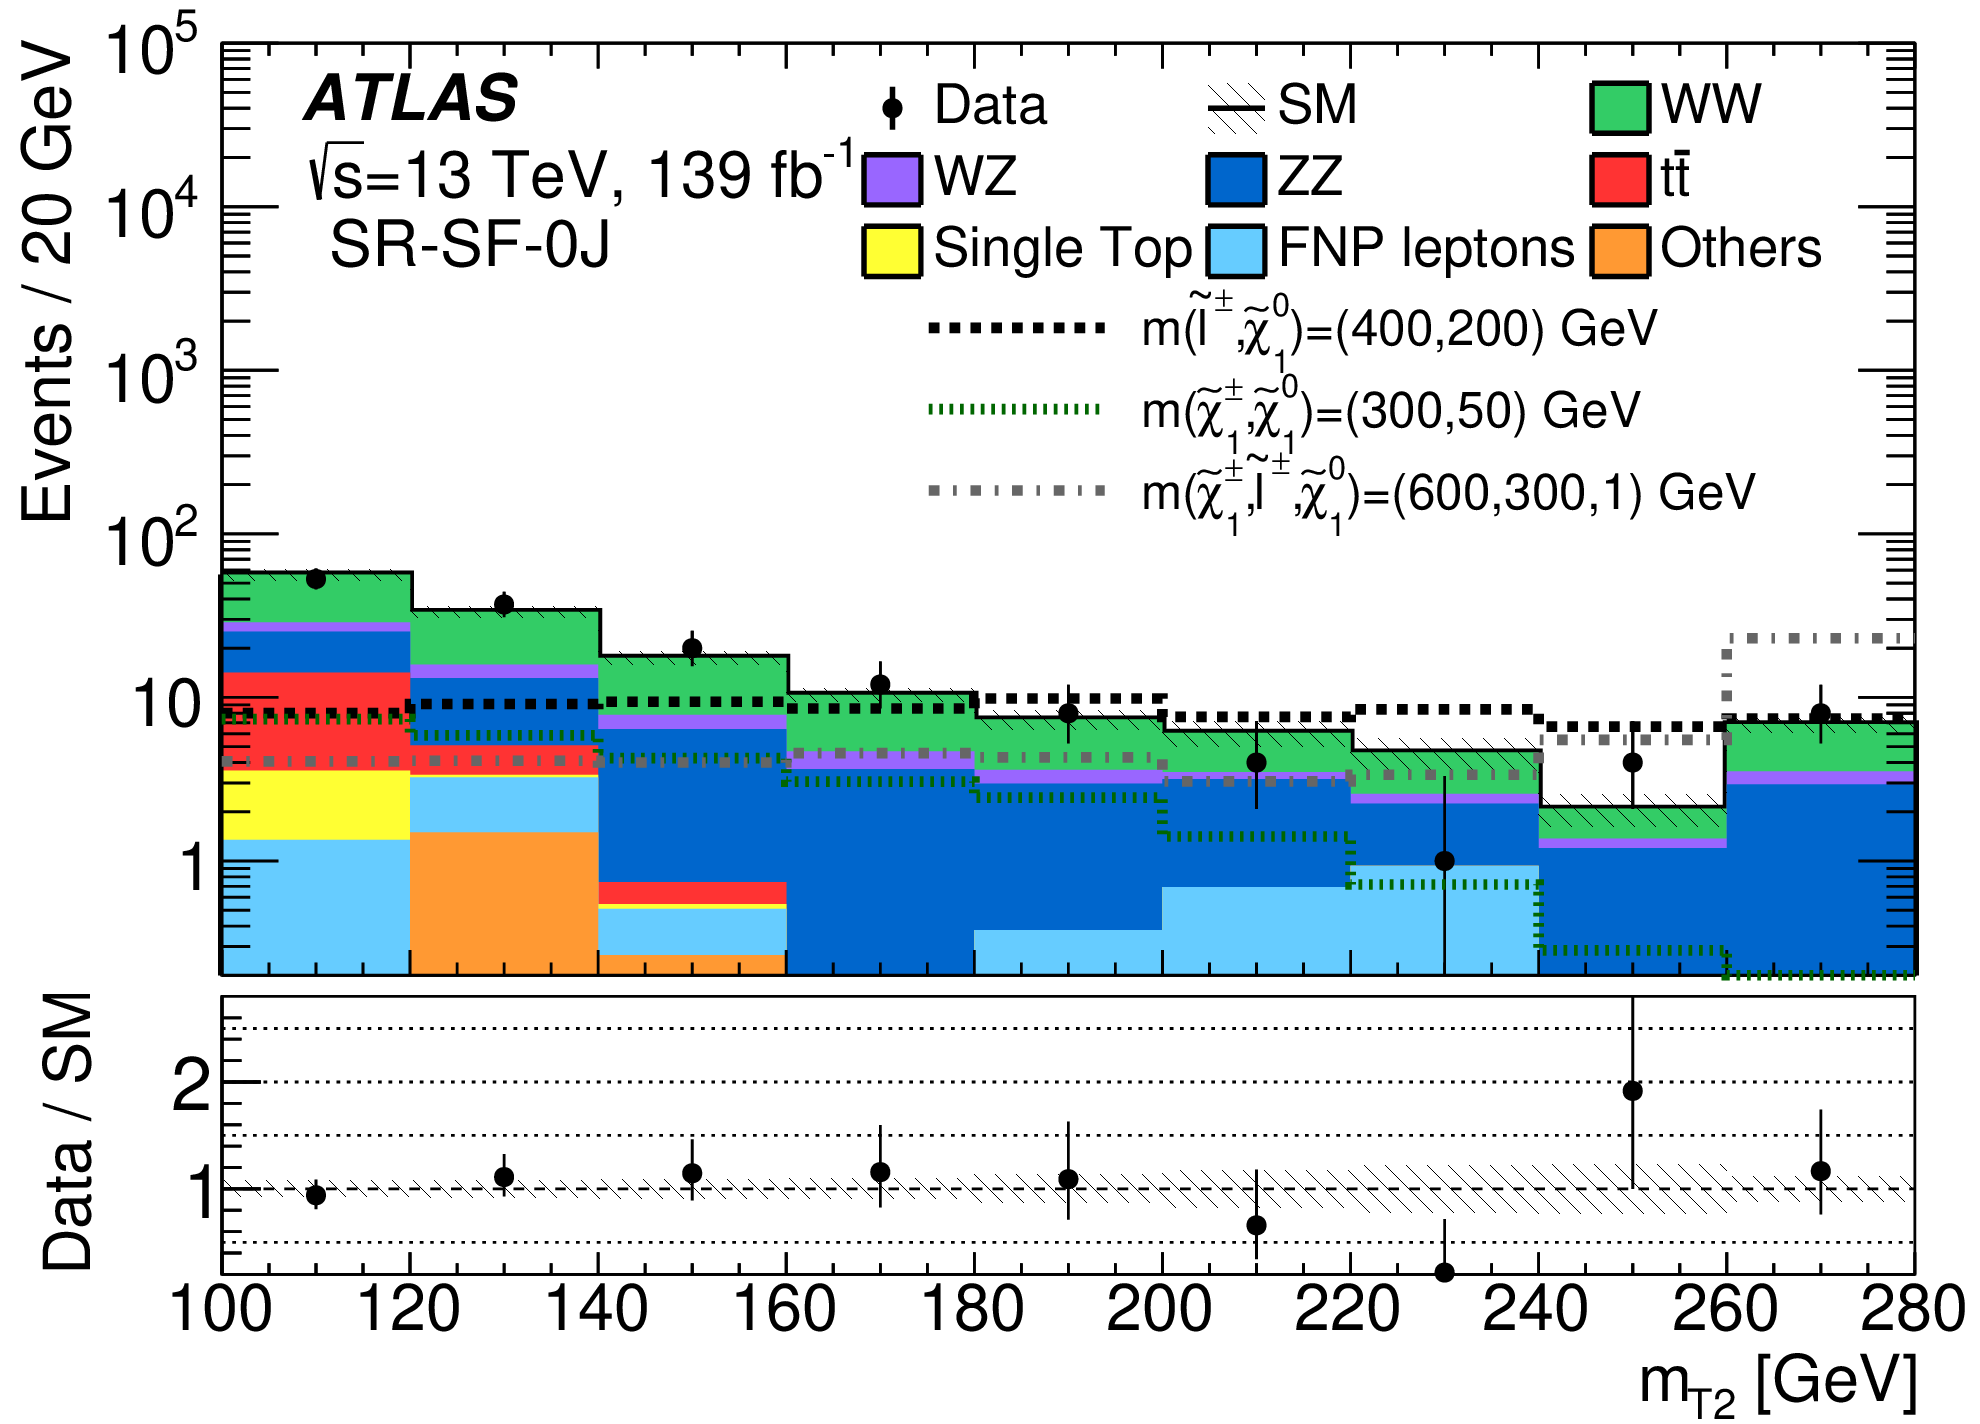
\includegraphics[width=\textwidth]{Figures/FromOnline/atlasmt2SUSY.png}
    \caption{Stransverse mass for direct slepton production, chargino production with $\Tilde{l}/\Tilde{\nu}$-mediated decays and with W-boson-mediated decays.}
    \label{fig:atlasSUSY}
    \end{subfigure}
    \\
    \begin{subfigure}[H]{\textwidth}
        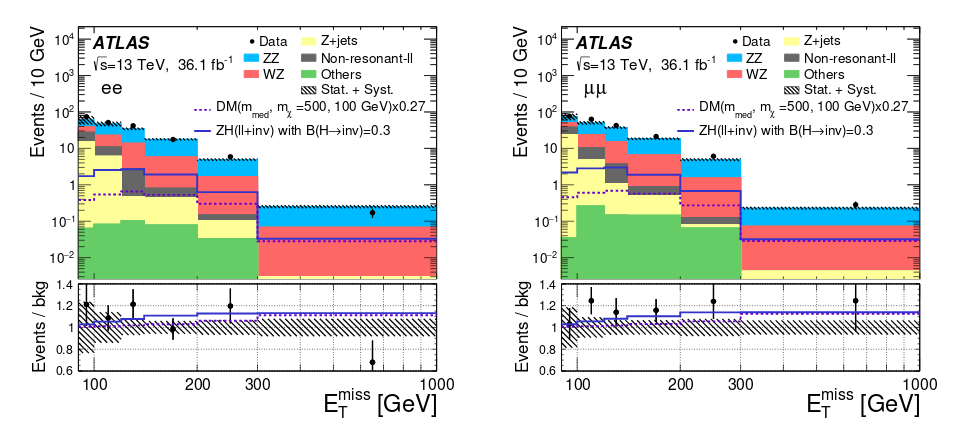
\includegraphics[width=\textwidth]{Figures/FromOnline/atlasmetDM.png}
    \caption{Missing transverse energy for the mono-Z process, where the left plot is the electron channel and right is the muon channel.}
    \label{fig:atlasDM}
    \end{subfigure}
    \caption{Results from the ATLAS publications for the four processes considered in this thesis.}
    \label{fig:atlaspub}
\end{figure}


In figure \ref{fig:atlasSUSY}, we can see that the signal is separated from the background for both the direct slepton production and the chargino production with W-boson-mediated-decay. However, they have not obtained any significant separation for chargino production with slepton/sneutrino-mediated-decay, which means that we should not expect to claim any discovery for the signal model shown in these plots. 

In figure \ref{fig:atlasDM}, we can see the plots for both electron channel and muon channel for the mono-Z process. It is not as much separation between signal and background as for the direct slepton production and the chargino production with W-boson-mediated-decay, but there is some. 

Later in this thesis, we will calculate the expected significance for the different processes we are looking at with both cut and count and ML. This is not done in the publications we are looking at, but they have included an exclusion plot which we can use for comparison later. This is shown in figure \ref{fig:exclusionPlots}. Here we can see the expected exclusion limit with $\pm1\sigma$ uncertainty bin together with the observed exclusion limit. The expected exclusion curve in these plots follow the boundary where the significance is 1.36 (i.e. 95\% CL exclusion). We are not going to reproduce these results in this thesis. However, we have used it to pick out some benchmark signals around the expected exclusion limit. 

\begin{figure}[H]
    \centering
    \begin{subfigure}[t!]{0.49\textwidth}
        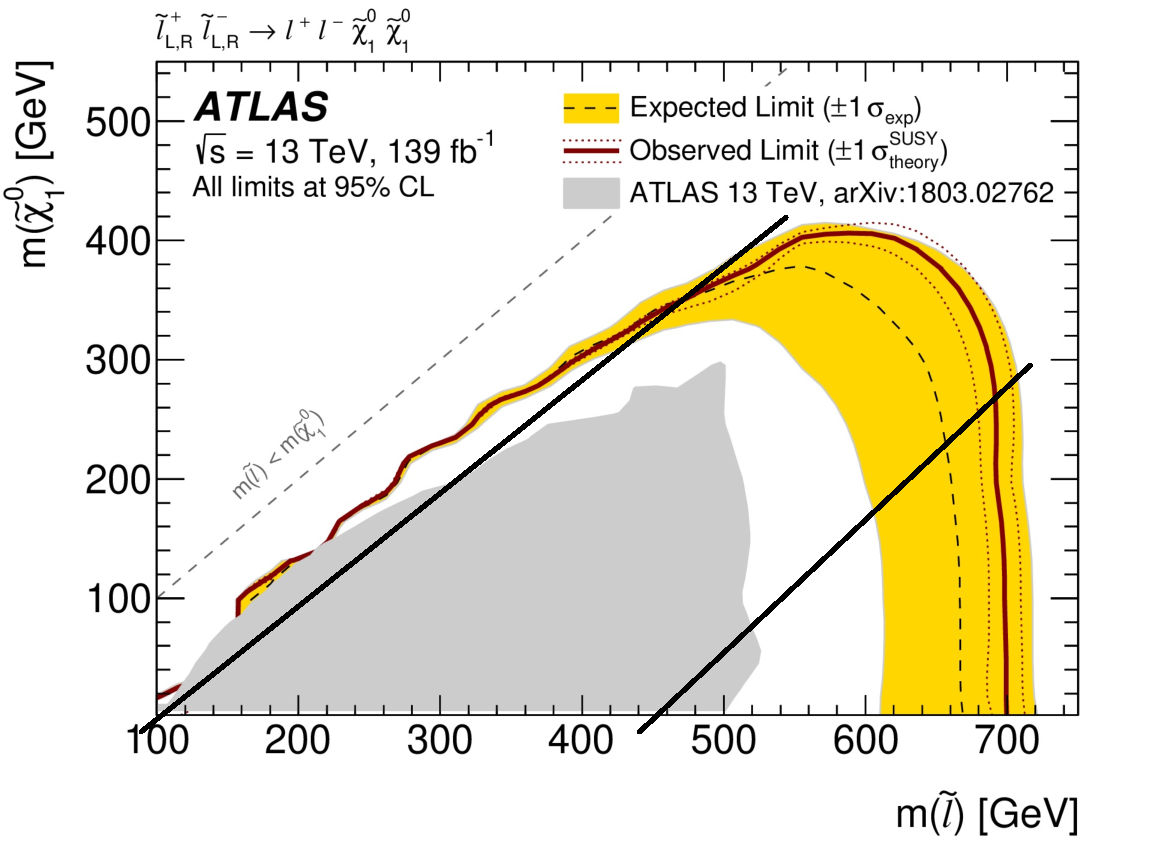
\includegraphics[width = \textwidth]{Figures/FromOnline/Slepslep.pdf}
        \caption{Slepton pair production ($\Tilde{l}\Tilde{l}$) \cite{sleptonexclusion}.}
        \label{fig:slepslepexclusion}
    \end{subfigure}
    \begin{subfigure}[t!]{0.49\textwidth}
        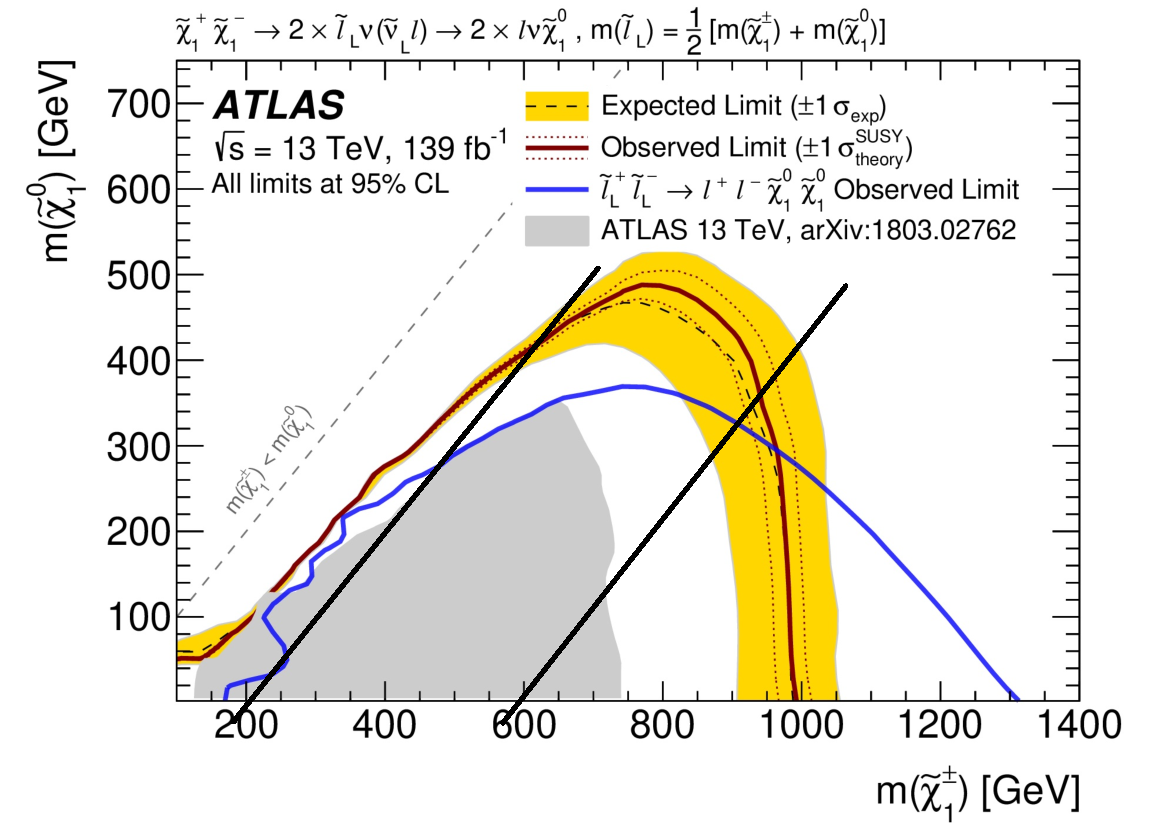
\includegraphics[width = \textwidth]{Figures/FromOnline/Slepsnu.pdf}
        \caption{$\chi_1^+ \chi_1^-$ production via $\Tilde{l}/\Tilde{\nu}$ \cite{sleptonexclusion}.}
        \label{fig:slepsnuexclusion}
    \end{subfigure}
    \\
    \begin{subfigure}[t!]{0.49\textwidth}
        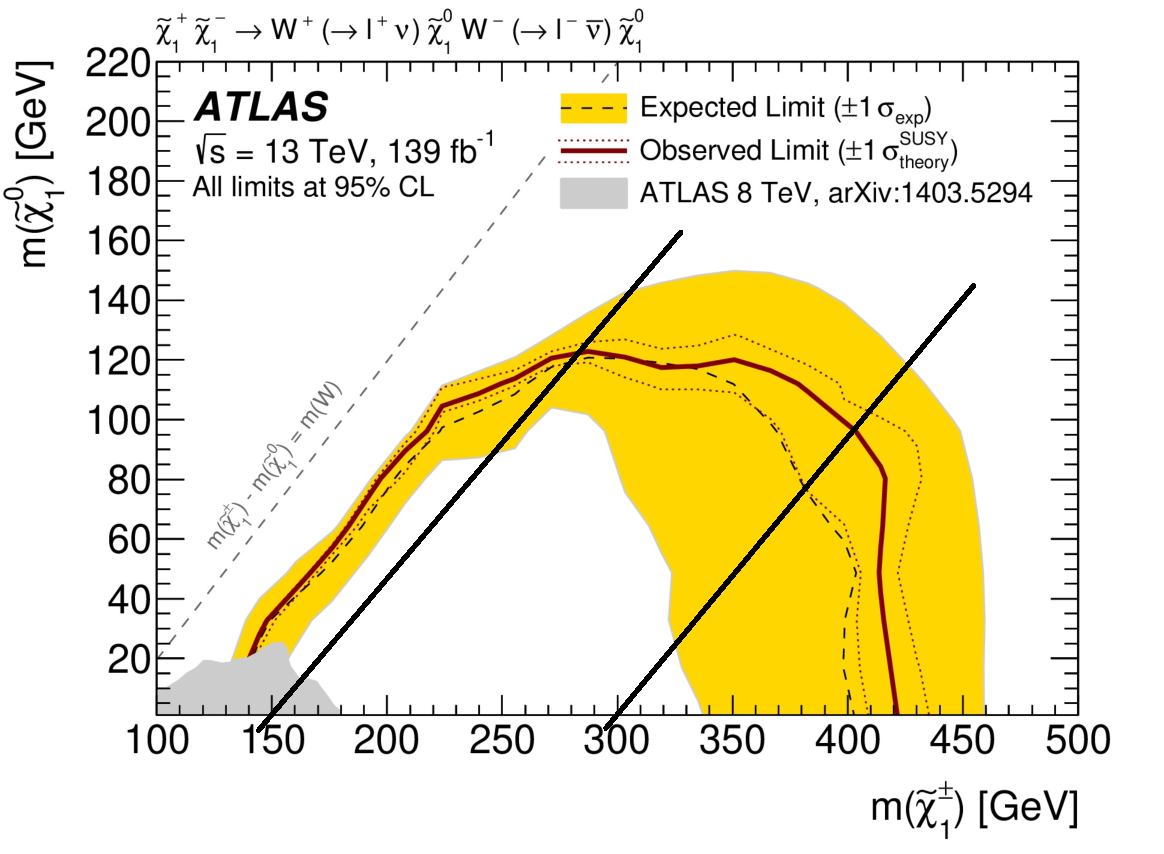
\includegraphics[width = \textwidth]{Figures/FromOnline/WW.pdf}
        \caption{$\chi_1^+ \chi_1^-$ production via W-boson \cite{sleptonexclusion}.}
        \label{fig:WWexclusion}
    \end{subfigure}
    \begin{subfigure}[t!]{0.49\textwidth}
        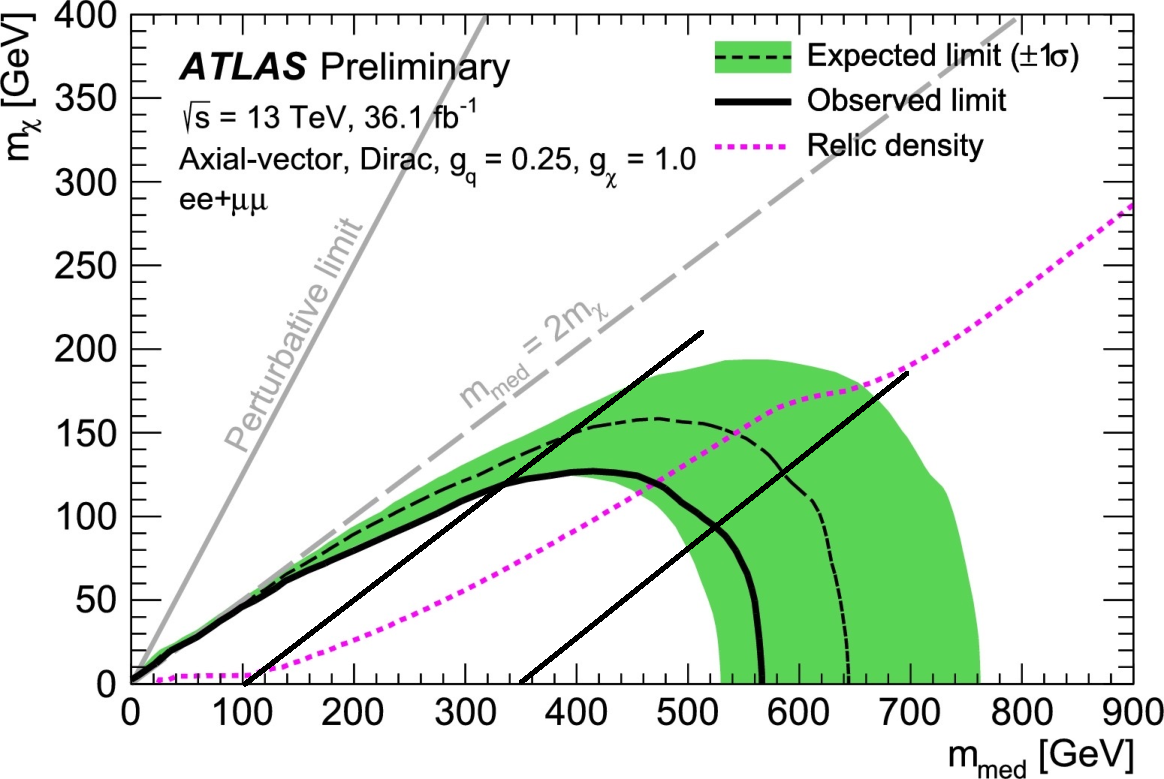
\includegraphics[width = \textwidth]{Figures/FromOnline/mono_Z.pdf}
        \caption{Mono-Z process \cite{monoZexclusion}.}
        \label{fig:monoZexclusion}
    \end{subfigure}
    \caption{The observed and expected exclusion limits for both the SUSY simplified models in \ref{fig:slepslepexclusion}, \ref{fig:slepsnuexclusion} and \ref{fig:WWexclusion} and for the DM model in \ref{fig:monoZexclusion}. The lines drawn in the plot is to show the mass splittings for each process.}
    \label{fig:exclusionPlots}
\end{figure}

The two black lines in each plot in figure \ref{fig:exclusionPlots} shows the division of the signal samples into different mass splittings in the ML analysis later in the thesis. To compare our ML results with the cut and count analysis, we have chosen one representative signal sample from each part of the plots in figure \ref{fig:exclusionPlots}. This gives us the signal samples listed in table \ref{tab:sigsampcutandcount}.

\begin{table}[H]
    \centering
    \begin{tabular}{c c c c}
    \toprule
    \textbf{m}$\mathbf{(\Tilde{l}, \Tilde{\chi}_1^0)}$ & \textbf{m}$\mathbf{(\Tilde{\chi}_1^\pm, \Tilde{\chi}_1^0)}$ & \textbf{m}$\mathbf{(\Tilde{\chi}_1^\pm, \Tilde{\chi}_1^0)}$ & \textbf{m}$\mathbf{( V, \chi)}$  \\
    \midrule
    \midrule
    (400, 300) & (300, 200) & (150, 25) & (150, 80)\\
    (600, 300) & (800, 400) & (350, 100) & (400, 150)\\
    (700, 1) & (1000, 100) & (425, 25) & (650, 1)\\
    \bottomrule
    \end{tabular}
    \caption{An overview of the masses of the signals that are used for this thesis.}
    \label{tab:sigsampcutandcount}
\end{table}

These signal samples are going to follow us through both analysis (cut and count and ML). They are also shown in figure \ref{fig:cutandcountMONA} where we have followed the same procedure as the ATLAS publications. The main difference between the publications and our results is that we have chosen some other signal samples than the publications. The reason for this is because we want to have one benchmark signal from each mass splitting made from looking at figure \ref{fig:exclusionPlots}. The publications have $m(\Tilde{l}, \Tilde{\chi}_1^0) = (400, 200)$ GeV, $m(\Tilde{\chi}_1^\pm, \Tilde{\chi}_1^0) = (300, 50)$ GeV, $m(\Tilde{\chi}_1^\pm, \Tilde{\chi}_1^0) = (600, 300)$ GeV and $m(V, \chi) = (500,100)$ GeV. Since we have chosen to look at different signal samples than the publications \cite{sleptonexclusion, monoZexclusion}, we have to see if the backgrounds for all four processes are compatible. 


In figure \ref{fig:cutandcountMONA} we can see our final results for the same variables as in the publications, from the cut and count analysis.

\newgeometry{twoside,inner=3cm,outer=2cm}
\begin{figure}[H]
%\begin{minipage}{2\textwidth}
%\begin{adjustwidth}{-3cm}{-3cm}
\centering
%\advance\leftskip-4cm 
%\advance\rightskip-4cm 
    \begin{subfigure}[t!]{0.49\textwidth}
        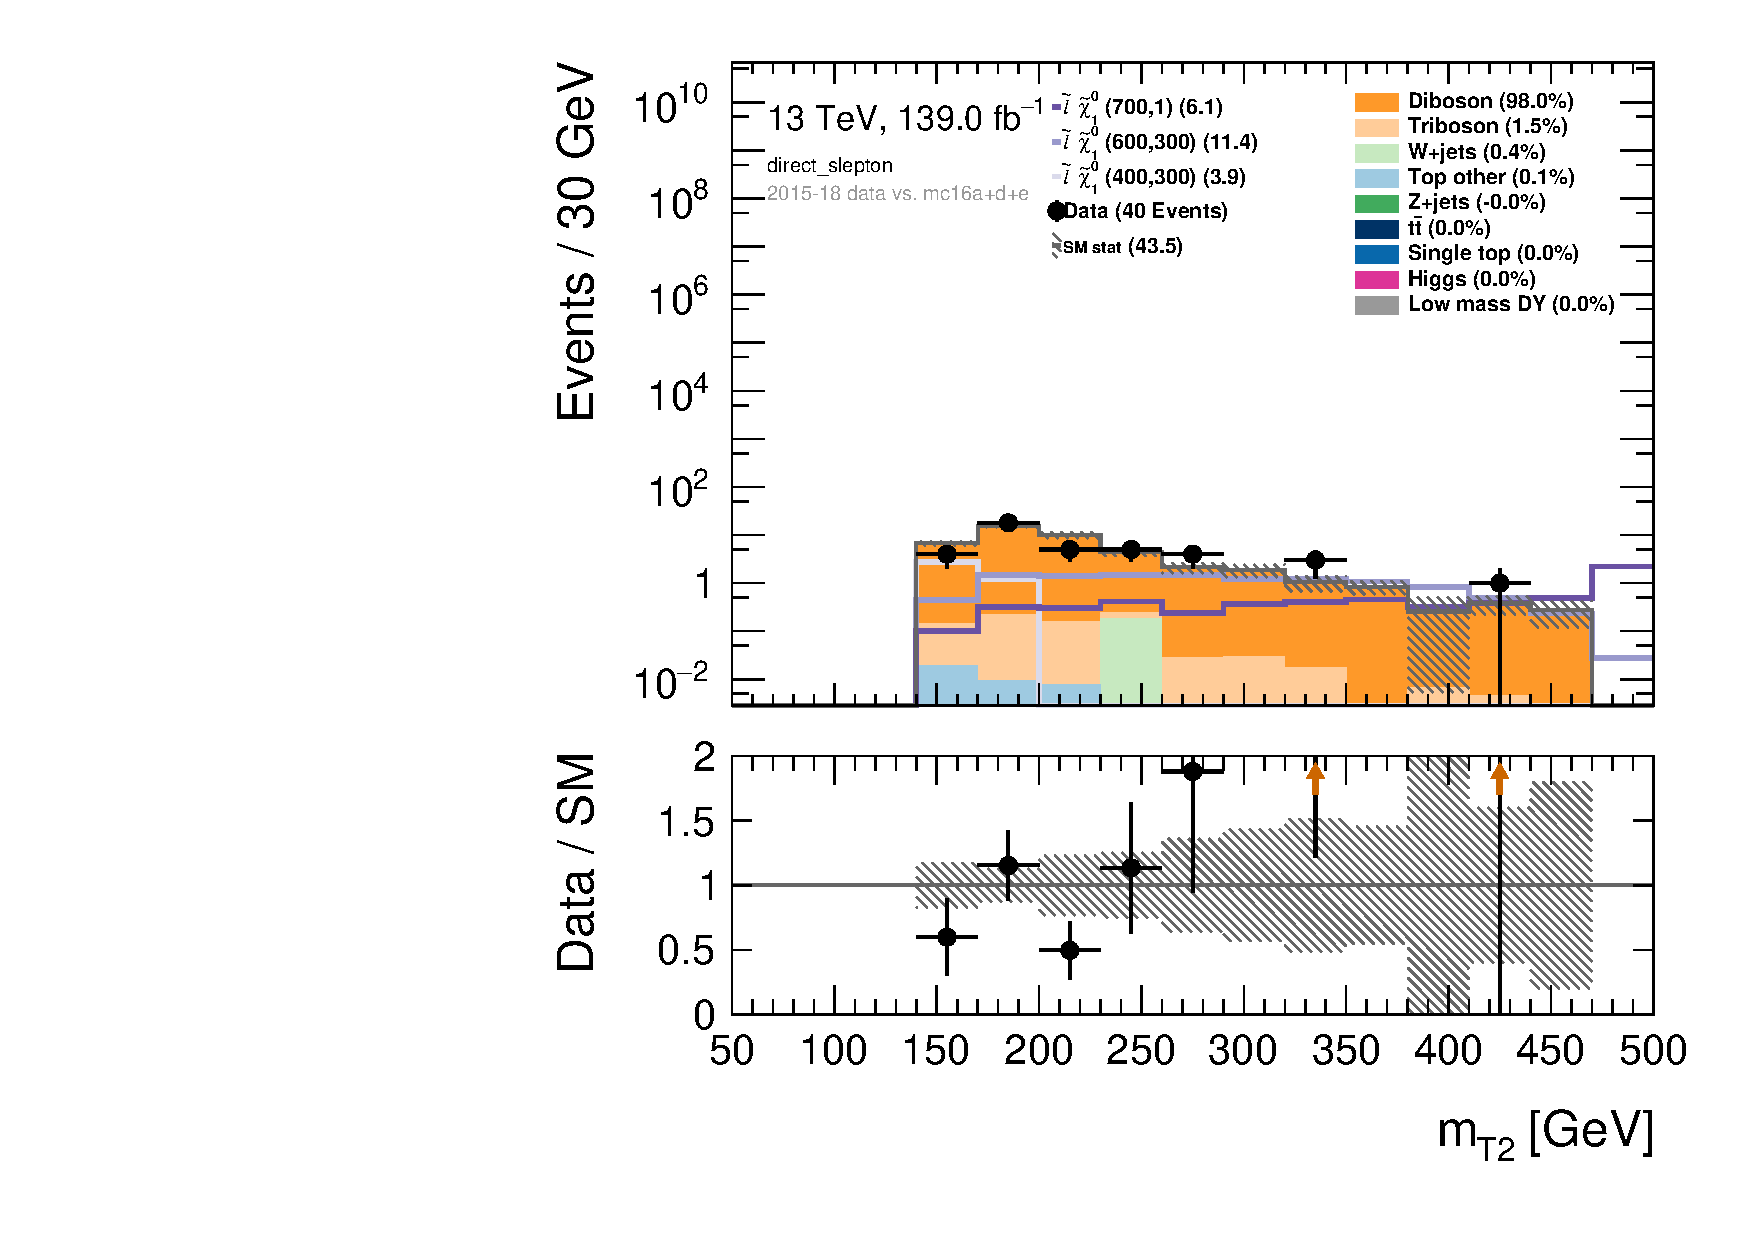
\includegraphics[width=\textwidth]{Figures/cutandcount/hist1d_mt2_direct_slepton.pdf}
    \caption{Stransverse mass for direct slepton production.}
    \label{fig:cutandcountslepslep}
    \end{subfigure}
    \begin{subfigure}[t!]{0.49\textwidth}
        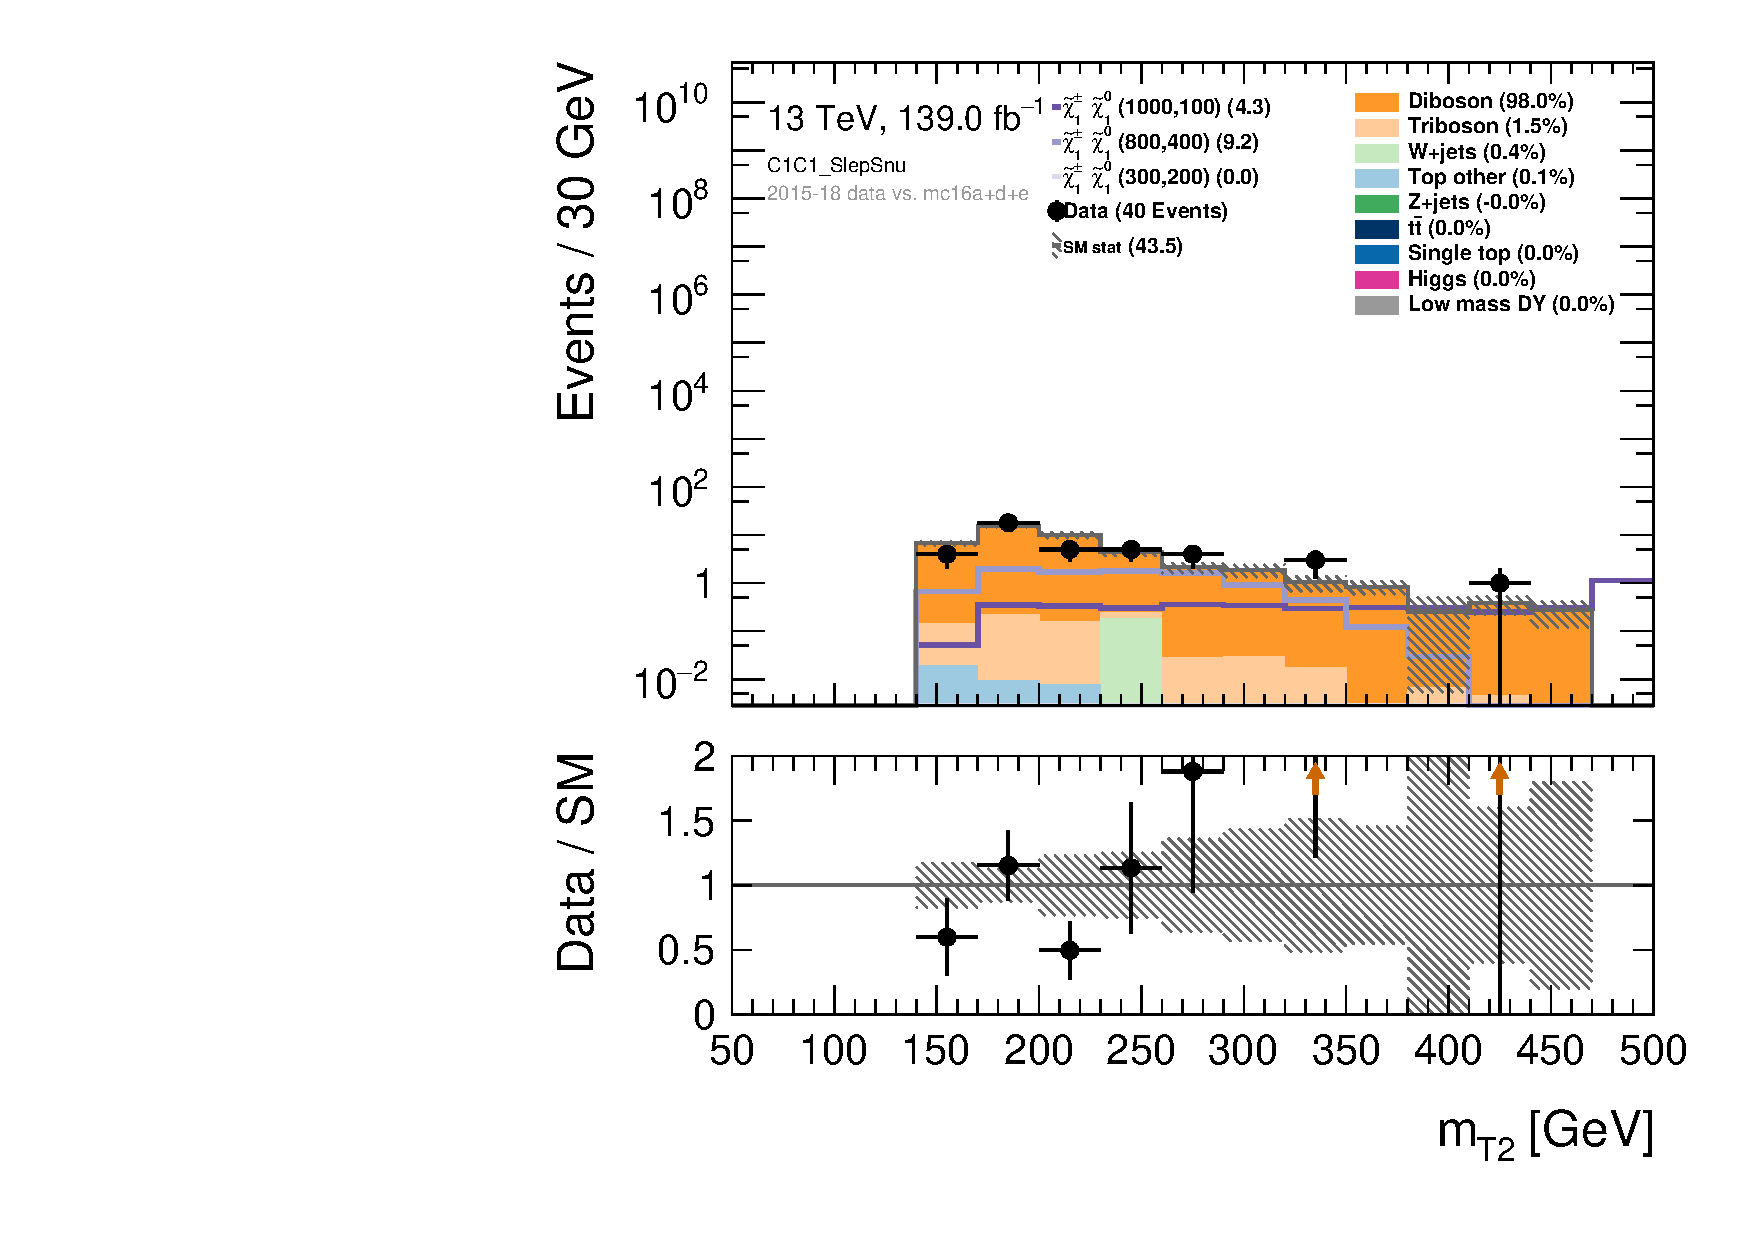
\includegraphics[width=\textwidth]{Figures/cutandcount/hist1d_mt2_C1C1_SlepSnu.pdf}
    \caption{Stransverse mass for chargino production via $\Tilde{l}/\Tilde{\nu}$.}
    \label{fig:cutandcountslepsnu}
    \end{subfigure}
    \\
    \begin{subfigure}[t!]{0.49\textwidth}
        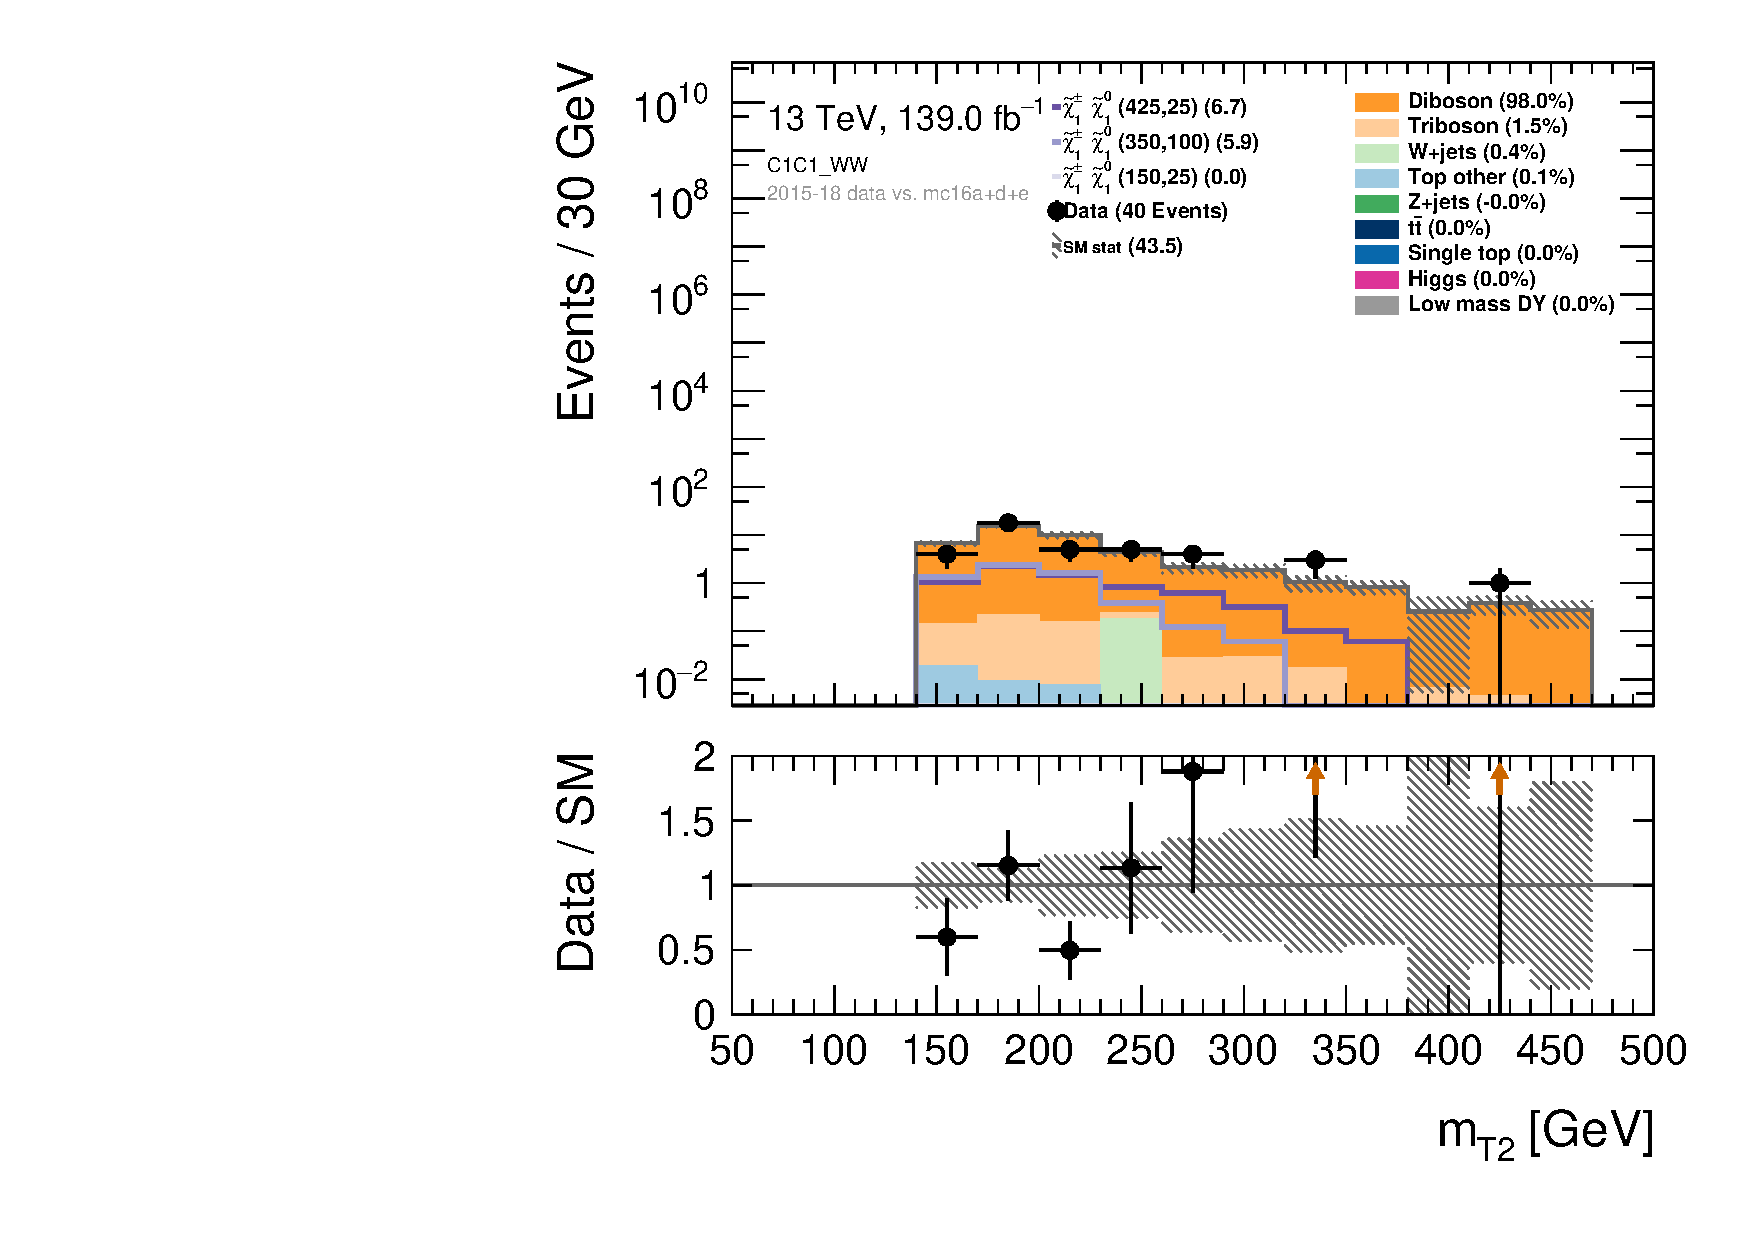
\includegraphics[width=\textwidth]{Figures/cutandcount/hist1d_mt2_C1C1_WW.pdf}
    \caption{Stransverse mass for chargino production via $W^\pm$.}
    \label{fig:cutandcountWW}
    \end{subfigure}
    \begin{subfigure}[t!]{0.49\textwidth}
        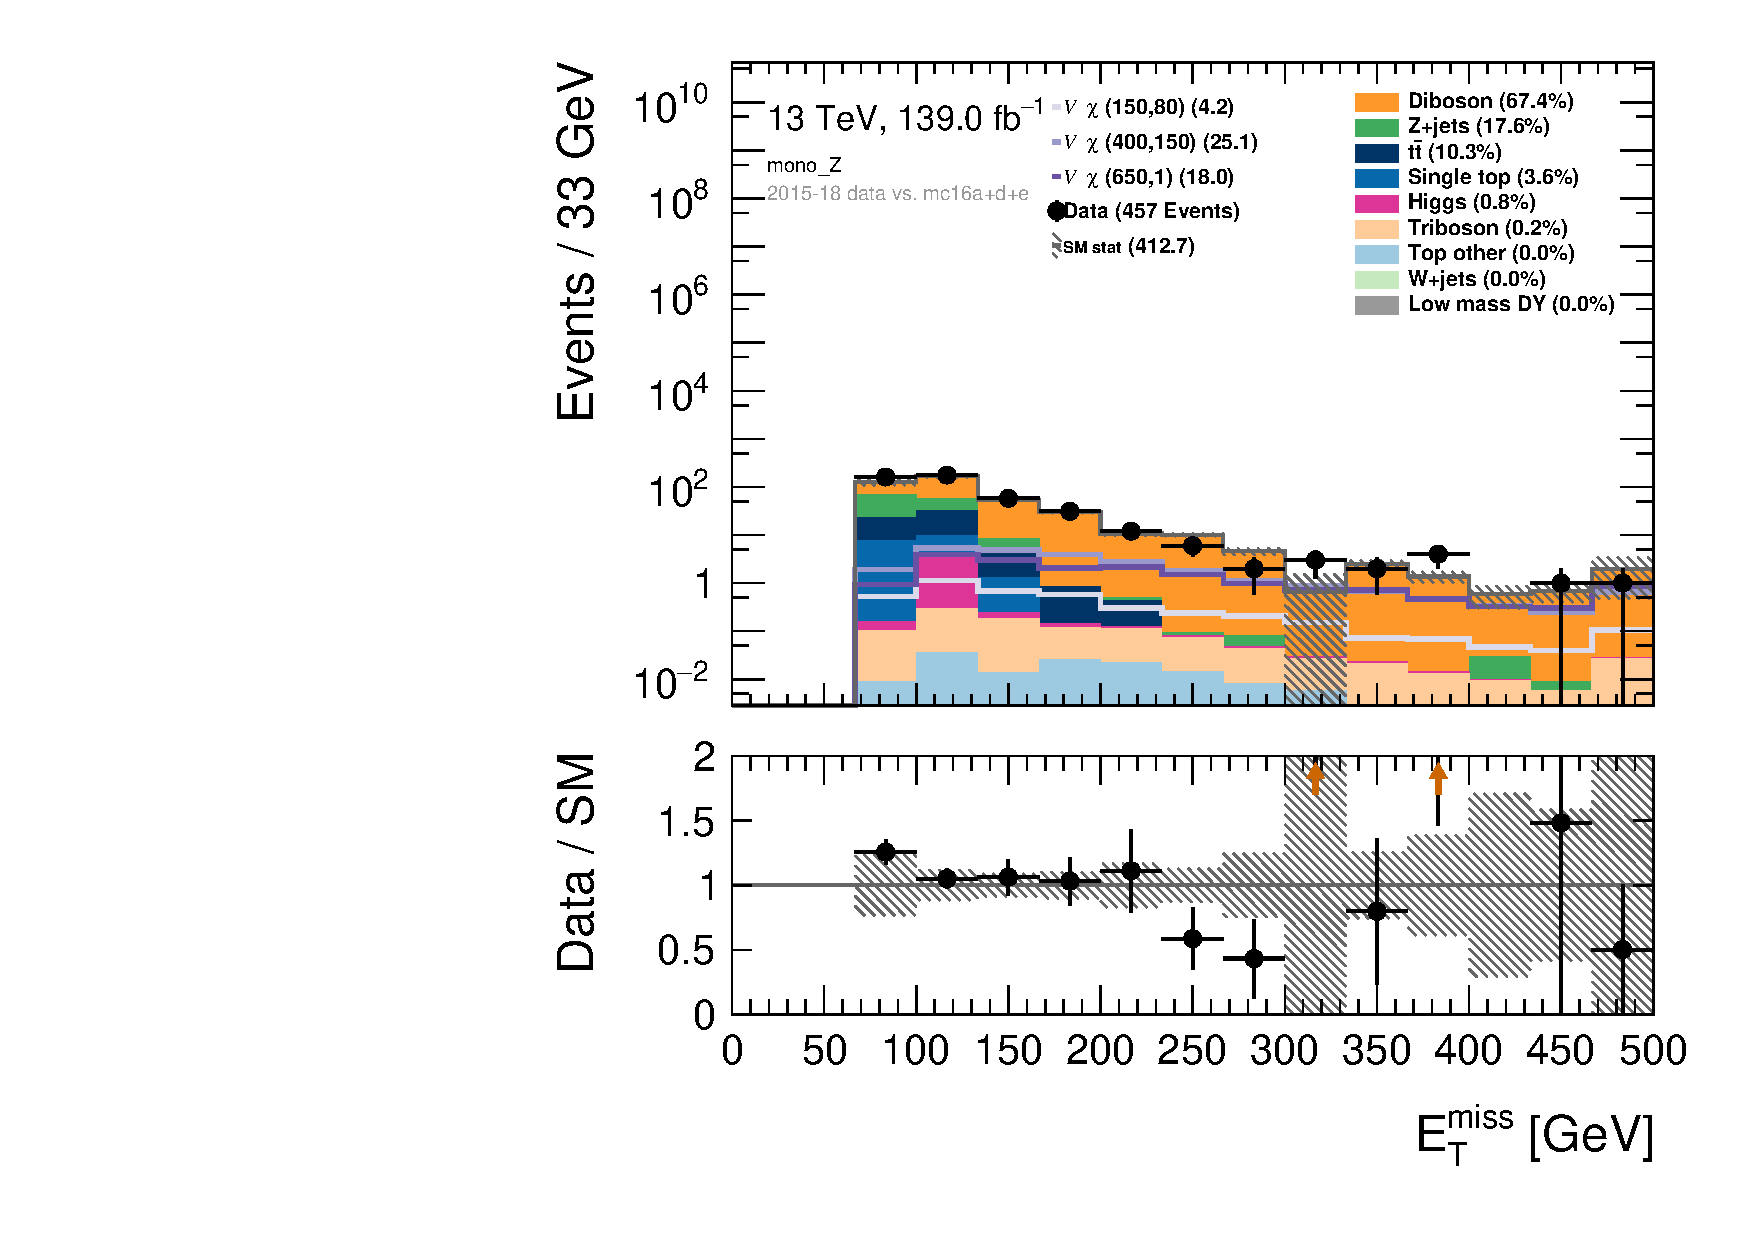
\includegraphics[width=\textwidth]{Figures/cutandcount/hist1d_met_Et_mono_Z.pdf}
    \caption{Missing transverse energy for mono-Z.}
    \label{fig:cutandcountmonoZ}
    \end{subfigure}
    \caption{Results from the cut and count analysis for all four processes, where we have followed the same procedure as the publications done by ATLAS.}
    \label{fig:cutandcountMONA}
\end{figure}
\restoregeometry


In figure \ref{fig:cutandcountMONA} we can see that for the direct slepton production and for the chargino production with slepton/sneutrino-mediated-decay we are able to separate some signal samples from the background in the high end of the $m_{T_2}$ variable. In \ref{fig:cutandcountslepslep} both the high and intermediate mass splitting samples are separated from the background and could lead to detection. In \ref{fig:cutandcountslepsnu} only the high mass splitting sample is above the background and could be possible to detect. While for the chargino production with W-boson-mediated-decay and mono-Z we have not been able to separate the signal from the background. In comparison to the results from the publications (shown in figure \ref{fig:atlaspub}), we can see that we have roughly the same amount of events in the different bins and can therefore conclude with that they are compatible and we have managed to reproduce the published results.

Now we are going to move on to the ML part, which is the main part of this thesis, and see if we can do the same analysis with some different tools. In the end we will compare the results obtained in this chapter to see if ML can do a better separation than we have managed to do with cut and count. Before presenting the ML results in chapter \ref{sec:MLanalysis}, we first give an introduction to Machine Learning in chapter \ref{sec:ML}.


























\begin{comment}
%The first part of this analysis was done by cut and count. Here I have plotted four different variables which also represent some of the features used in the ML part. To demonstrate how the cut and count method behaves I have plotted each variable after adding a group of cuts. In the following figures you can see an example of this for the direct slepton production. You can also find examples of this for the charginos via slepton/sneutrino and via W-bosons in the appendix(OR GITHUB REPO??????). These two processes behave very similarly to the direct slepton production so I have chosen to show only one of them. 

%In the first figure \ref{fig:slepslep1stcut} we can see the whole mass distribution for the SM background with the final state two leptons with opposite charge. We can see that Z-jets is definitely the dominating background and by adding some cuts we can reduce this background.


\begin{figure}[H]
%\begin{minipage}{2\textwidth}
%\begin{adjustwidth}{-3cm}{-3cm}
\centering
%\advance\leftskip-4cm 
%\advance\rightskip-4cm 
    \begin{subfigure}[t!]{0.49\textwidth}
        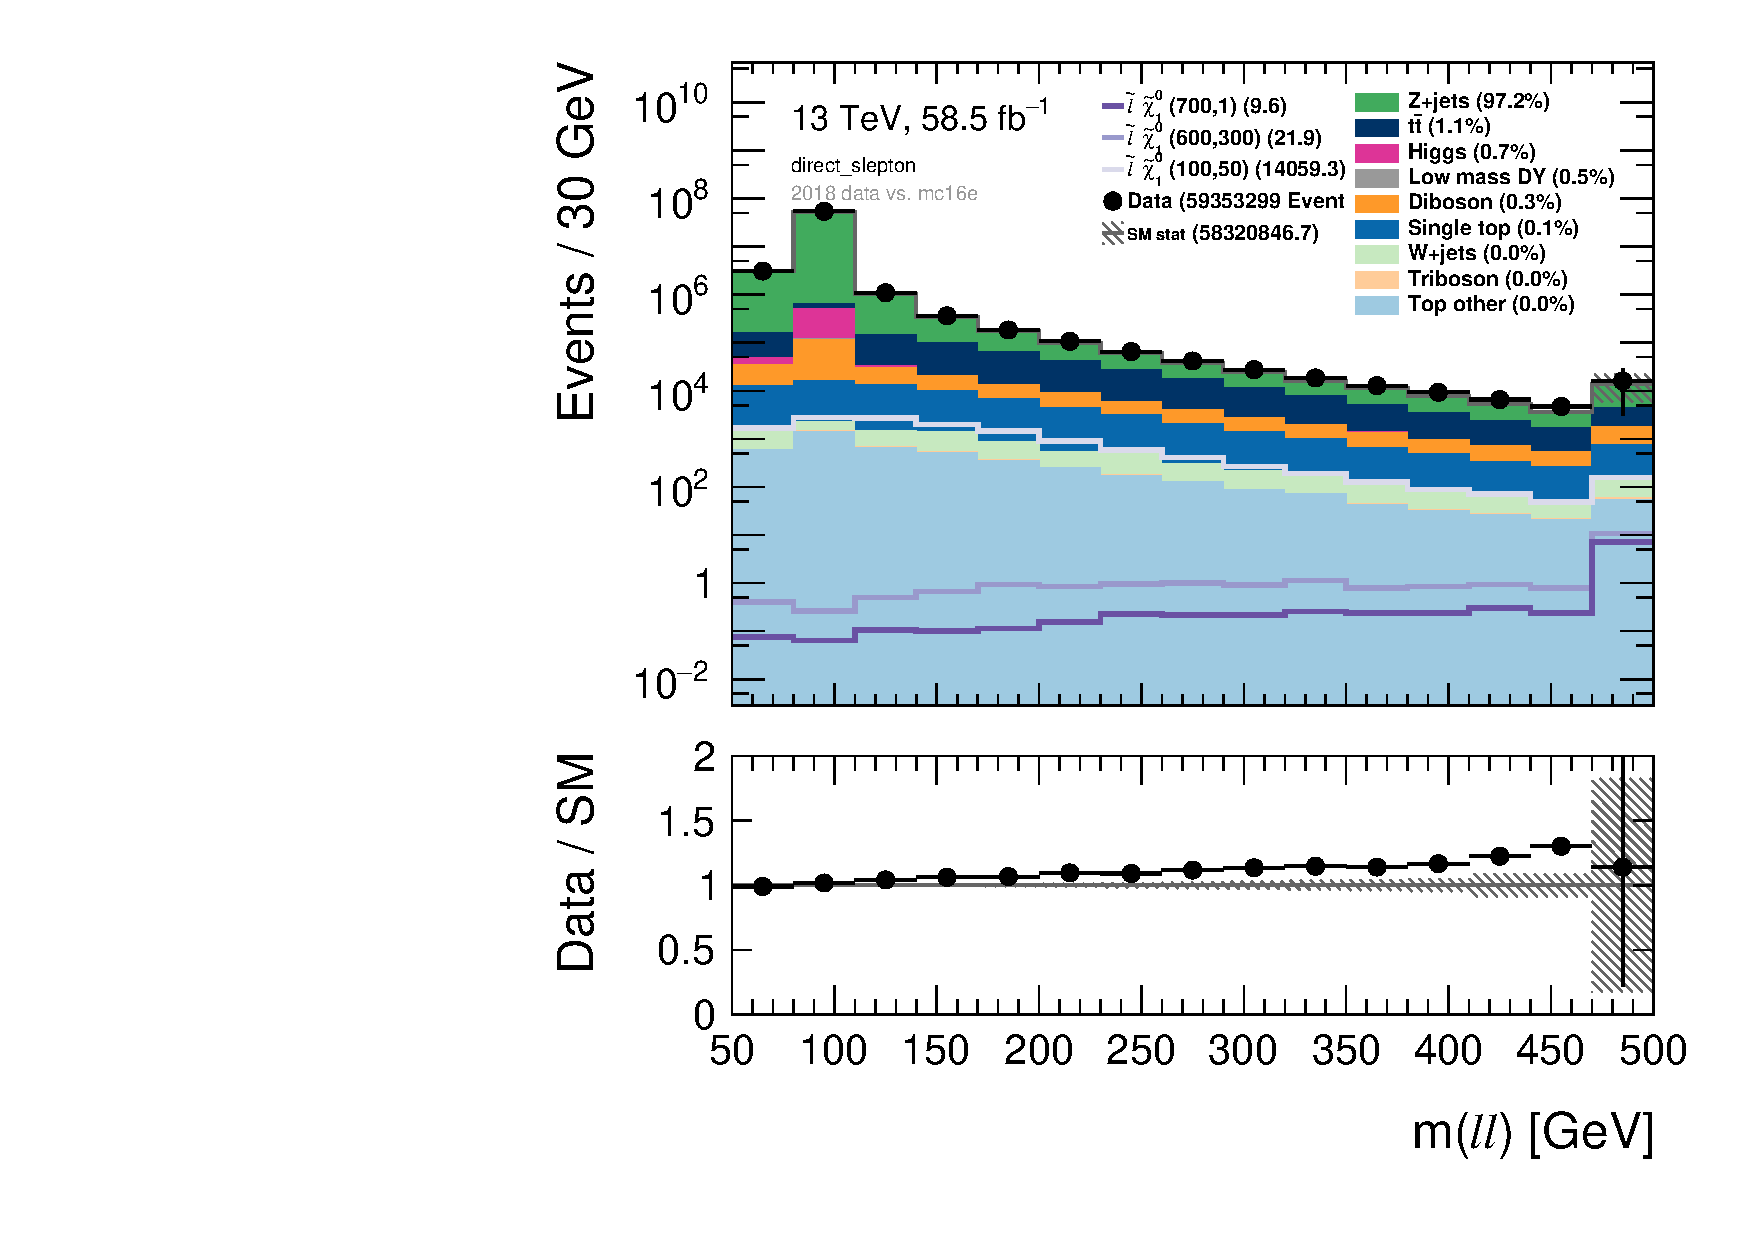
\includegraphics[width=\textwidth]{Figures/SlepSlep/CutAndCount/1stcut_2L+OS/hist1d_mll_direct_slepton.pdf}
    \caption{Invariant mass}
    \label{fig:my_label}
    \end{subfigure}
    \begin{subfigure}[t!]{0.49\textwidth}
        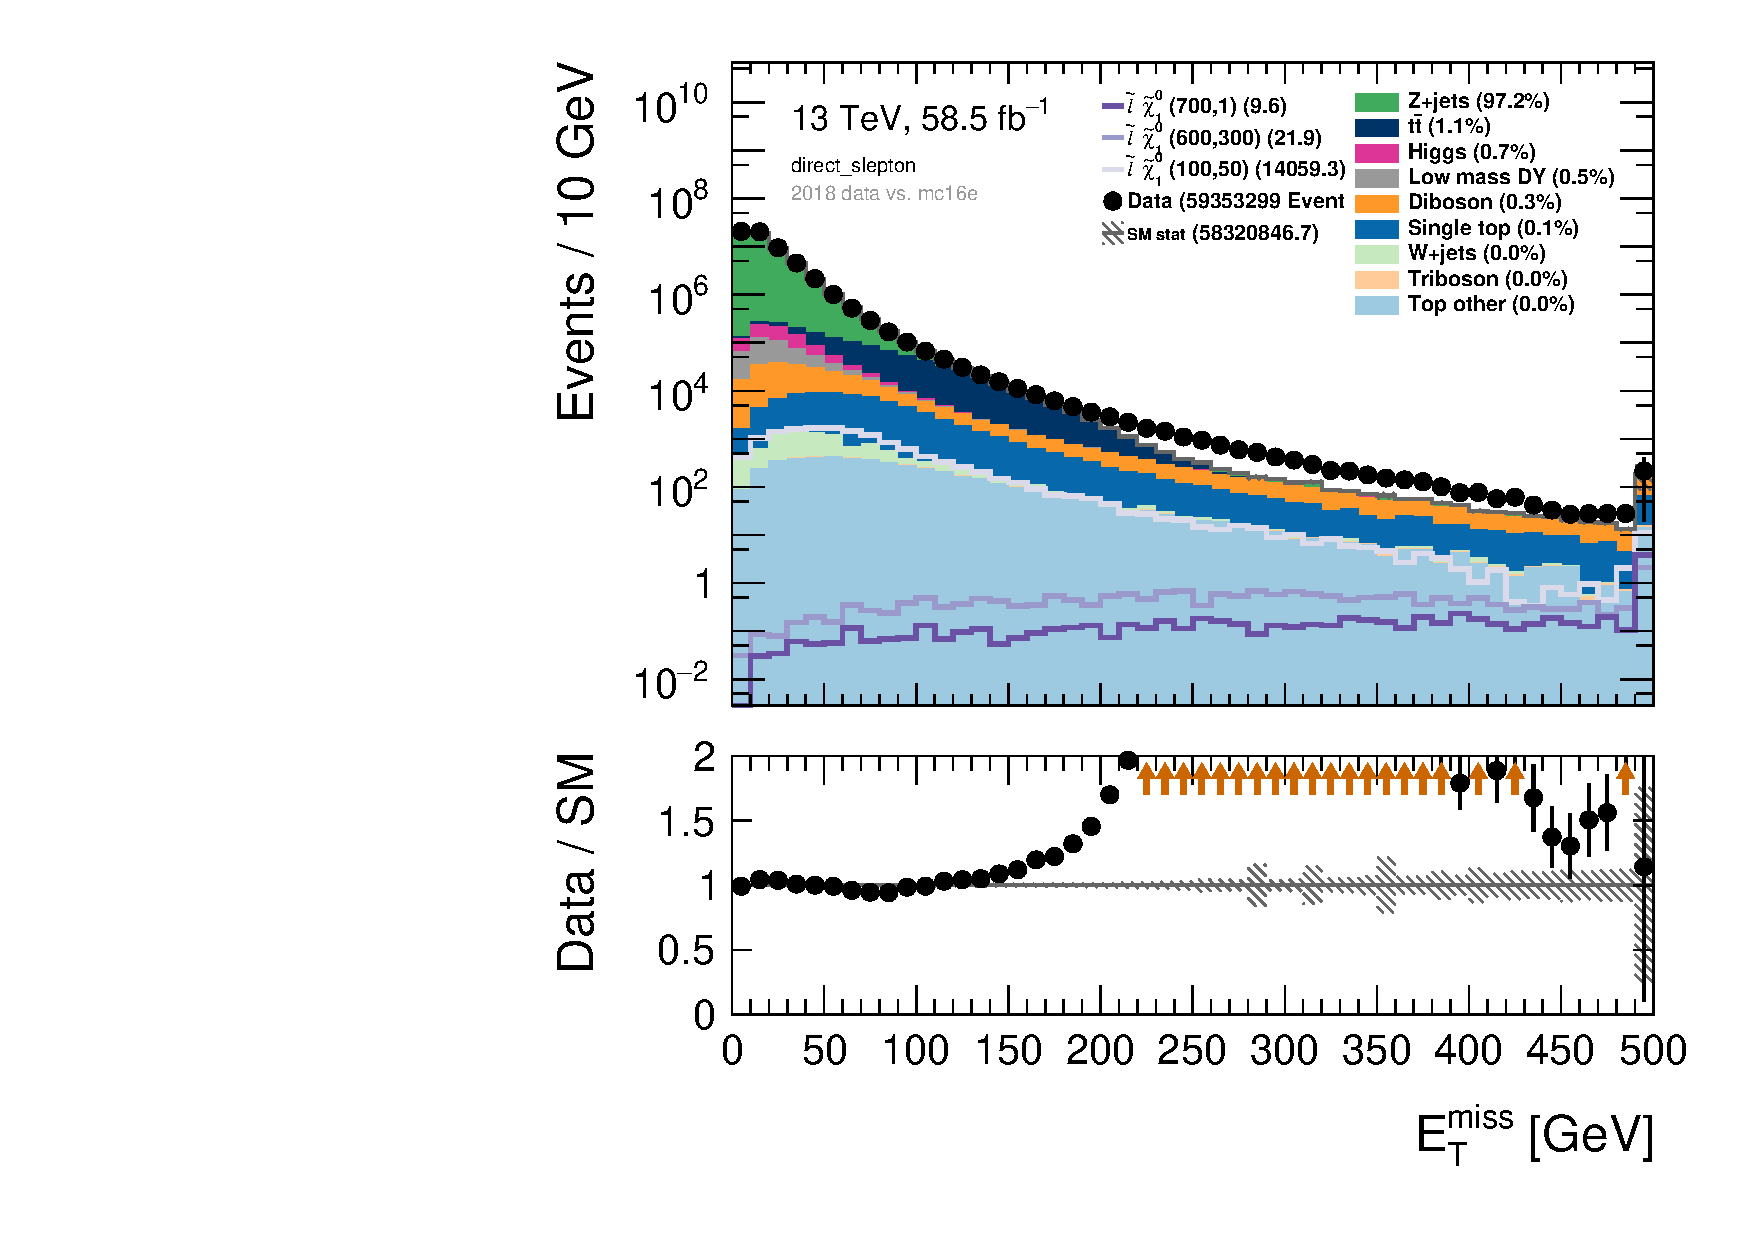
\includegraphics[width=\textwidth]{Figures/SlepSlep/CutAndCount/1stcut_2L+OS/hist1d_met_Et_direct_slepton.pdf}
    \caption{Missing transverse energy}
    \label{fig:my_label}
    \end{subfigure}
    \\
    \begin{subfigure}[t!]{0.49\textwidth}
        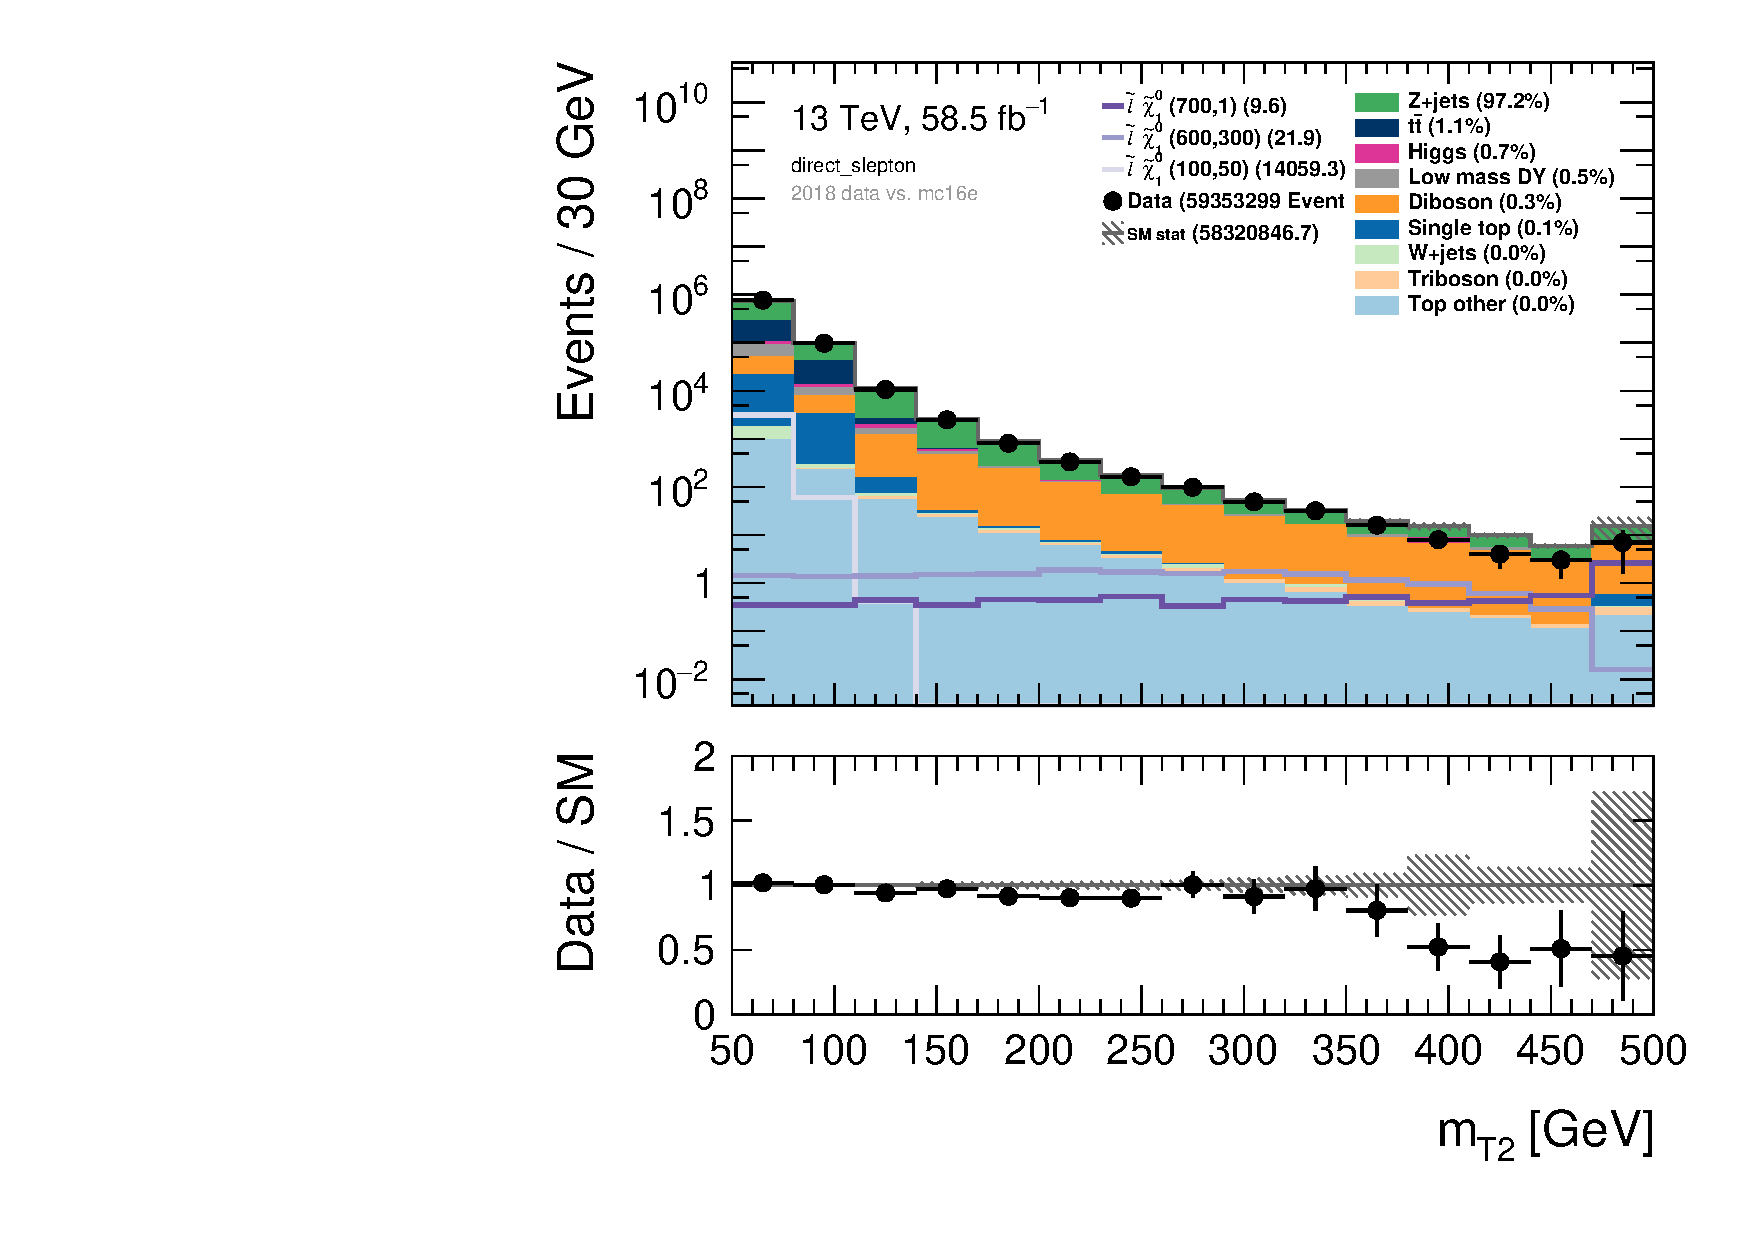
\includegraphics[width=\textwidth]{Figures/SlepSlep/CutAndCount/1stcut_2L+OS/hist1d_mt2_direct_slepton.pdf}
    \caption{Stransverse mass}
    \label{fig:my_label}
    \end{subfigure}
    \begin{subfigure}[t!]{0.49\textwidth}
        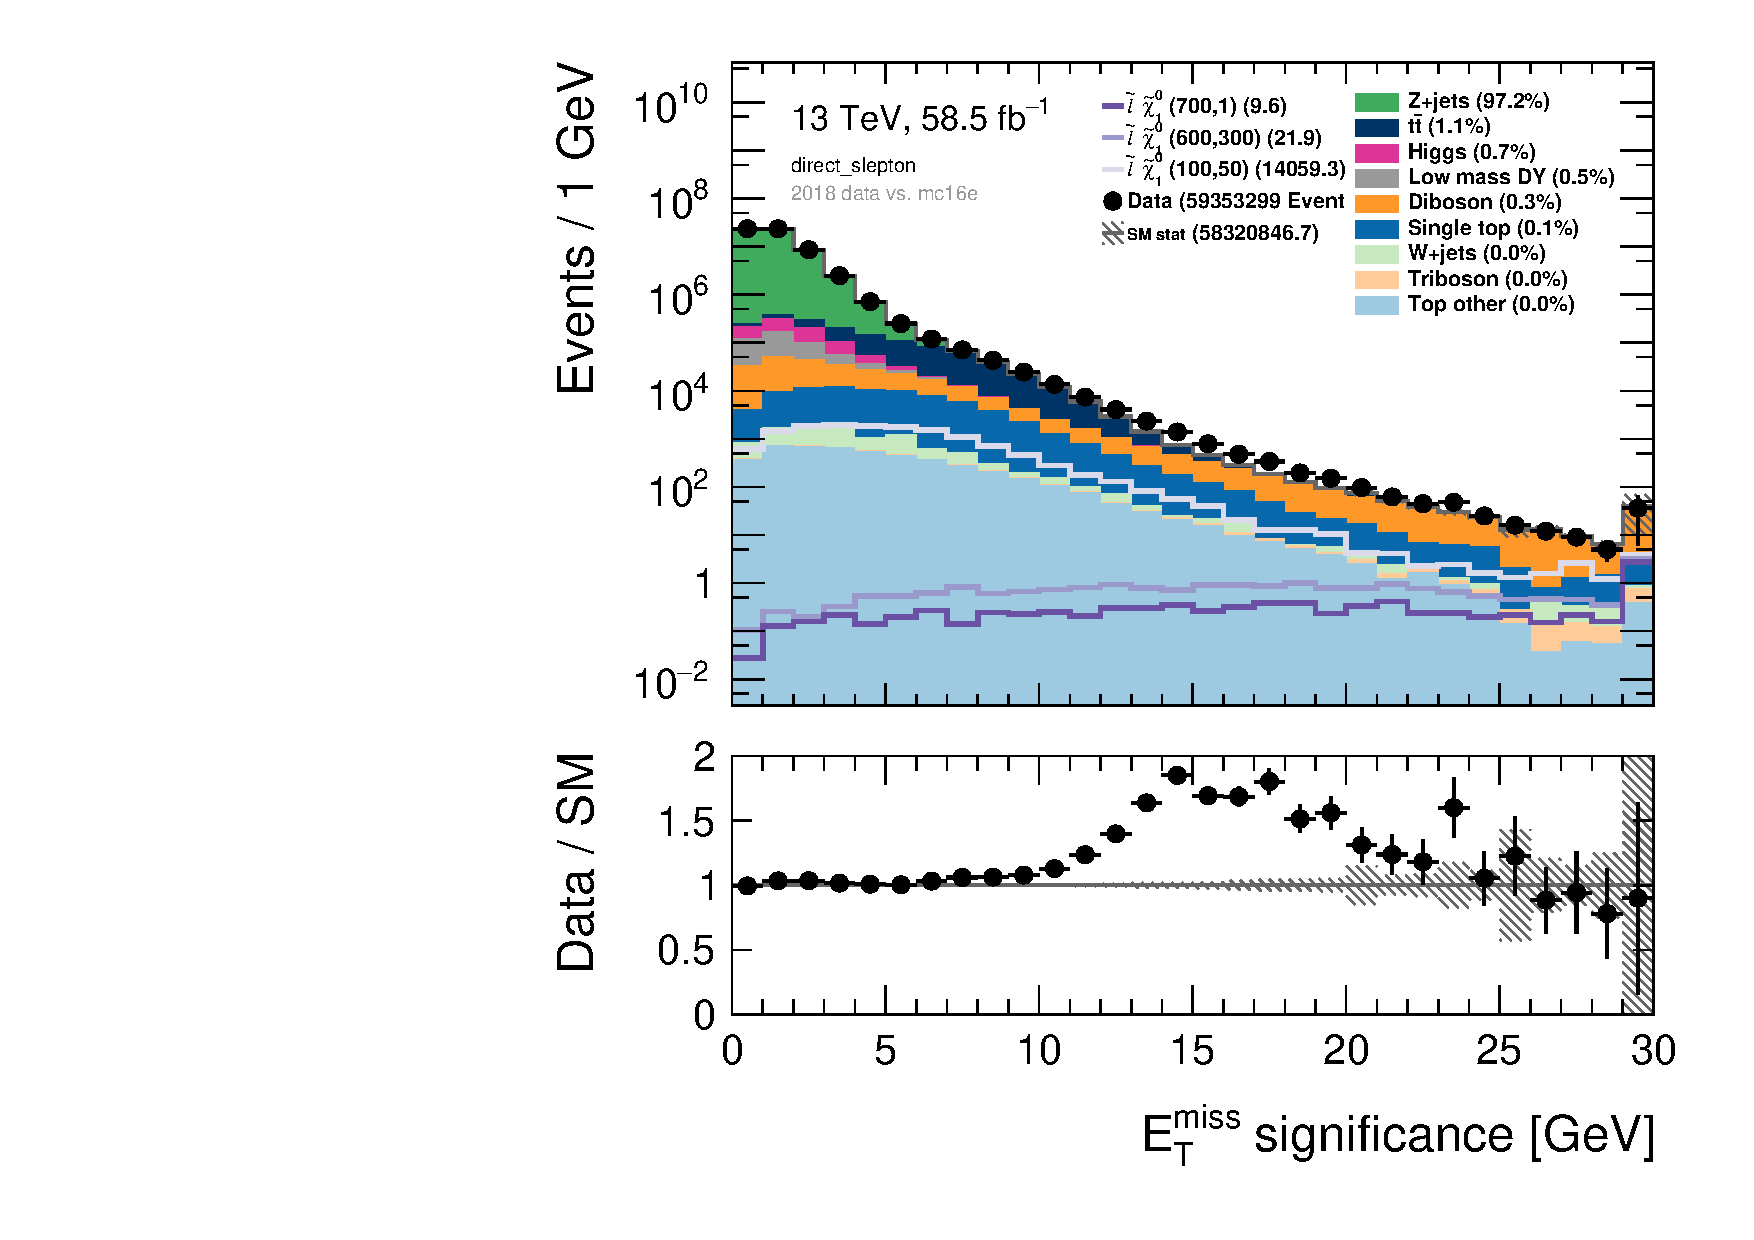
\includegraphics[width=\textwidth]{Figures/SlepSlep/CutAndCount/1stcut_2L+OS/hist1d_met_Sign_direct_slepton.pdf}
    \caption{Missing transverse energy significance}
    \label{fig:my_label}
    \end{subfigure}
    \caption{Plot of the four most important variables in direct slepton production with a cut on only two leptons with opposite charge in the final state.}
    \label{fig:slepslep1stcut}
\end{figure}


After adding a met cut and doing a Z-veto we get the results in figure \ref{fig:slepslep3rdcut} where we can see that Z + jets is reduced a lot. For most of the variables we can now see that the $t\Bar{t}$ is the dominating background, but the signal is still below the backgrounds so we need to add some more cuts.

\begin{figure}[H]
%\begin{minipage}{2\textwidth}
%\begin{adjustwidth}{-3cm}{-3cm}
\centering
%\advance\leftskip-4cm 
%\advance\rightskip-4cm 
    \begin{subfigure}[t!]{0.49\textwidth}
        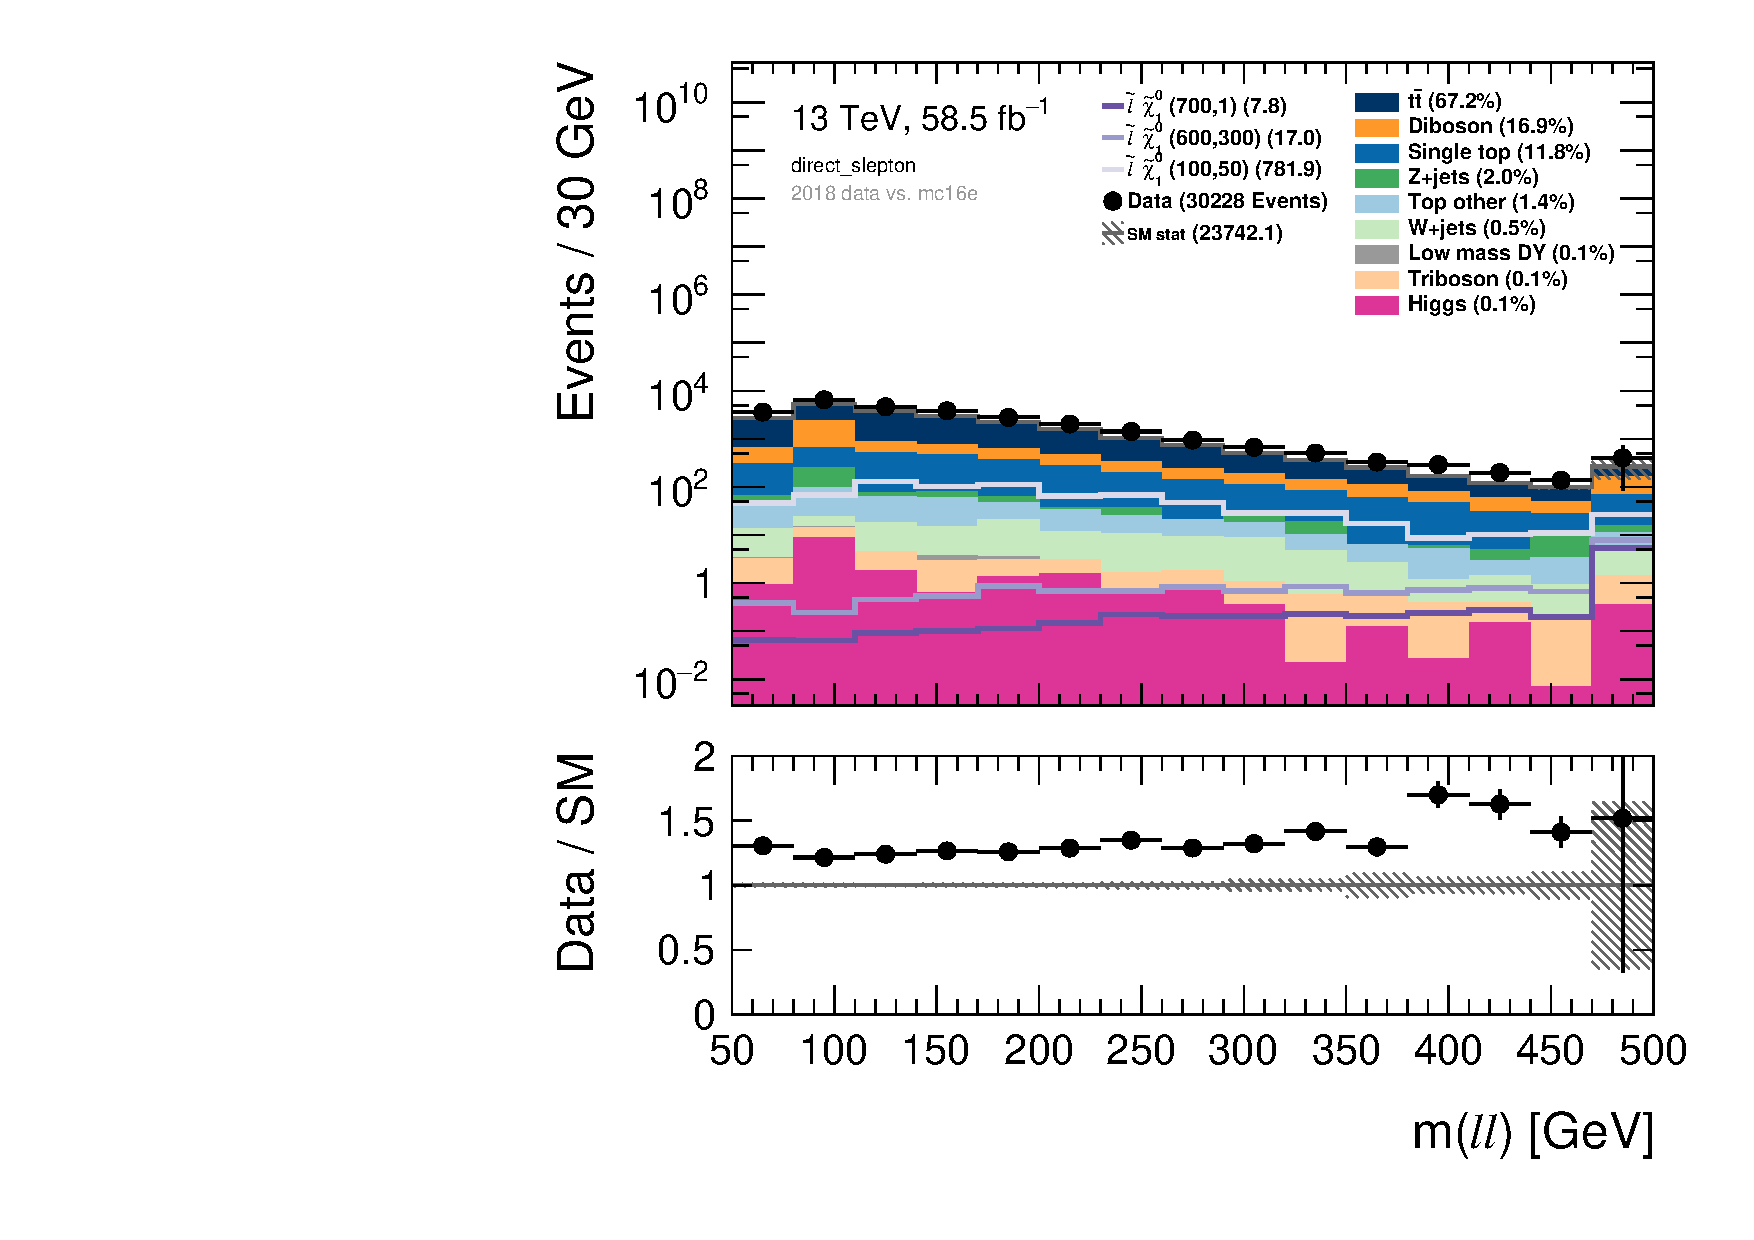
\includegraphics[width=\textwidth]{Figures/SlepSlep/CutAndCount/3rdcut_Zveto/hist1d_mll_direct_slepton.pdf}
    \caption{Invariant mass}
    \label{fig:my_label}
    \end{subfigure}
    \begin{subfigure}[t!]{0.49\textwidth}
        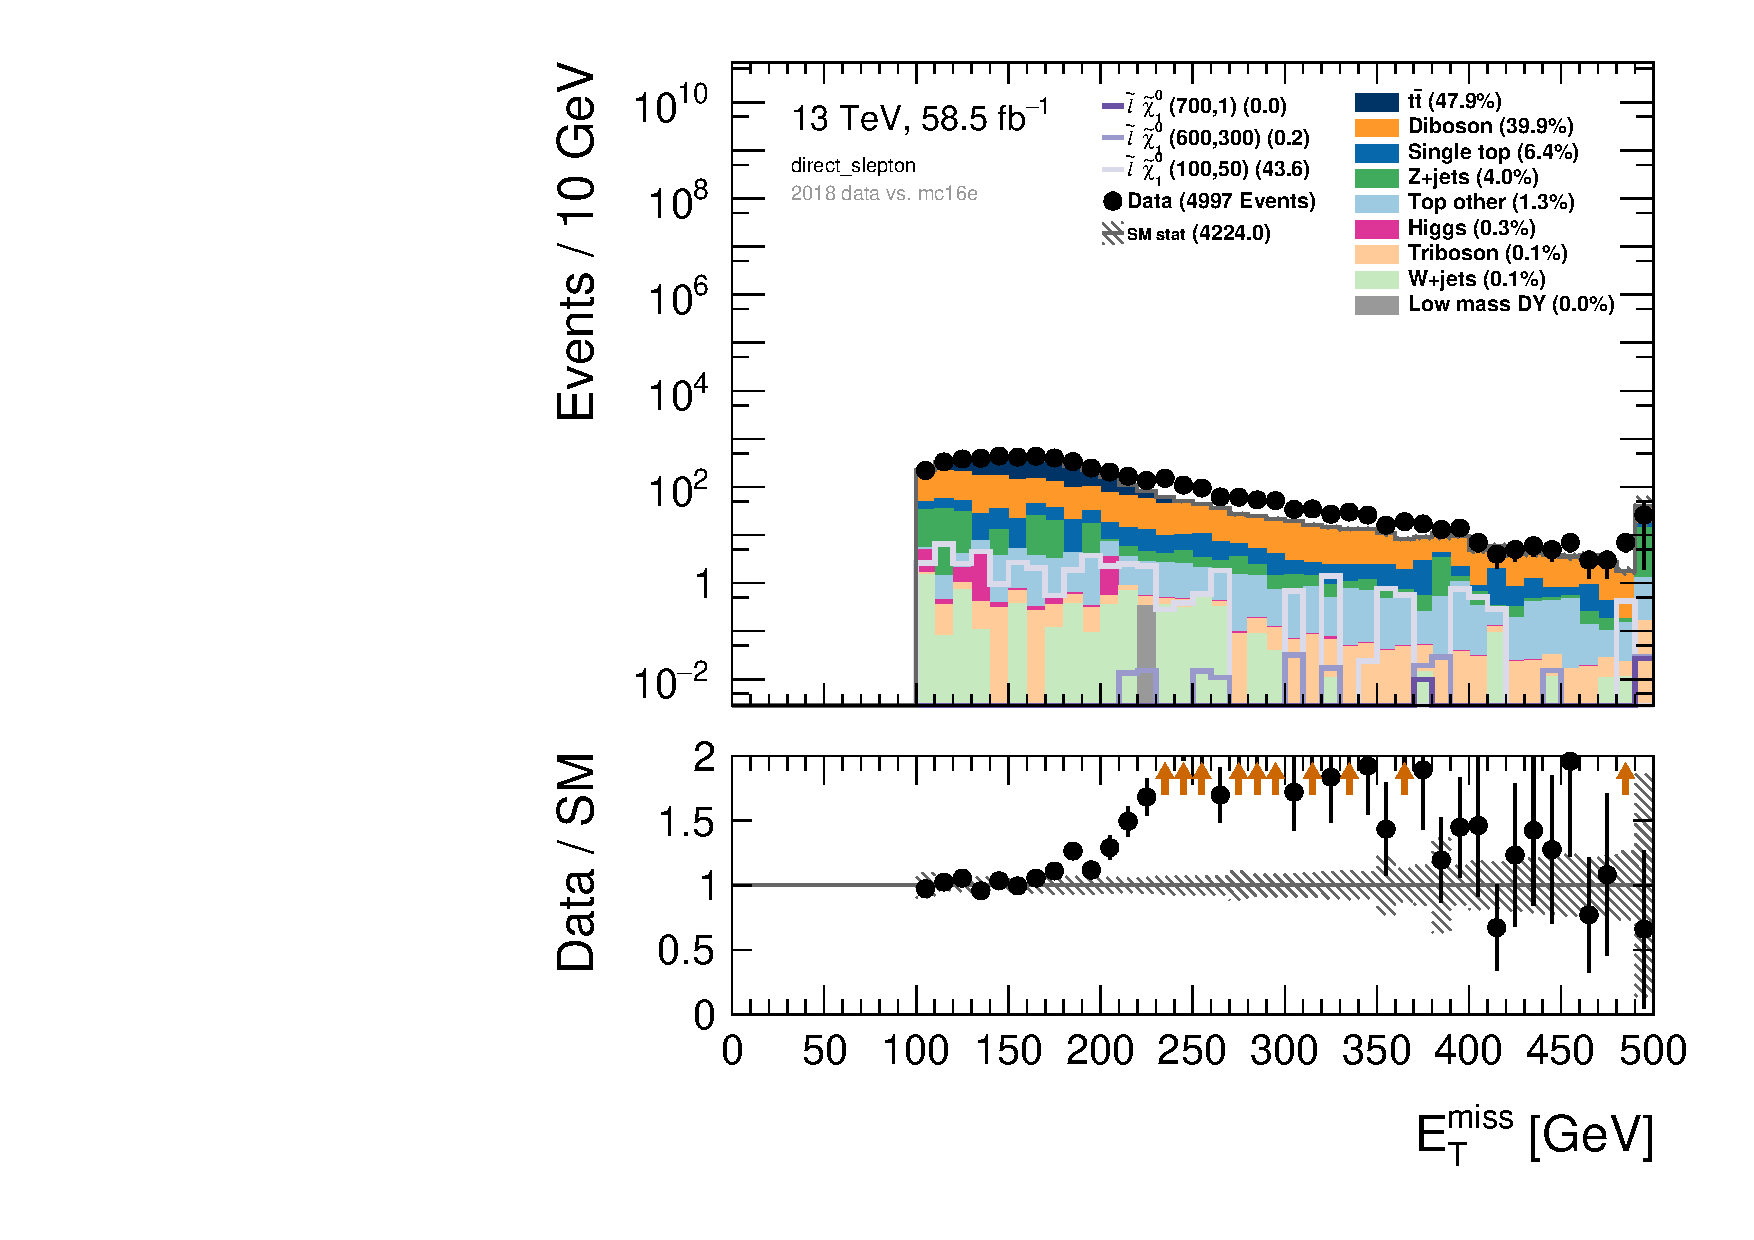
\includegraphics[width=\textwidth]{Figures/SlepSlep/CutAndCount/3rdcut_Zveto/hist1d_met_Et_direct_slepton.pdf}
    \caption{Missing transverse energy}
    \label{fig:my_label}
    \end{subfigure}
    \\
    \begin{subfigure}[t!]{0.49\textwidth}
        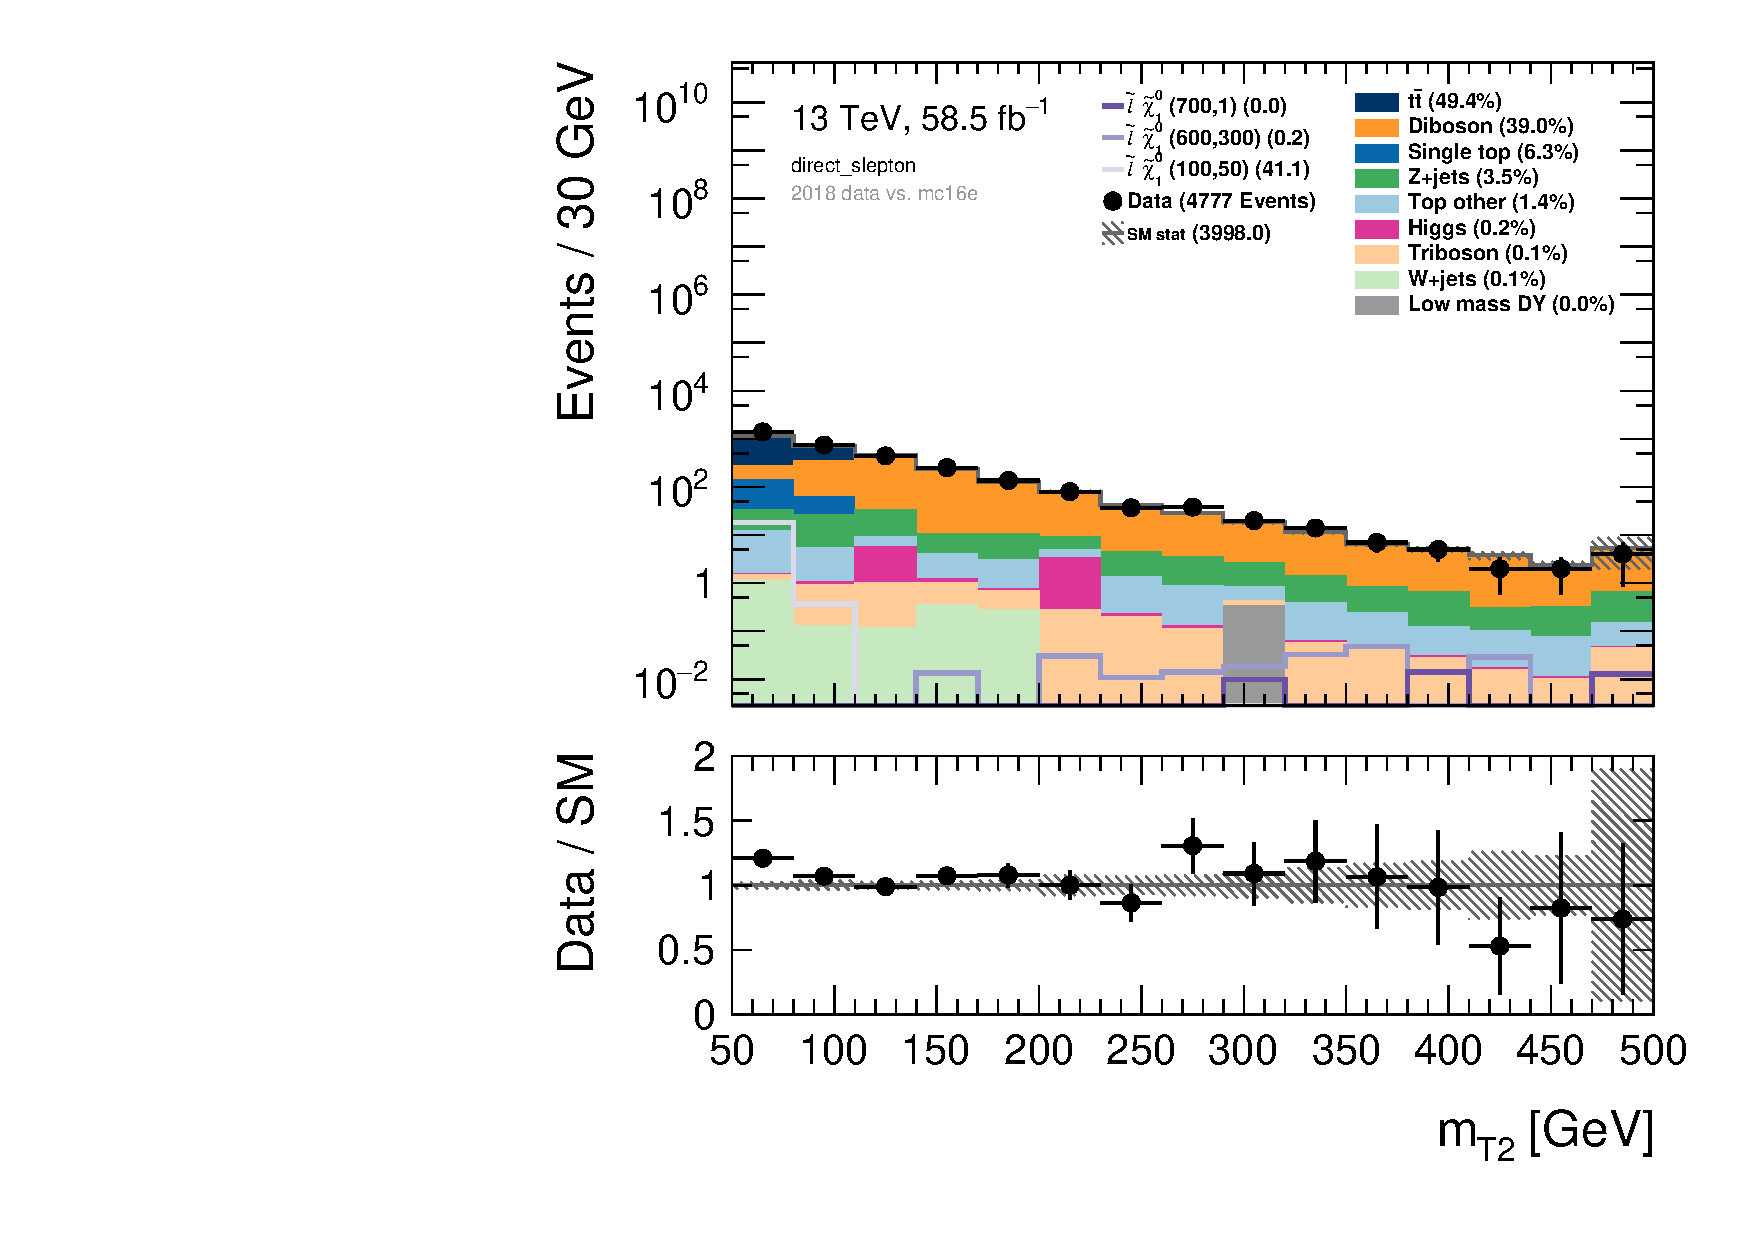
\includegraphics[width=\textwidth]{Figures/SlepSlep/CutAndCount/3rdcut_Zveto/hist1d_mt2_direct_slepton.pdf}
    \caption{Stransverse mass}
    \label{fig:my_label}
    \end{subfigure}
    \begin{subfigure}[t!]{0.49\textwidth}
        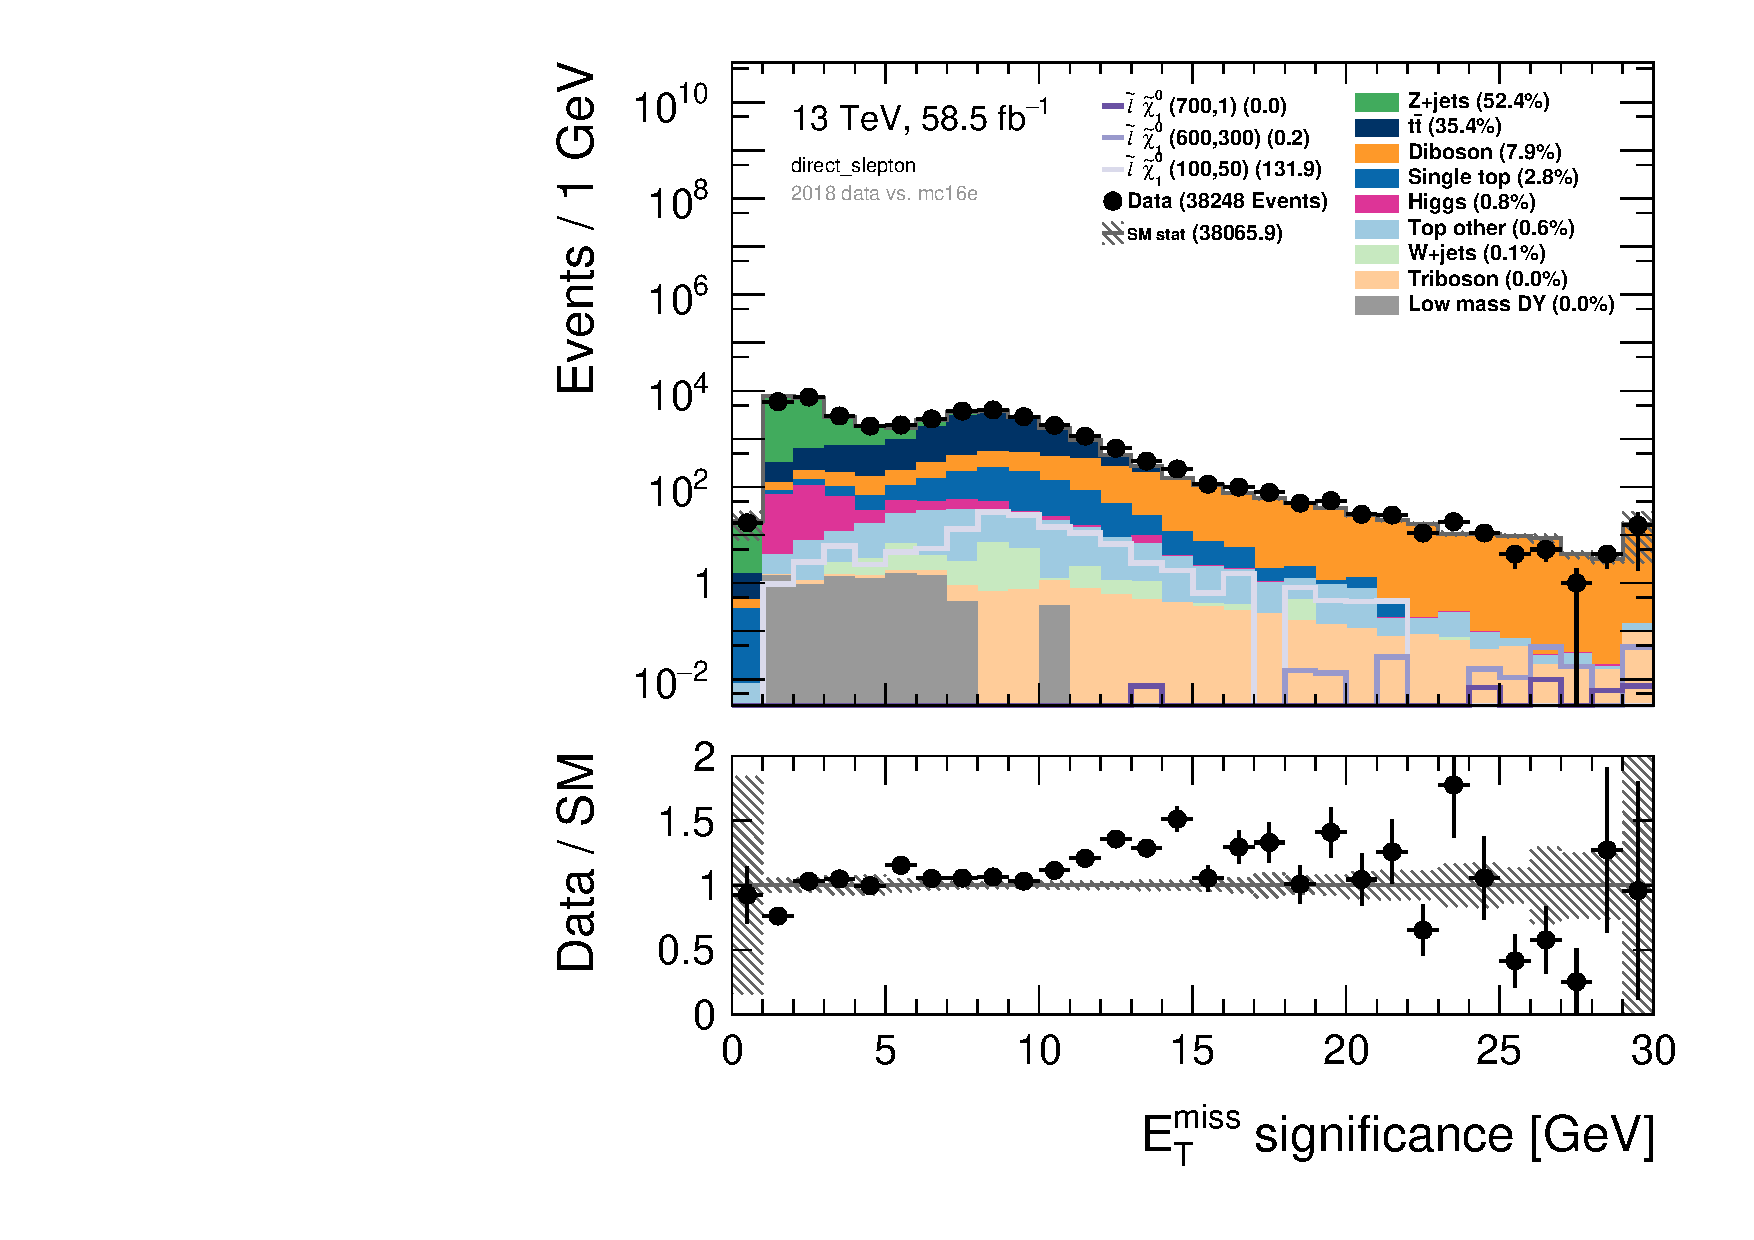
\includegraphics[width=\textwidth]{Figures/SlepSlep/CutAndCount/3rdcut_Zveto/hist1d_met_Sign_direct_slepton.pdf}
    \caption{Missing transverse energy significance}
    \label{fig:my_label}
    \end{subfigure}
    \caption{Plot of the four most important variables in direct slepton production with a cut on $E_T^{miss} >110$, $E_T^{miss}$ significance $>10$ and a Z-veto in addition to the previous cuts.}
    \label{fig:slepslep3rdcut}
\end{figure}



After adding some jet cuts (number of jets with $p_T$> 30GeV = 0 and a b-jet veto) we get the results in figure \ref{fig:slepslep4th_3_cut}. We can see that we succeeded on reducing the $t\Bar{t}$ background as well and we now have diboson as the dominating background.

\begin{figure}[H]
%\begin{minipage}{2\textwidth}
%\begin{adjustwidth}{-3cm}{-3cm}
\centering
%\advance\leftskip-4cm 
%\advance\rightskip-4cm 
    \begin{subfigure}[t!]{0.49\textwidth}
        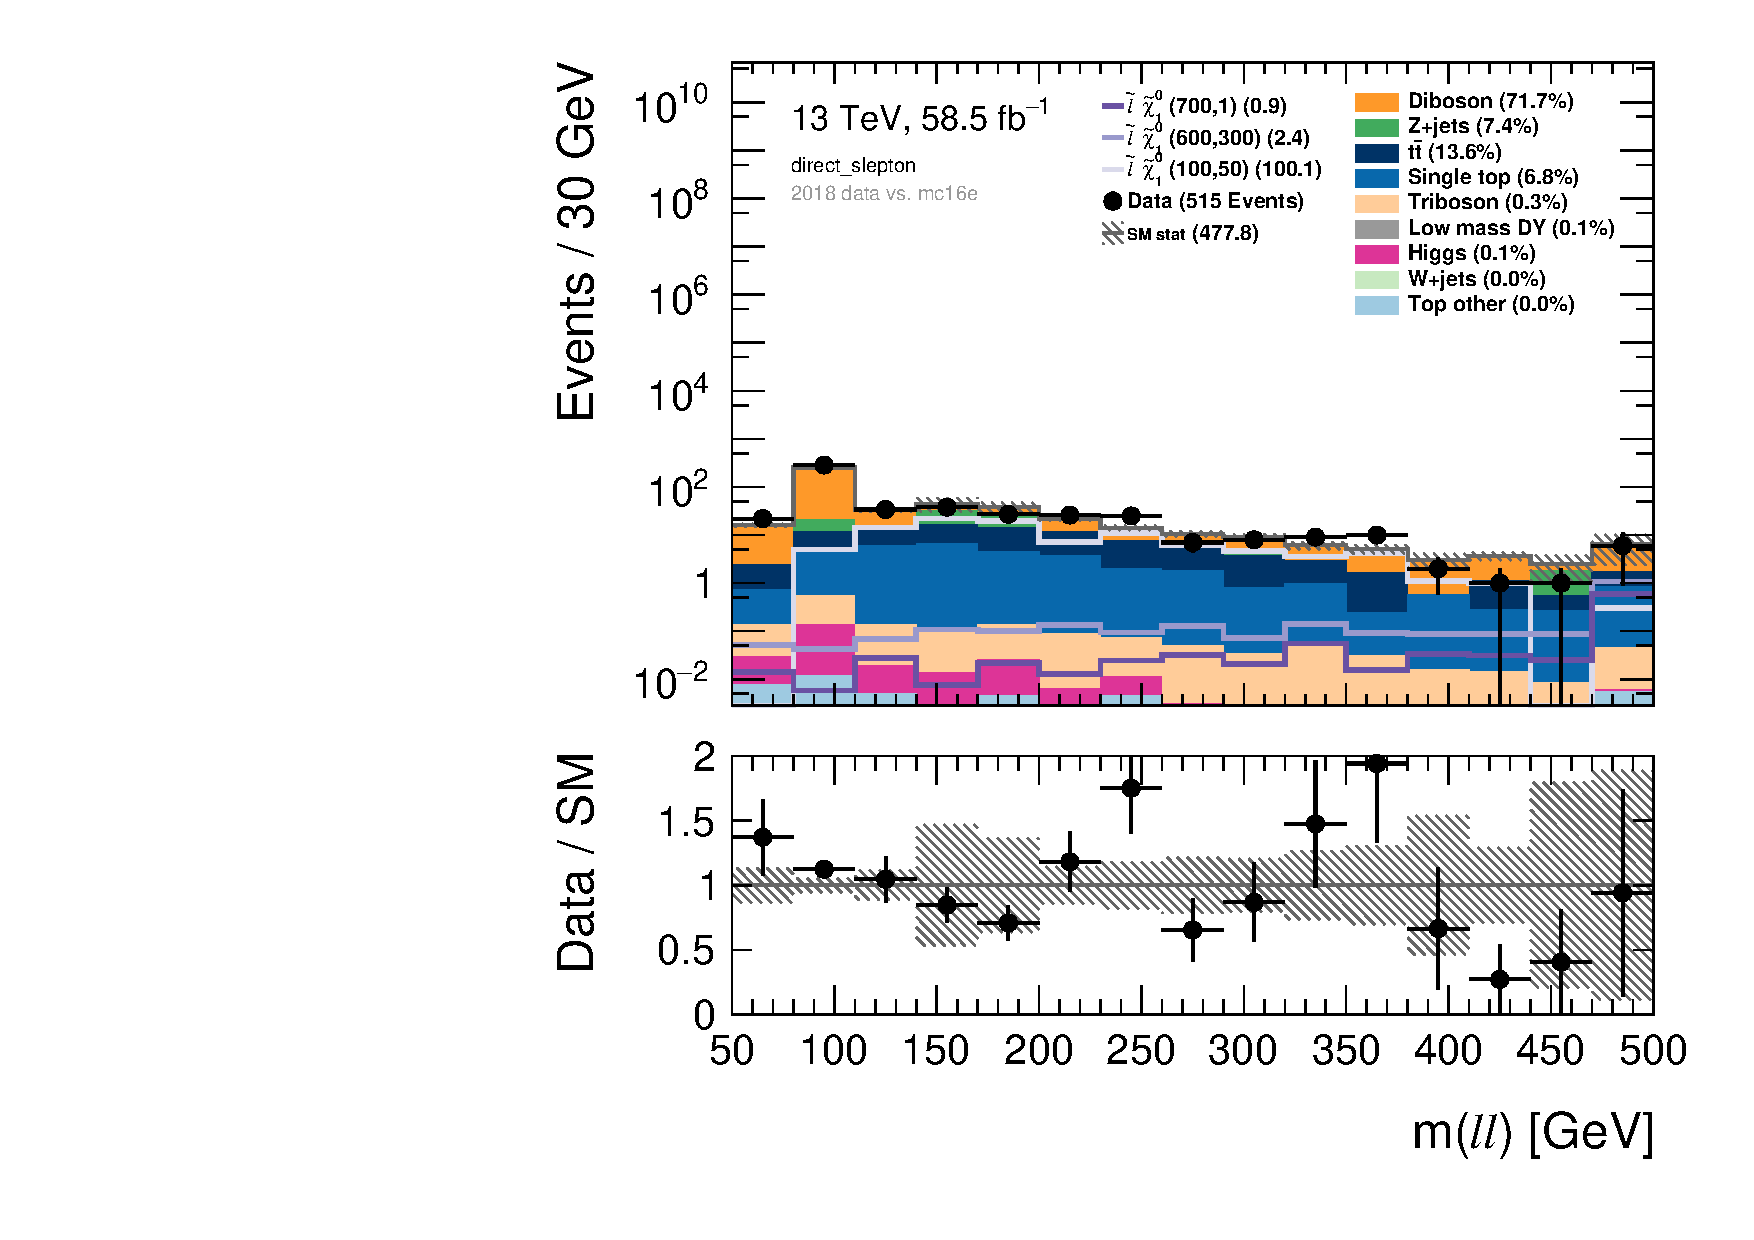
\includegraphics[width=\textwidth]{Figures/SlepSlep/CutAndCount/4thcut_3_Bjets/hist1d_mll_direct_slepton.pdf}
    \caption{Invariant mass}
    \label{fig:my_label}
    \end{subfigure}
    \begin{subfigure}[t!]{0.49\textwidth}
        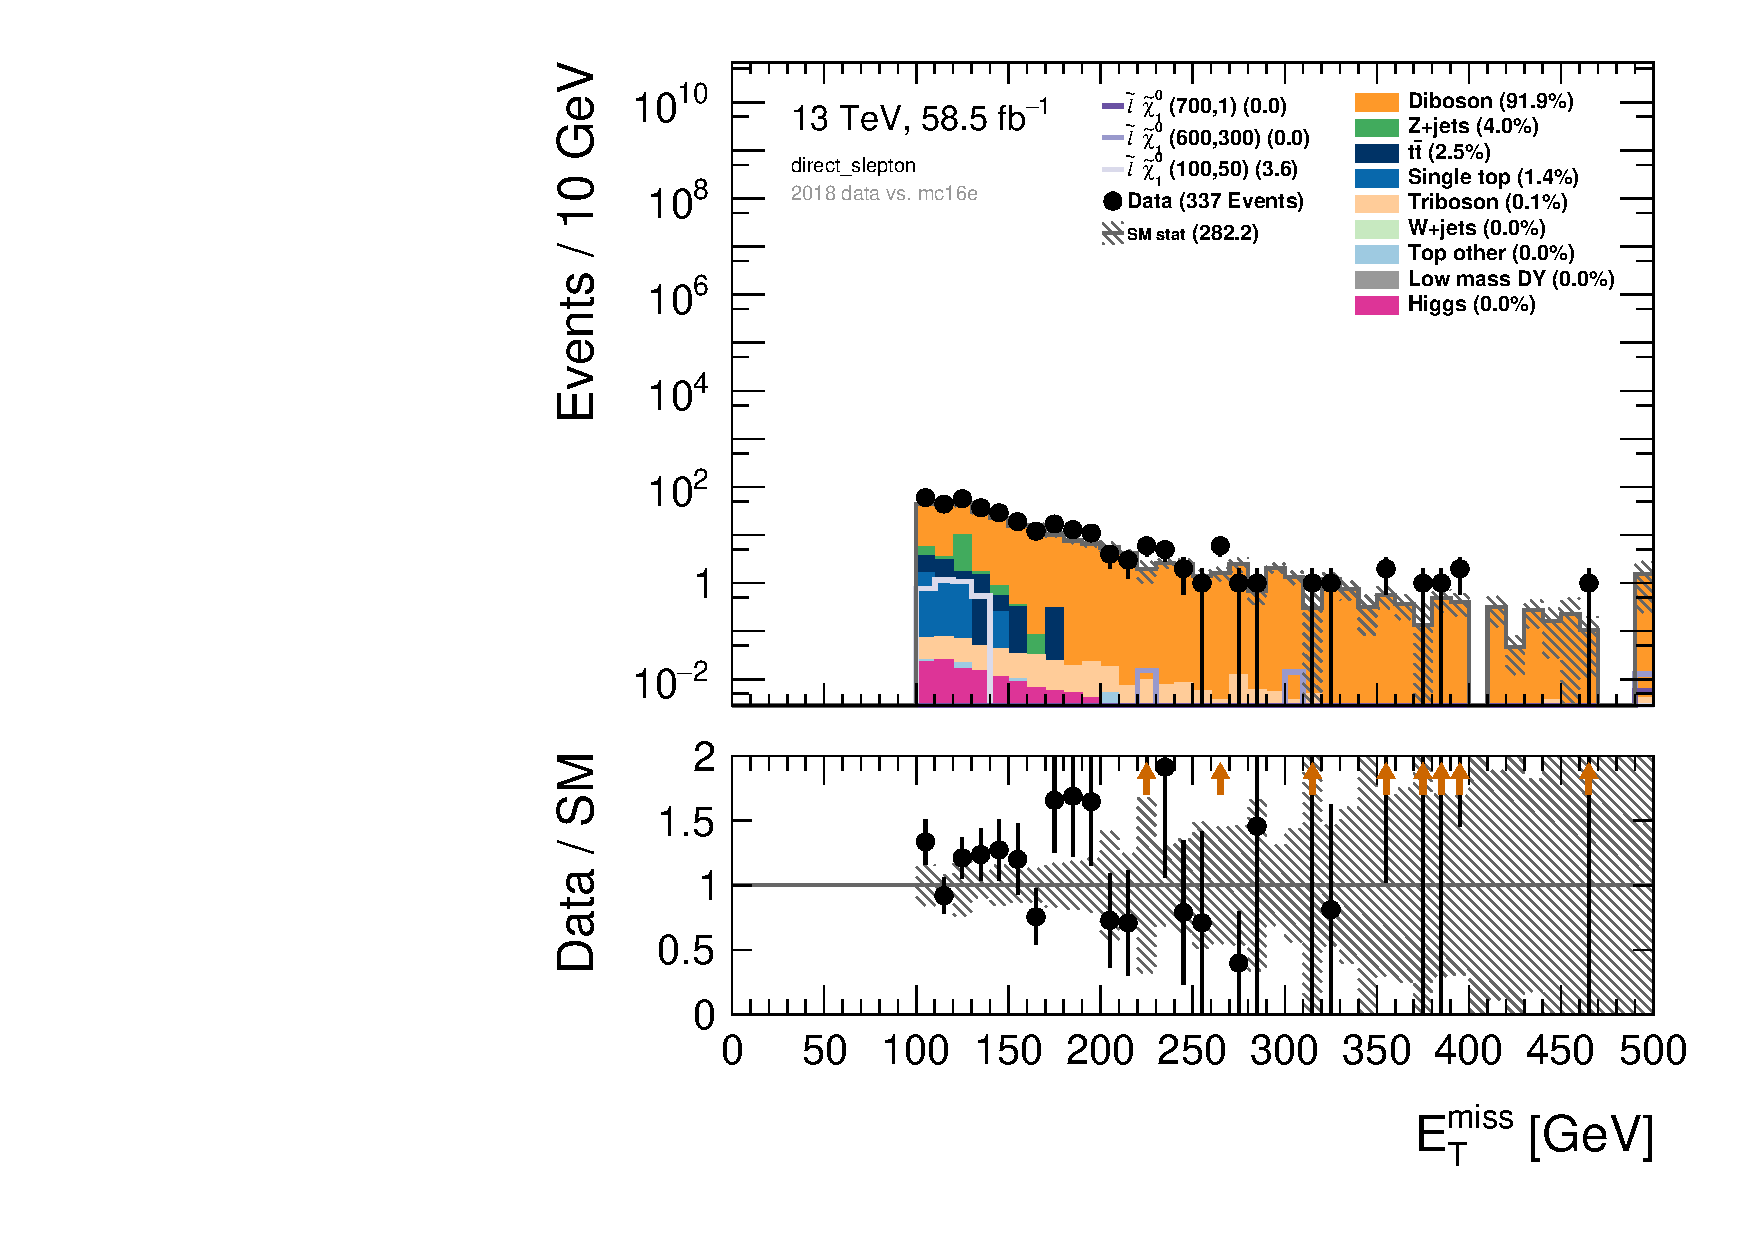
\includegraphics[width=\textwidth]{Figures/SlepSlep/CutAndCount/4thcut_3_Bjets/hist1d_met_Et_direct_slepton.pdf}
    \caption{Missing transverse energy}
    \label{fig:my_label}
    \end{subfigure}
    \\
    \begin{subfigure}[t!]{0.49\textwidth}
        \includegraphics[width=\textwidth]{Figures/SlepSlep/CutAndCount/4thcut_3_Bjets/hist1d_mt2_direct_slepton.pdf}
    \caption{Stransverse mass}
    \label{fig:my_label}
    \end{subfigure}
    \begin{subfigure}[t!]{0.49\textwidth}
        \includegraphics[width=\textwidth]{Figures/SlepSlep/CutAndCount/4thcut_3_Bjets/hist1d_met_Sign_direct_slepton.pdf}
    \caption{Missing transverse energy significance}
    \label{fig:my_label}
    \end{subfigure}
    \caption{Plot of the four most important variables in direct slepton production with a cut on number of jets and b-jets = 0 in addition to the previous cuts.}
    \label{fig:slepslep4th_3_cut}
\end{figure}

After adding one last cut in the $m_{T_2}$  variable we can see that the background doesn't change that much and that our signals is almost cut away as well. 

\begin{figure}[H]
%\begin{minipage}{2\textwidth}
%\begin{adjustwidth}{-3cm}{-3cm}
\centering
%\advance\leftskip-4cm 
%\advance\rightskip-4cm 
    \begin{subfigure}[t!]{0.49\textwidth}
        \includegraphics[width=\textwidth]{Figures/SlepSlep/CutAndCount/5thcut_1_mt2_100/hist1d_mll_direct_slepton.pdf}
    \caption{Invariant mass}
    \label{fig:my_label}
    \end{subfigure}
    \begin{subfigure}[t!]{0.49\textwidth}
        \includegraphics[width=\textwidth]{Figures/SlepSlep/CutAndCount/5thcut_1_mt2_100/hist1d_met_Et_direct_slepton.pdf}
    \caption{Missing transverse energy}
    \label{fig:my_label}
    \end{subfigure}
    \\
    \begin{subfigure}[t!]{0.49\textwidth}
        \includegraphics[width=\textwidth]{Figures/SlepSlep/CutAndCount/5thcut_1_mt2_100/hist1d_mt2_direct_slepton.pdf}
    \caption{Stransverse mass}
    \label{fig:my_label}
    \end{subfigure}
    \begin{subfigure}[t!]{0.49\textwidth}
        \includegraphics[width=\textwidth]{Figures/SlepSlep/CutAndCount/5thcut_1_mt2_100/hist1d_met_Sign_direct_slepton.pdf}
    \caption{Missing transverse energy significance}
    \label{fig:my_label}
    \end{subfigure}
    \caption{Plot of the four most important variables in direct slepton production with a cut on $m_{T_2} > 100$ GeV in addition to the previous cuts.}
    \label{fig:slepslep5th_1_cut}
\end{figure}


After adding all of the cuts mentioned above we can see that the signal almost no longer is present which is pretty bad when we want to see if the data follows the signal or the background. Since this isn't working that well, we are going to try to see if cuts found by ML is a better solution. 

\end{comment}















\begin{comment}


\begin{figure}[H]
%\begin{minipage}{2\textwidth}
%\begin{adjustwidth}{-3cm}{-3cm}
\centering
%\advance\leftskip-4cm 
%\advance\rightskip-4cm 
    \begin{subfigure}[t!]{0.49\textwidth}
        \includegraphics[width=\textwidth]{Figures/SlepSlep/CutAndCount/1stcut_2L+OS/hist1d_mll_direct_slepton.pdf}
%    \caption{Caption}
    \label{fig:my_label}
    \end{subfigure}
    \begin{subfigure}[t!]{0.49\textwidth}
        \includegraphics[width=\textwidth]{Figures/SlepSlep/CutAndCount/1stcut_2L+OS/hist1d_met_Et_direct_slepton.pdf}
 %   \caption{Caption}
    \label{fig:my_label}
    \end{subfigure}
    \\
    \begin{subfigure}[t!]{0.49\textwidth}
        \includegraphics[width=\textwidth]{Figures/SlepSlep/CutAndCount/1stcut_2L+OS/hist1d_mt2_direct_slepton.pdf}
  %  \caption{Caption}
    \label{fig:my_label}
    \end{subfigure}
    \begin{subfigure}[t!]{0.49\textwidth}
        \includegraphics[width=\textwidth]{Figures/SlepSlep/CutAndCount/1stcut_2L+OS/hist1d_nBJet20_MV2c10_FixedCutBEff_77_direct_slepton.pdf}
  %  \caption{Caption}
    \label{fig:my_label}
    \end{subfigure}
    \\
    \begin{subfigure}[t!]{0.49\textwidth}
        \includegraphics[width=\textwidth]{Figures/SlepSlep/CutAndCount/1stcut_2L+OS/hist1d_nJet20_direct_slepton.pdf}
%    \caption{Caption}
    \label{fig:my_label}
    \end{subfigure}
    \begin{subfigure}[t!]{0.49\textwidth}
        \includegraphics[width=\textwidth]{Figures/SlepSlep/CutAndCount/1stcut_2L+OS/hist1d_nJet30_direct_slepton.pdf}
 %   \caption{Caption}
    \label{fig:my_label}
    \end{subfigure}
\end{figure}

\begin{figure}[H]
%\begin{minipage}{2\textwidth}
%\begin{adjustwidth}{-3cm}{-3cm}
\centering
%\advance\leftskip-4cm 
%\advance\rightskip-4cm 
    \begin{subfigure}[t!]{0.49\textwidth}
        \includegraphics[width=\textwidth]{Figures/SlepSlep/CutAndCount/1stcut_2L+OS/hist1d_lepPt[0]_direct_slepton.pdf}
%    \caption{Caption}
    \label{fig:my_label}
    \end{subfigure}
    \begin{subfigure}[t!]{0.49\textwidth}
        \includegraphics[width=\textwidth]{Figures/SlepSlep/CutAndCount/1stcut_2L+OS/hist1d_lepPt[1]_direct_slepton.pdf}
 %   \caption{Caption}
    \\
    \label{fig:my_label}
    \end{subfigure}
    \begin{subfigure}[t!]{0.49\textwidth}
        \includegraphics[width=\textwidth]{Figures/SlepSlep/CutAndCount/1stcut_2L+OS/hist1d_lepPt_direct_slepton.pdf}
  %  \caption{Caption}
    \label{fig:my_label}
    \end{subfigure}
    \begin{subfigure}[t!]{0.49\textwidth}
        \includegraphics[width=\textwidth]{Figures/SlepSlep/CutAndCount/1stcut_2L+OS/hist1d_pTdiff_direct_slepton.pdf}
%    \caption{Caption}
    \\
    \label{fig:my_label}
    \end{subfigure}
    \begin{subfigure}[t!]{0.49\textwidth}
        \includegraphics[width=\textwidth]{Figures/SlepSlep/CutAndCount/1stcut_2L+OS/hist1d_deltaRll_direct_slepton.pdf}
 %   \caption{Caption}
    \label{fig:my_label}
    \end{subfigure}
    \begin{subfigure}[t!]{0.49\textwidth}
        \includegraphics[width=\textwidth]{Figures/SlepSlep/CutAndCount/1stcut_2L+OS/hist1d_deltaPhi_direct_slepton.pdf}
  %  \caption{Caption}
    \label{fig:my_label}
    \end{subfigure}
\end{figure}

\begin{figure}[H]
%\begin{minipage}{2\textwidth}
%\begin{adjustwidth}{-3cm}{-3cm}
\centering
    \begin{subfigure}[t!]{0.49\textwidth}
        \includegraphics[width=\textwidth]{Figures/SlepSlep/CutAndCount/1stcut_2L+OS/hist1d_met_HT_direct_slepton.pdf}
%    \caption{Caption}
    \label{fig:my_label}
    \end{subfigure}
    \begin{subfigure}[t!]{0.49\textwidth}
        \includegraphics[width=\textwidth]{Figures/SlepSlep/CutAndCount/1stcut_2L+OS/hist1d_HT_direct_slepton.pdf}
 %   \caption{Caption}
    \label{fig:my_label}
    \end{subfigure}
%\end{adjustwidth}
\end{figure}
\end{comment}





